% Preamble
\documentclass[a4paper,12pt]{article}

% Prevents line breaks mid-word
\tolerance=1
\emergencystretch=\maxdimen
\hyphenpenalty=10000
\hbadness=10000

% Packages
\usepackage{amsfonts}
\usepackage{blindtext}
\usepackage{titlesec}
\usepackage{todonotes}
\usepackage{setspace}
\usepackage[hidelinks]{hyperref}

\usepackage{graphicx}
\graphicspath{{images/}}

\usepackage{biblatex}
\addbibresource{bibliography.bib}

 % Set inline as default for todos
\usepackage{regexpatch}
\makeatletter
\xpatchcmd{\@todo}{\setkeys{todonotes}{#1}}{\setkeys{todonotes}{inline,#1}}{}{}
\makeatother

% Document
\begin{document}
    \begin{titlepage}
        \centering
        
\includegraphics[width = 1\textwidth]{UoB_Logo}\\[10ex]
        \Huge{A Comparison of Approaches to Combinatorial Optimisation for Multi-Day Route Planning}\\[14ex]
        \LARGE{Jacob Luck}\\
        \large{2338114}\\[2ex]
        \Large{B.Sc. Computer Science with a Year in Industry}\\
        \Large{Project Supervisor - Leandro Minku}\\[2ex]
        \large{April 2025}\\
        \large{xxxx Words}
    \end{titlepage}

    \doublespacing

    \section*{Abstract}\label{sec:abstract}
    \todo{Write abstract}

    \pagebreak

    \tableofcontents

    \pagebreak

    \section{Introduction}\label{sec:introduction}
    \subsection{Motivation}\label{subsec:motivation}
    \todo{Write about reasoning for this project, can copy a little bit over from presentation slides. Explain problem informally. Link into aims and objectives.}
    \subsection{Aims and Objectives}\label{subsec:aims-and-objectives}
    \todo{Explin goals of the project, link in to methodology.}
    \subsection{Methodology}\label{subsec:methodology}
    \todo{Briefly explain how the project will be carried out. A more thorough description can be provided later on, i.e., when describing algorithms.}
    \subsection{Summary}\label{subsec:summary}
    \todo{Explain what is in the rest of the report. "In this report I shall...", cover each section, etc.}

    \pagebreak

    \section{Problem Formulation}\label{sec:problem-formulation}
    \subsection{Problem Description}\label{subsec:problem-description}
Given a positive integer $d$ and a graph $G = (V, E)$, where $V$ is set of locations including a designated
starting point $s$ and $E$ is a set of weighted edges linking every location to every other location, find a route
that:
\begin{enumerate}
    \item Visits all nodes $V \setminus c$ once.
    \item Starts and finishes at $s$, having visited it $d$ times, without ever visiting consecutively.
    \item Minimises both the cumulative edge weights in the route and the variance in cumulative weight between
    each visit to $s$.
\end{enumerate}

\subsection{Inputs, Outputs and Design Variables}\label{subsec:inputs-and-outputs}
Inputs:
\begin{itemize}
    \item $d$: The number of times $s$ should be visited in a route.
    Contextually, $d$ represents the number of days a tourist will spend on their trip. $d \in \mathbb{Z}, d > 0$
    \item $G = (V, E)$: A pair comprising:
    \begin{itemize}
        \item[\textbullet] $V$: A set of nodes representing locations the tourist would like to visit.
        $v \in V, v = (x, y, t)$, a triple comprising:
        \begin{itemize}
            \item[\textbullet]$x$: Longitude, indicating the location's geographic east-west position on the
            earth\footnote{\label{latitude-longitude-note}While the coordinates of our locations are
            included in $V$, they are not directly tied to the weight of our edges $E$, which are based on
            time and not distance.}.\\
            $x \in \mathbb{Q}, -180 \leq x \leq 180$.
            \item[\textbullet]$y$: Latitude, indicating the location's geographic north-south position on
            the earth\footnote{See footnote \ref{latitude-longitude-note}}.\\
            $y \in \mathbb{Q}, -90 \leq y \leq 90$.
            \item[\textbullet]$t$: Duration, in minutes, indicating how much time to spend at this location.\\
            $t \in \mathbb{Z}, t > 0$.
        \end{itemize}
        \item[\textbullet] $E$: A set of edges $e \in E$ that connects every node to every other node,
        bidirectionally. $e = (v_1, v_2, w)$, a triple comprising of:
        \begin{itemize}
            \item[\textbullet]$v_1$: A location representing the origin of the edge.\\
            $v_1 \in V$.
            \item[\textbullet]$v_2$: A location representing the destination of the edge.\\
            $v_2 \in V$.
            \item[\textbullet]$w$: A weight indicating the sum of the time it takes to travel from $v_1$ to $v_2$
            and the time the tourist wishes to spent at $v_2$.\\
            $w \in Z, w > 0$.
        \end{itemize}
    \end{itemize}
    \item $s$: Starting point that should be visited $d$ times.
    Contextually, $s$ represents where the tourist is staying and will return to at the end of each day.\\
    $s \in V$.
\end{itemize}
Outputs:
    \begin{itemize}
    \item $R$: A valid route satisfying all constraints, represented as an ordered sequence of locations.\\
    $R = [r_1, r_2, \dots, r_n], r_i \in V$.
\end{itemize}

\subsection{Objective Function}\label{subsec:objective-function}
As previously mentioned in the \hyperref[subsec:problem-description]{Problem Description}, our goal is to find a
route that minimises the cumulative weight and the variance in route weight between each visit to $s$.
To accomplish this the following cost function is applied to each route:
\todo{Update equation for cost, talk to leandro about how to handle changing this.}
\begin{equation}
    Cost(R) = W \times (1 + \sigma)\label{eq:cost}
\end{equation}
Where $W$ is the sum of the weights of all edges traversed in the route and $\sigma$ is the standard deviation of the
sum of weights between each visit to $s$:
\begin{equation}
    W = \sum_{i=0}^{n-1} w(r_i, r_{i+1}), r_i \in R\label{eq:weight}
\end{equation}
Where $w(r_i, r_{i+1})$ is the weight of the edge between $r_i$ and $r_{i+1}$.
\begin{equation}
    \sigma = \sqrt{\frac{\sum_{i=0}^{d}(x_i-\mu)}{d}}, x_i \in X\label{eq:standard-deviation}
\end{equation}
Where $R$ is divided into sections between each visit to $s$ and $X$ is a list of the sum of weights within these
sections.\\
$\mu$ is the mean cumulative weight of each $x_i$.

\subsection{Constraints}\label{subsec:constraints}
\todo{Describe constraints}

    \pagebreak

    \section{Literature Review}\label{sec:literature-review}
    \todo{Plan (and write) literature review}
    \todo{Remember to write about the strengths and weaknesses of existing work. At the end of this chapter you can then give a summary of the gaps that you'll be trying to improve with your work, and on the strengths that you will be maintaining in your work.}
    This literature review aims to explore existing research and approaches to other combinatorial optimization problems.
There is extensive previous research on various combinatorial problems, for example, the Travelling Salesman
Problem (TSP), Vehicle Routing Problem (VRP) and Tourist Trip Design Problem (TTDP).
It is important to understand how these problems are similar to the one presented in this report, as well as where
those similarities end.
By gaining an understanding of the strengths and limitations of existing approaches to similar problem, we can make
better informed decisions regarding which approaches to investigate, how they may be adapted to suit our specific
constraints and how they might be implemented in practice.
While the approaches taken to these problems may not be directly applicable to our own, it is likely we can adapt their
techniques to suit the specific constraints of this problem.

[paper1] defines [problem1] as [definition].
blah blah blah.
This is similar to our problem because [reason].
Another problem is [problem1], which is defined by [paper2] as [definition].
blah blah blah.
This is similar to our problem because [reason].

[paper3] proposes a solution to [problem] using [approach].
blah blah blah, pros, cons, etc.

READ, YOU NEED TO READ THE PAPERS stop faffing about and read the papers


\subsection{Related Optimization Problems}
\begin{itemize}
    \item Vehicle Routing Problems (VRP), particularly Multiple-Trip VRP (Cattaruzza et al., 2016)
    \item Traveling Salesman Problem variants (Applegate et al., 2006)
    \item Tourist Trip Design Problem (TTDP) (Vansteenwegen et al., 2011; Gavalas et al., 2014)
    \item Orienteering Problems with time constraints (Gunawan et al., 2016)
\end{itemize}

\subsection{Algorithms for Multi-Visit Routing}
\begin{itemize}
    \item Exact methods: Branch and Bound, Dynamic Programming, Integer Linear Programming (Laporte, 1992)
    \item Heuristic approaches for multi-visit scenarios (Necula et al., 2015)
    \item Metaheuristics: Genetic Algorithms (Potvin, 1996), Simulated Annealing (Černý, 1985), Ant Colony Optimization (Dorigo \& Gambardella, 1997)
    \item Approaches handling returning to a depot multiple times (Azi et al., 2014)
\end{itemize}

\subsection{Multi-Objective Optimization Approaches}
\begin{itemize}
    \item Survey of approaches for handling multiple objectives
    \begin{itemize}
        \item Weighted sum methods (Marler \& Arora, 2010)
        \item Pareto optimization approaches (García-Nájera et al., 2013)
        \item Constraint-based methods (Konak et al., 2006)
    \end{itemize}
    \item Techniques for minimizing variance/balancing workloads (Dutot et al., 2006; Ghannadpour et al., 2013)
\end{itemize}

\subsection{Time-Constrained Route Optimization}
\begin{itemize}
    \item Handling time windows and duration constraints (Toth \& Vigo, 2002)
    \item Techniques for time-dependent weights (Gendreau et al., 2015)
    \item Applications to tourist trip planning with time budgets (Souffriau et al., 2013)
\end{itemize}

\subsection{Real-World Applications}
\begin{itemize}
    \item Implementation considerations for tourist route planning systems (Souffriau et al., 2008)
    \item Personalized itinerary systems and their algorithms (Schaller et al., 2014)
    \item Case studies of similar optimization problems in practice (Gavalas et al., 2015)
\end{itemize}

\subsection{Gap Analysis and Research Directions}
\begin{itemize}
    \item Identify how existing approaches fall short for this specific combination of constraints
    \item How methods might be adapted or combined to address the problem (Liao et al., 2017)
    \item Novel aspects requiring new algorithmic development (Nazari et al., 2018; Chou et al., 2020)
\end{itemize}

\subsection{Conclusion}
\begin{itemize}
    \item Summarize the key algorithmic approaches most relevant to this problem
    \item Identify the most promising directions based on the literature
    \item Transition to the approach taken in the current research
\end{itemize}

Full references (you'll need to format these according to your preferred citation style):

Applegate, D. L., Bixby, R. E., Chvátal, V., & Cook, W. J. (2006). The traveling salesman problem: a computational study. Princeton University Press.
Azi, N., Gendreau, M., & Potvin, J. Y. (2014). An exact algorithm for a vehicle routing problem with time windows and multiple use of vehicles. European Journal of Operational Research, 202(3), 756-763.
Cattaruzza, D., Absi, N., Feillet, D., & Vidal, T. (2016). The multi-trip vehicle routing problem with time windows and release dates. Transportation Research Part E: Logistics and Transportation Review, 92, 118-133.
Černý, V. (1985). Thermodynamical approach to the traveling salesman problem: An efficient simulation algorithm. Journal of Optimization Theory and Applications, 45(1), 41-51.
Chou, C. C., Fu, J. S., Kuo, S. P., & Li, P. H. (2020). A hybrid algorithm of simulated annealing and tabu search for the bi-objective team orienteering problem with time windows. IEEE Access, 8, 72564-72578.
Dorigo, M., & Gambardella, L. M. (1997). Ant colony system: a cooperative learning approach to the traveling salesman problem. IEEE Transactions on evolutionary computation, 1(1), 53-66.
Dutot, P. F., Laugier, A., & Bustos, A. M. (2006). Balancing a dynamic mobile workforce via constraint-based local search. In International Conference on Innovative Techniques and Applications of Artificial Intelligence (pp. 35-48).
García-Nájera, A., Bullinaria, J. A., & Gutiérrez-Andrade, M. A. (2013). A Pareto ant colony optimization algorithm for the multi-objective tourist trip design problem. In Applications of Evolutionary Computation (pp. 143-154).
Gavalas, D., Konstantopoulos, C., Mastakas, K., & Pantziou, G. (2014). Models and algorithms for the tourist trip design problem. Annals of Operations Research, 224(1), 65-86.
Gavalas, D., Konstantopoulos, C., Mastakas, K., & Pantziou, G. (2015). A variable neighborhood search approach for the tourist trip design problem. Expert Systems with Applications, 42(21), 7911-7919.
Gendreau, M., Ghiani, G., & Guerriero, E. (2015). Time-dependent routing problems: A review. Computers & Operations Research, 64, 189-197.
Ghannadpour, S. F., Noori, S., Tavakkoli-Moghaddam, R., & Ghoseiri, K. (2013). A multi-objective vehicle routing problem with soft time windows: The minimization of drivers' dissatisfaction. Transportation Research Part E: Logistics and Transportation Review, 53, 64-77.
Gunawan, A., Lau, H. C., & Vansteenwegen, P. (2016). Orienteering problem: A survey of recent variants, solution approaches and applications. European Journal of Operational Research, 255(2), 315-332.
Konak, A., Coit, D. W., & Smith, A. E. (2006). Multi-objective optimization using genetic algorithms: A tutorial. Reliability Engineering & System Safety, 91(9), 992-1007.
Laporte, G. (1992). The traveling salesman problem: An overview of exact and approximate algorithms. European Journal of Operational Research, 59(2), 231-247.
Liao, T. W., Egbelu, P. J., & Chang, P. C. (2017). Integrated manufacturing systems design with robot movement simulation and multi-objective genetic algorithms. International Journal of Production Research, 55(15), 4399-4422.
Marler, R. T., & Arora, J. S. (2010). The weighted sum method for multi-objective optimization: new insights. Structural and Multidisciplinary Optimization, 41(6), 853-862.
Nazari, M., Oroojlooy, A., Snyder, L., & Takác, M. (2018). Reinforcement learning for solving the vehicle routing problem. Advances in Neural Information Processing Systems, 31.
Necula, R., Breaban, M., & Raschip, M. (2015). Exact and heuristic approaches for the multi-visit salesman problem. In International Conference on Computational Collective Intelligence (pp. 357-368).
Potvin, J. Y. (1996). Genetic algorithms for the traveling salesman problem. Annals of Operations Research, 63(3), 337-370.
Schaller, R., Elsweiler, D., & Harvey, M. (2014). City trip planner: Personalized itinerary planning for groups of people. In Proceedings of the 22nd International Conference on User Modeling, Adaptation, and Personalization (pp. 184-191).
Souffriau, W., Vansteenwegen, P., Vertommen, J., Berghe, G. V., & Oudheusden, D. V. (2008). A personalized tourist trip design algorithm for mobile tourist guides. Applied Artificial Intelligence, 22(10), 964-985.
Souffriau, W., Vansteenwegen, P., & Oudheusden, D. V. (2013). The multi-constraint team orienteering problem with multiple time windows. Transportation Science, 47(1), 53-63.
Toth, P., & Vigo, D. (2002). The vehicle routing problem. SIAM.
Vansteenwegen, P., Souffriau, W., & Van Oudheusden, D. (2011). The orienteering problem: A survey. European Journal of Operational Research, 209(1), 1-10.

    \pagebreak

    \section{Algorithms Investigated}\label{sec:algorithms-investigated}
    Based on what was learned during the literature review, the decision was made to investigate three distinct approaches
to the Multi Day Route Planning problem:
\begin{itemize}
    \item Cluster then Route, where a clustering algorithm is used to group together locations in the input,
    before a routing algorithm is applied to each group.
    \item Route then Insert, where a route is found that visits all locations, before the end of each day is
    inserted somewhere appropriate in the route.
    \item Trip Generation, which aims to find a whole multi day trip in one step.
\end{itemize}
To form these approaches a number of clustering, routing and trip generation algorithms were implemented, with each
of these listed below:\\
\noindent
\textbf{Clustering}
\begin{itemize}
    \item K-Means Clustering,
    \item Genetic Clustering,
    \item Centroid-Based Genetic Clustering.
\end{itemize}\\
\noindent
\textbf{Routing}
\begin{itemize}
    \item Brute Force Routing,
    \item Greedy Routing,
    \item Greedy Insertion Routing\footnote{Greedy Insertion Routing will also be extended to allow its usage for splitting routes into multiple days.},
    \item Convex Hull Routing,
    \item Genetic Routing.
\end{itemize}\\
\noindent
\textbf{Trip Generation}
\begin{itemize}
    \item Brute Force Trip Generation,
    \item Genetic Trip Generation,
    \item Greedy Insertion Trip Generation.
\end{itemize}

\noindent
After describing the pre-requisites to implementing these algorithms, this section of the report will include a
description for all the algorithms listed above, as well as explain how each was implemented within python.

\subsection{Implementation Pre-Requisites}\label{subsec:implementation-pre-requisites}
There are two things needed before beginning to implement the chosen algorithms, a method for generating inputs on which
to use these algorithms, and an implementation of an objective function to enable the evaluation of routes.

\subsubsection{Input Generation}\label{subsubsec:input-generation}
For generating inputs Openrouteservice's Points of Interest (PoI) and Distance Matrix API services will be used.
With the PoI service, locations such as a city centres can be input, and a specified number of locations of interest
around the area will be returned.
The PoI service also allows the limitation of locations returned to certain categories and the identification of
specific that a user would likely be interested in visiting, for example points labelled `tourism', `historic' or
`arts and culture'.

After these locations have been identified, the Distance Matrix can be used to create a graph linking each location to
one another with a weight associated with travelling between them.
The API call to this service can be configured such that, instead of distance, the weights in the matrix represent
the time taken to travel between locations via public transport.
Unfortunately, the Distance Matrix service limits the number of locations in a call to 25, severely limiting the
size of input that can be test.
Other alternative API's were considered, such as the Google Maps API or Mapbox, but all the alternatives were either too
expensive or equally, if not more, restrictive.

With these, a list of durations associated with the found locations can be generated, as well as a number of days for
the trip, to finally have the input ready.

\subsubsection{Objective Function}\label{subsubsec:algorithms-objective-function}
As described in the \hyperref[sec:problem-formulation]{Problem Formulation}, the Multi-Day Planning Problem's objective
function aims to calculate a cost for a given trip.
This function is needed such that different approaches and algorithms can be compared based on the quality of their
results.
Figure~\ref{fig:Algorithm.evaluate_route} shows how this was implemented in this project.
\begin{figure}[H]
    \centering
    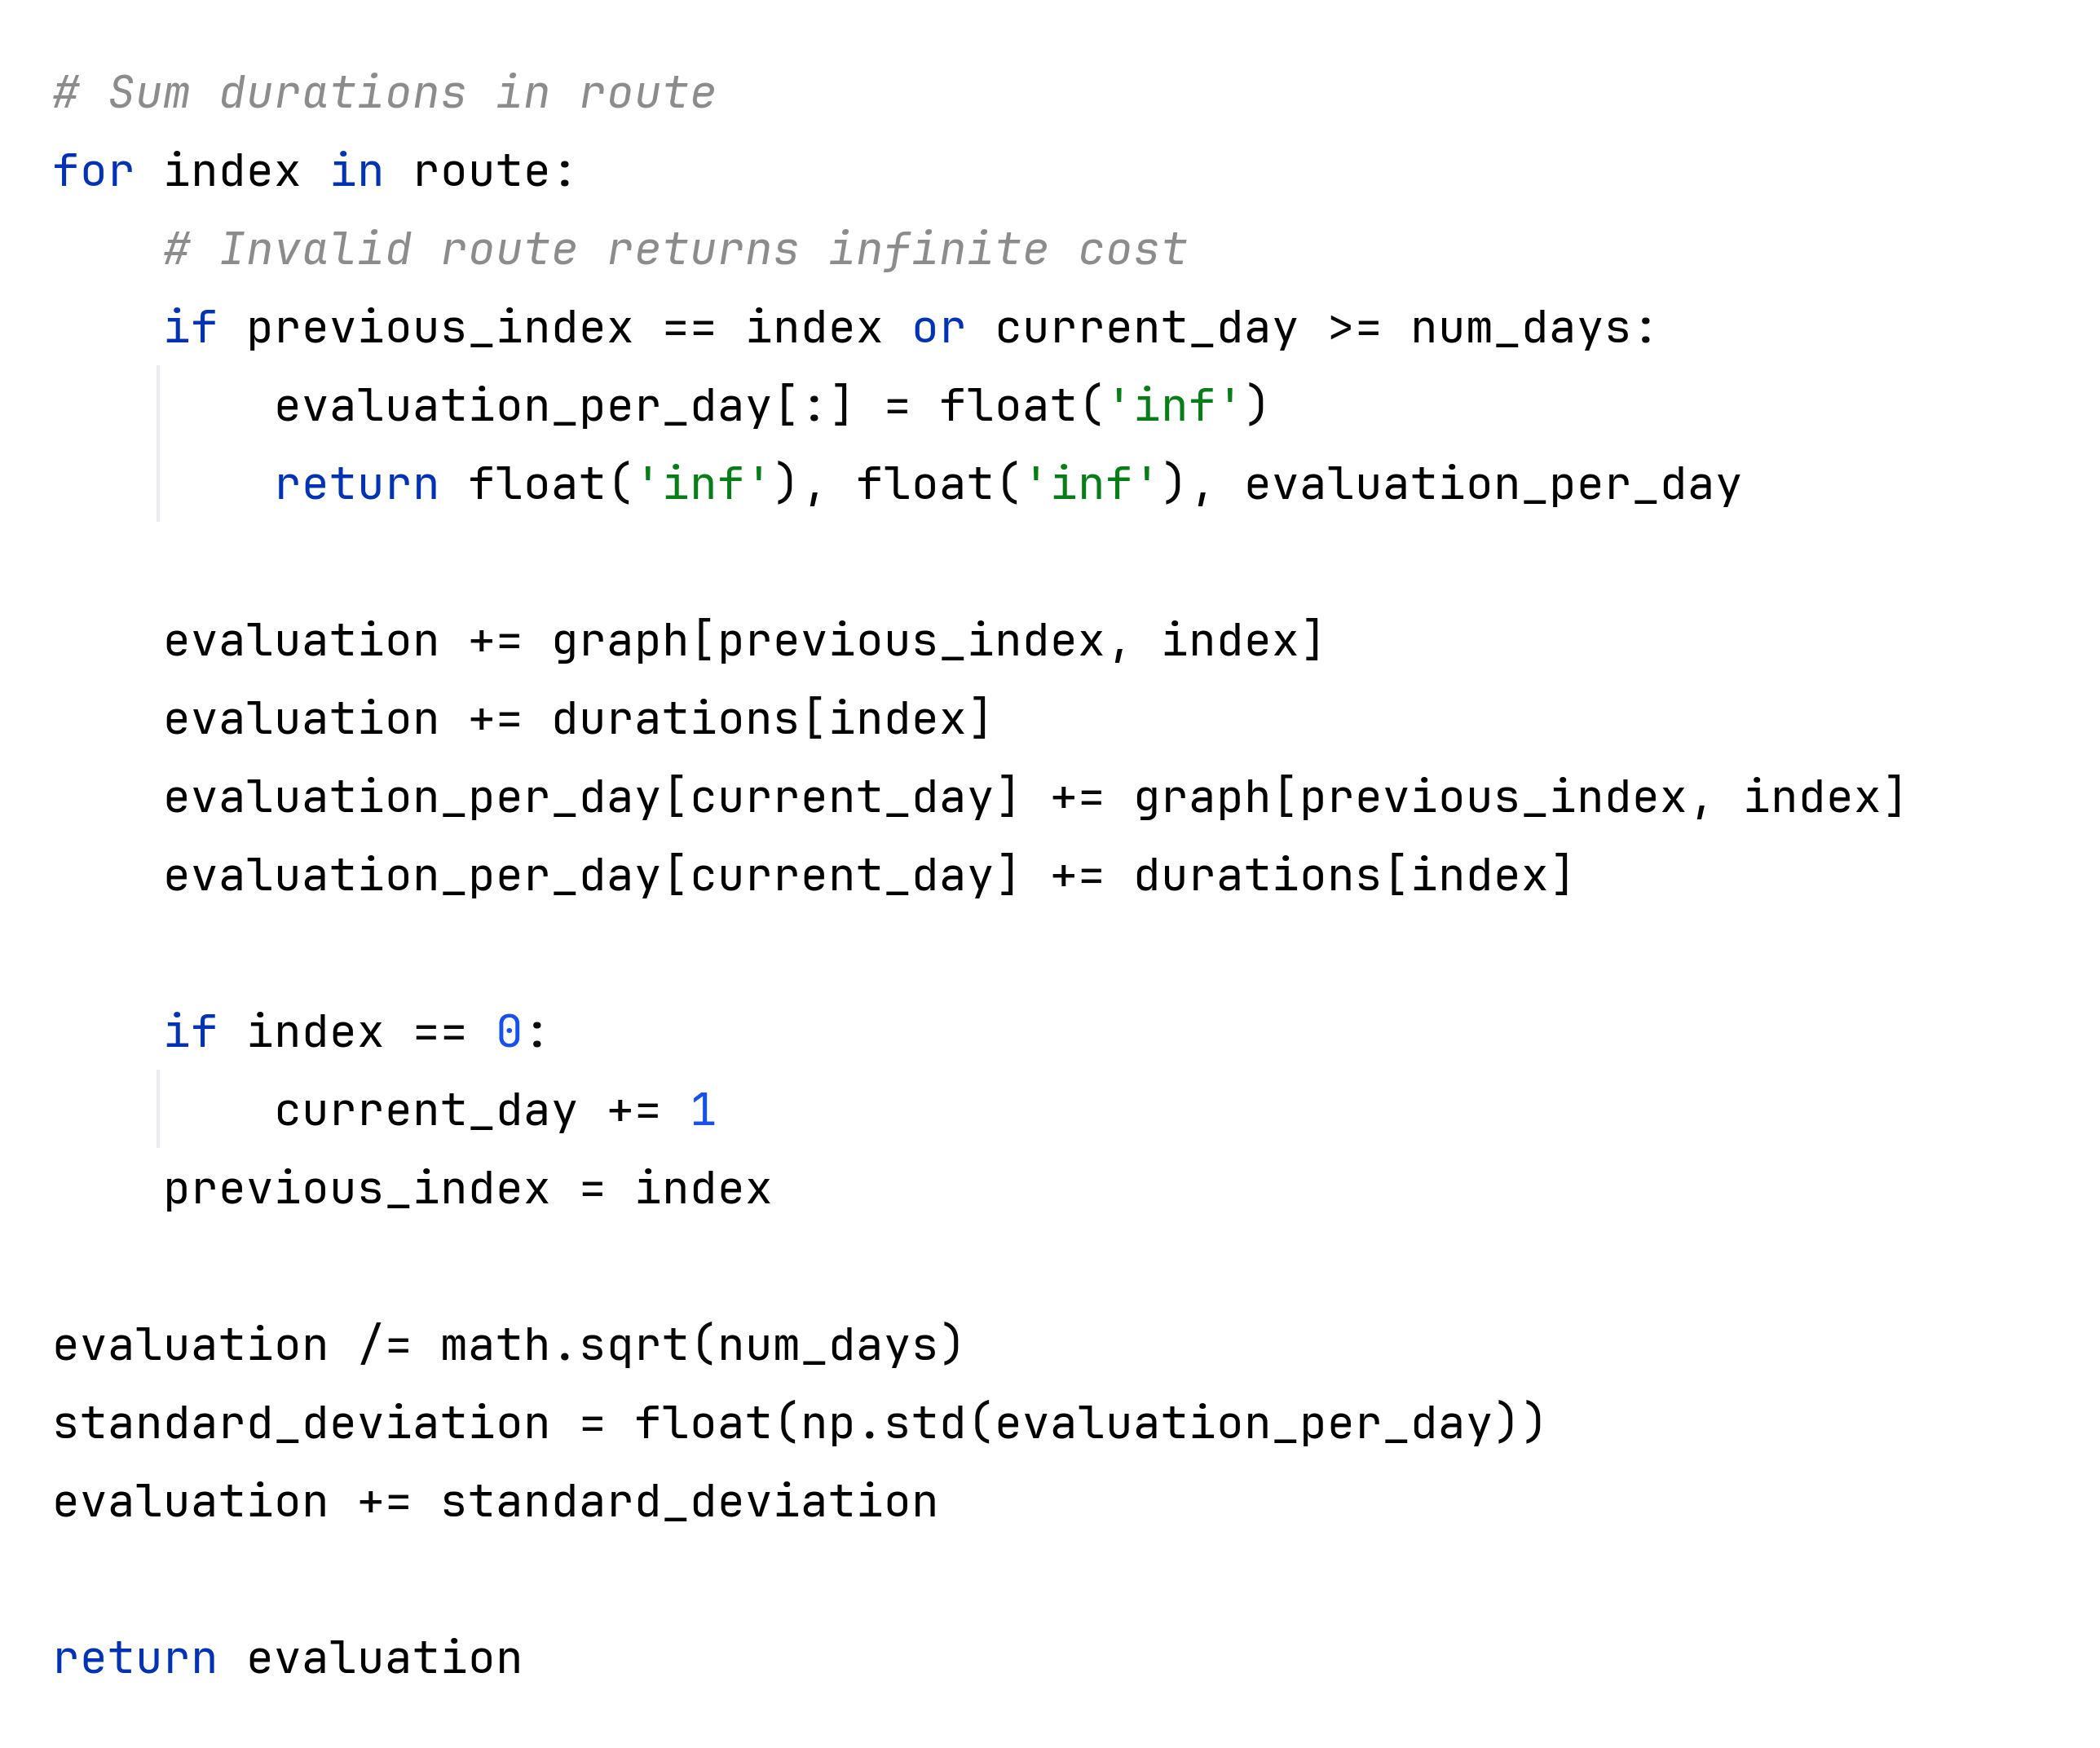
\includegraphics[width = \textwidth]{Algorithm.evaluate_route}
    \caption{Code from Algorithm.evaluate\_route in algorithms\textbackslash algorithm.py}
    \label{fig:Algorithm.evaluate_route}
\end{figure}

\subsection{Clustering}\label{subsec:clustering}
Clustering as a concept can be described as the `organization of a collection of patterns (usually represented as a
vector of measurements, or a point in a multidimensional space) into clusters based on similarity'~\parencite[p. 265]{jain1999data}.
For this problem, clustering will be used to group locations together to form an itinerary for each day of the trip.
These clusters, or days, will then be used as an input for some routing algorithm, which will try and find an
optimal route for each day, which can then be combined to form a complete trip.
Here, the goal of clustering algorithms is to find a set of clusters that, when combined with some routing algorithm,
will produce a trip with minimal cost.
The code in figure~\ref{fig:Clustering.find_route_from_clusters} shows how a set of clusters can be used alongside
graph and duration inputs to find a trip.
\begin{figure}[H]
    \centering
    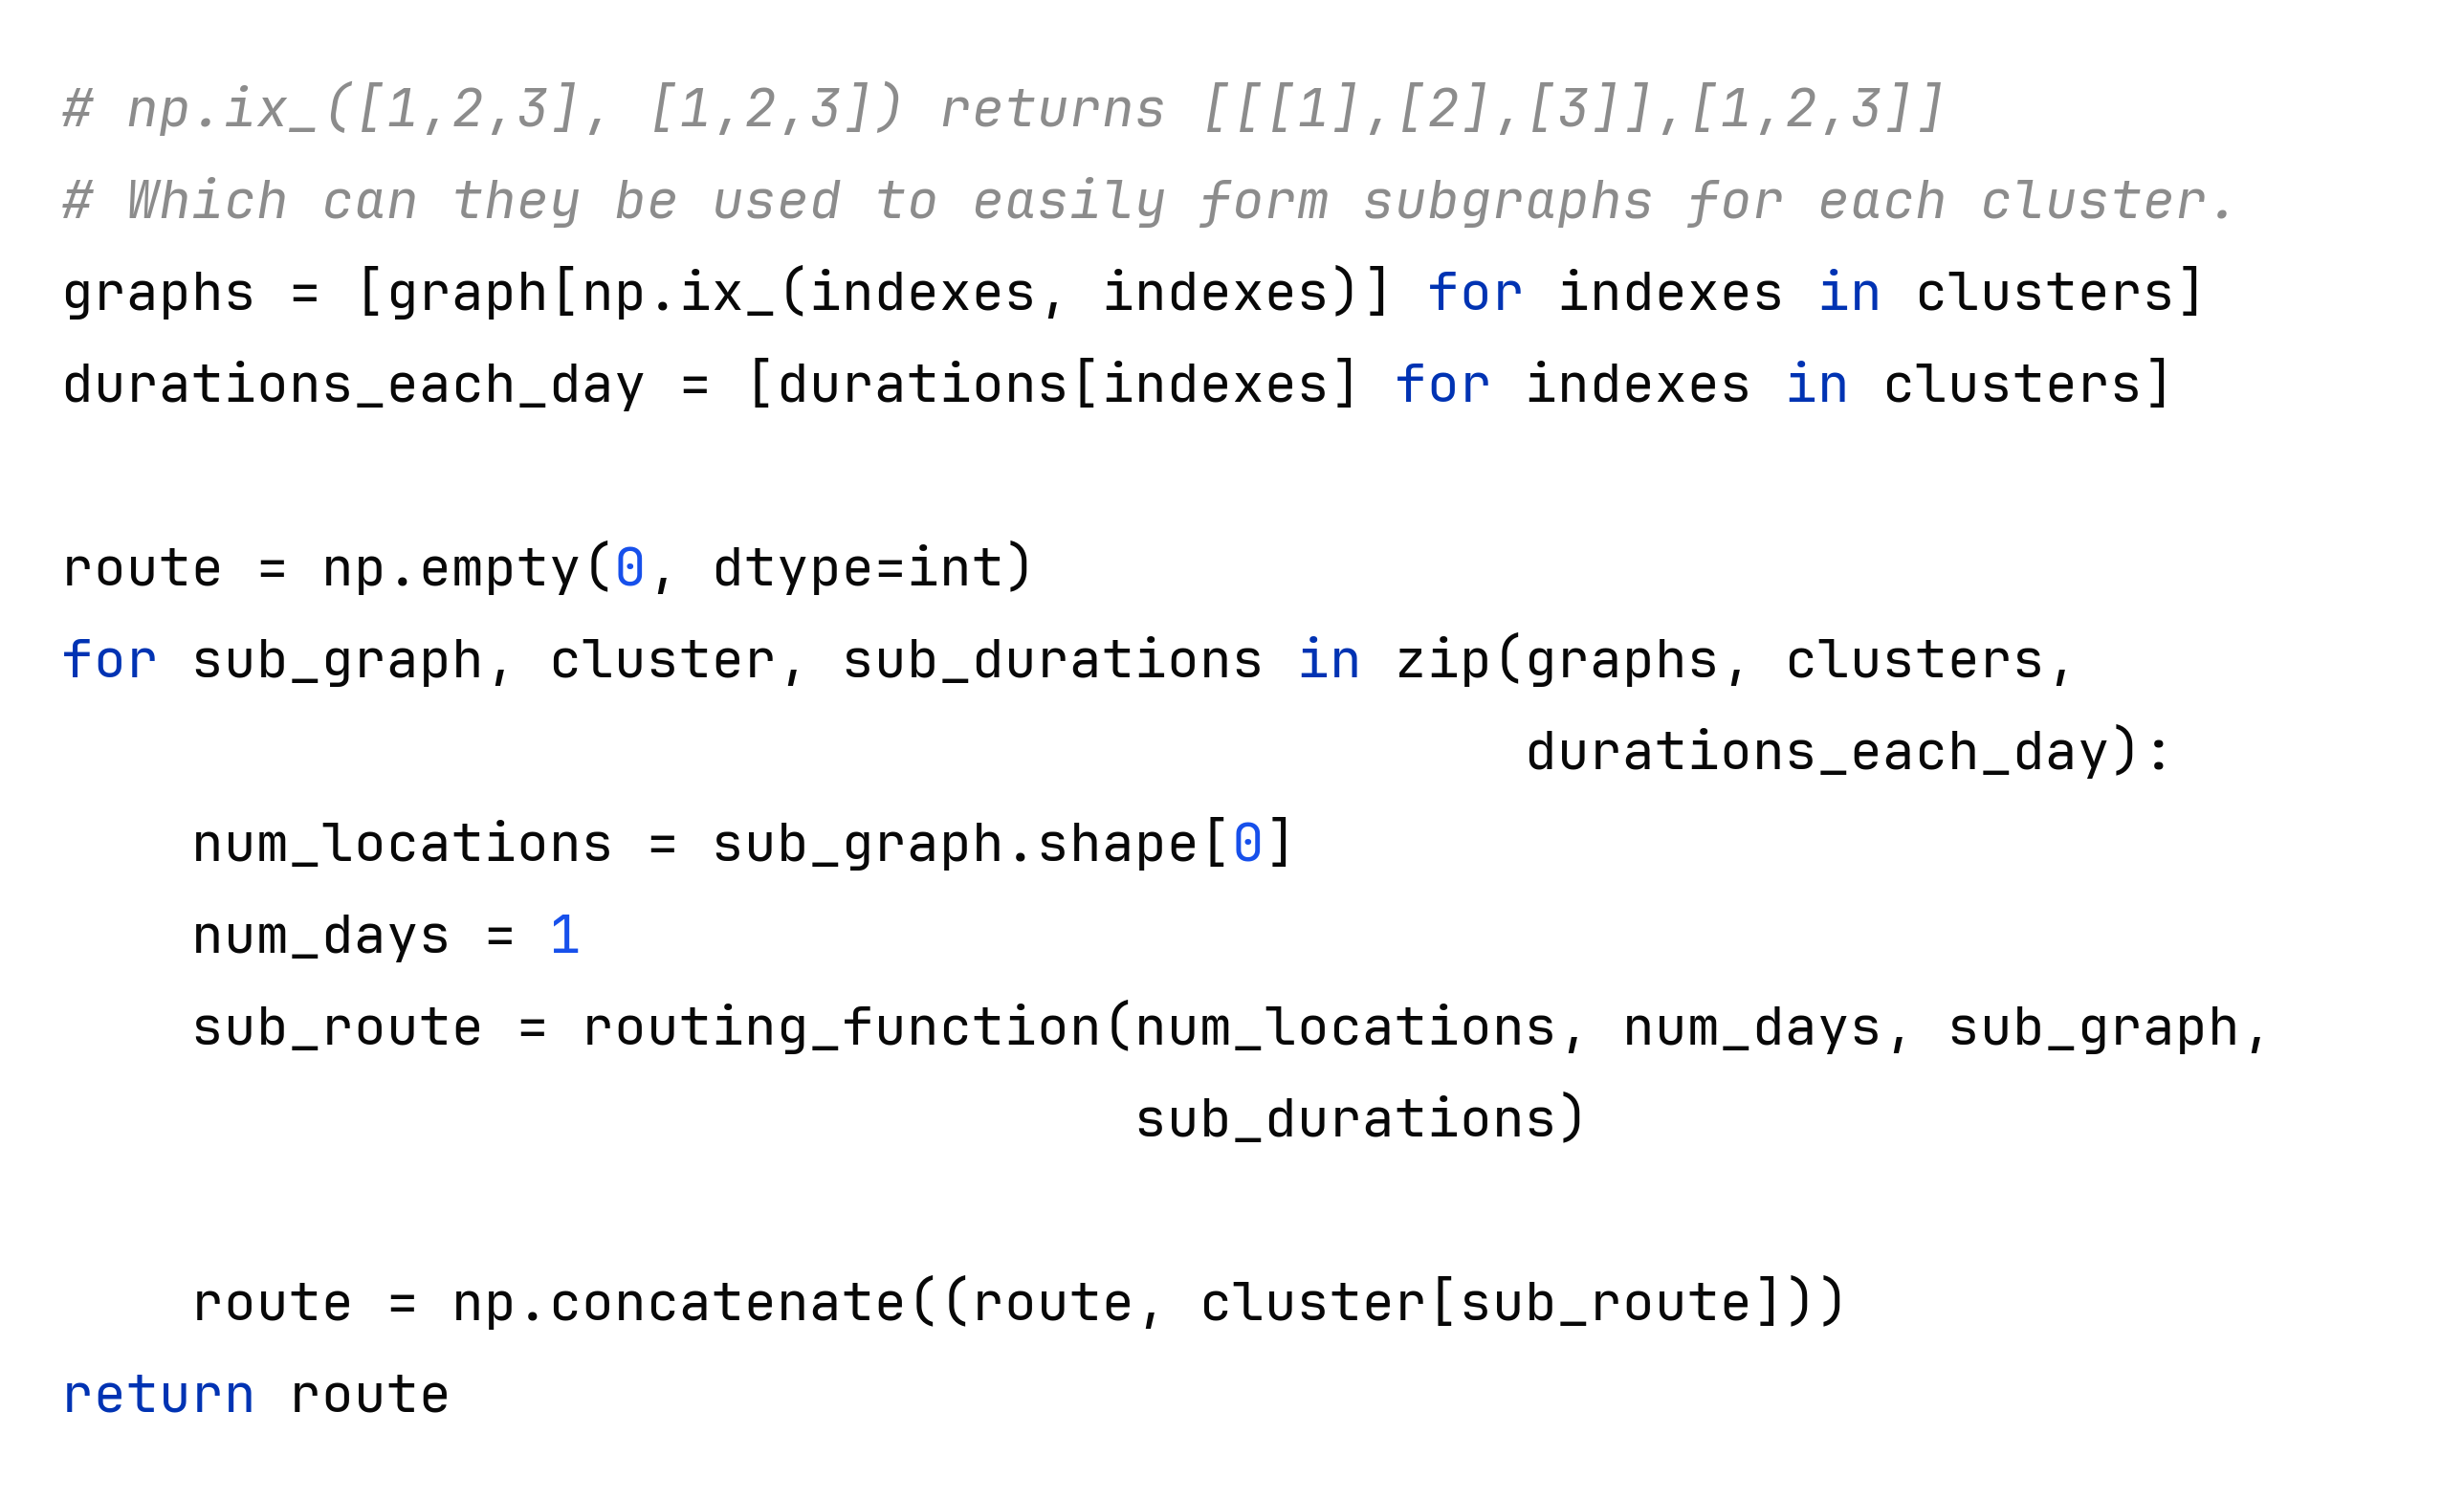
\includegraphics[width = \textwidth]{Clustering.find_route_from_clusters}
    \caption{Code from Clustering.find\_route\_from\_clusters in algorithms\textbackslash clustering.py}
    \label{fig:Clustering.find_route_from_clusters}
\end{figure}

\noindent
The clustering algorithms implemented in this project are: K-Means, Genetic Clustering and Genetic Centroid-based
Clustering.

\subsubsection{K-Means Clustering}\label{subsubsec:k-means}
K-Means is an iterative clustering algorithm that defines its clusters using a set of centroids (means) which are
given a location in the input space, a given location is assigned to the cluster of the `closest' centroid.
The algorithm starts by initialising random centroids and iteratively improving the clustering from there, continuing
until the algorithm converges (on a local optimum) or an iteration limit is reached.
K-Means runs in linear time with a time complexity of $O(m n k i)$, where $m$ is the number of locations, $n$ is the
dimensionality of the input, $k$ is the number of clusters, and $i$ is the number of iterations~\parencite[p. 102]{hartigan1979algorithm}.
The inputs will always contain only two dimensions, and a maximum number of iterations will be set, making both $n$ and
$i$ constants, allowing the simplification of the time complexity to $O(m k)$.\\

\noindent
In this implementation of K-Means centroids will be initialised by randomly selecting unique locations from the input,
and placing the initial centroids at their coordinates.
A different approach was considered, which involved initialising the centroids with random coordinates in a similar
area to the input, however this had the potential to create clusters with zero locations assigned to them resulting
in invalid trips.
By starting with locations from the input, there is certainty that all clusters have at least one location assigned to
them.
We will be the coordinates of inputted locations will be used to calculate the Euclidean distances between locations
and centroids, these locations are then assigned to the cluster of the closest centroid.
Figure~\ref{fig:Clustering._assign_nodes_to_centroid} shows how this was accomplished.
\begin{figure}[H]
    \centering
    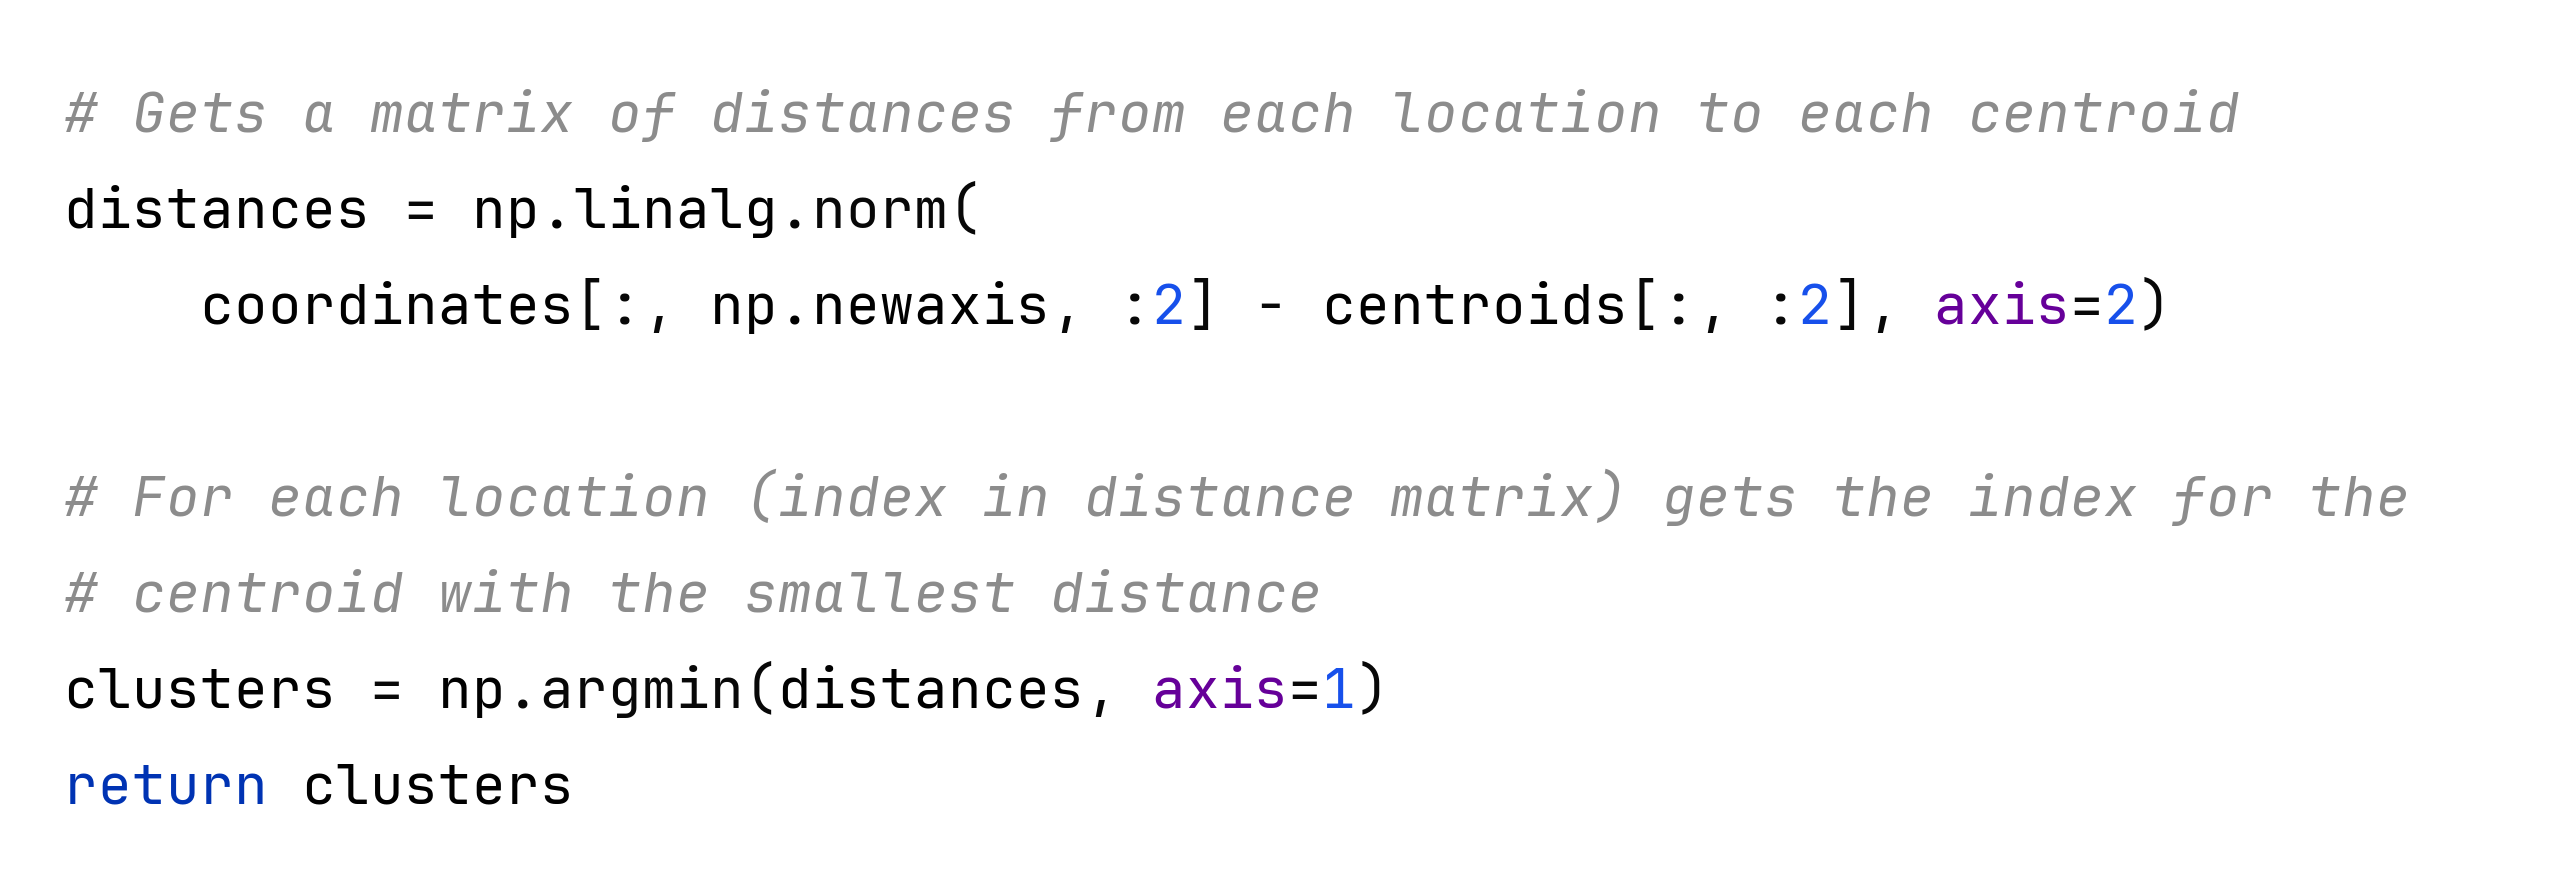
\includegraphics[width = \textwidth]{Clustering._assign_nodes_to_centroid}
    \caption{Code from Clustering.\_assign\_nodes\_to\_centroid in algorithms\textbackslash clustering.py}
    \label{fig:Clustering._assign_nodes_to_centroid}
\end{figure}

\noindent
After assignment, the centroids are recalculated such that their coordinates are the average of all locations
assigned to their cluster.
This is done by iterating through each cluster and calculating the mean of all locations assigned to it.
The implementation of this is shown in figure~\ref{fig:KMeans._compute_means}.
\begin{figure}[H]
    \centering
    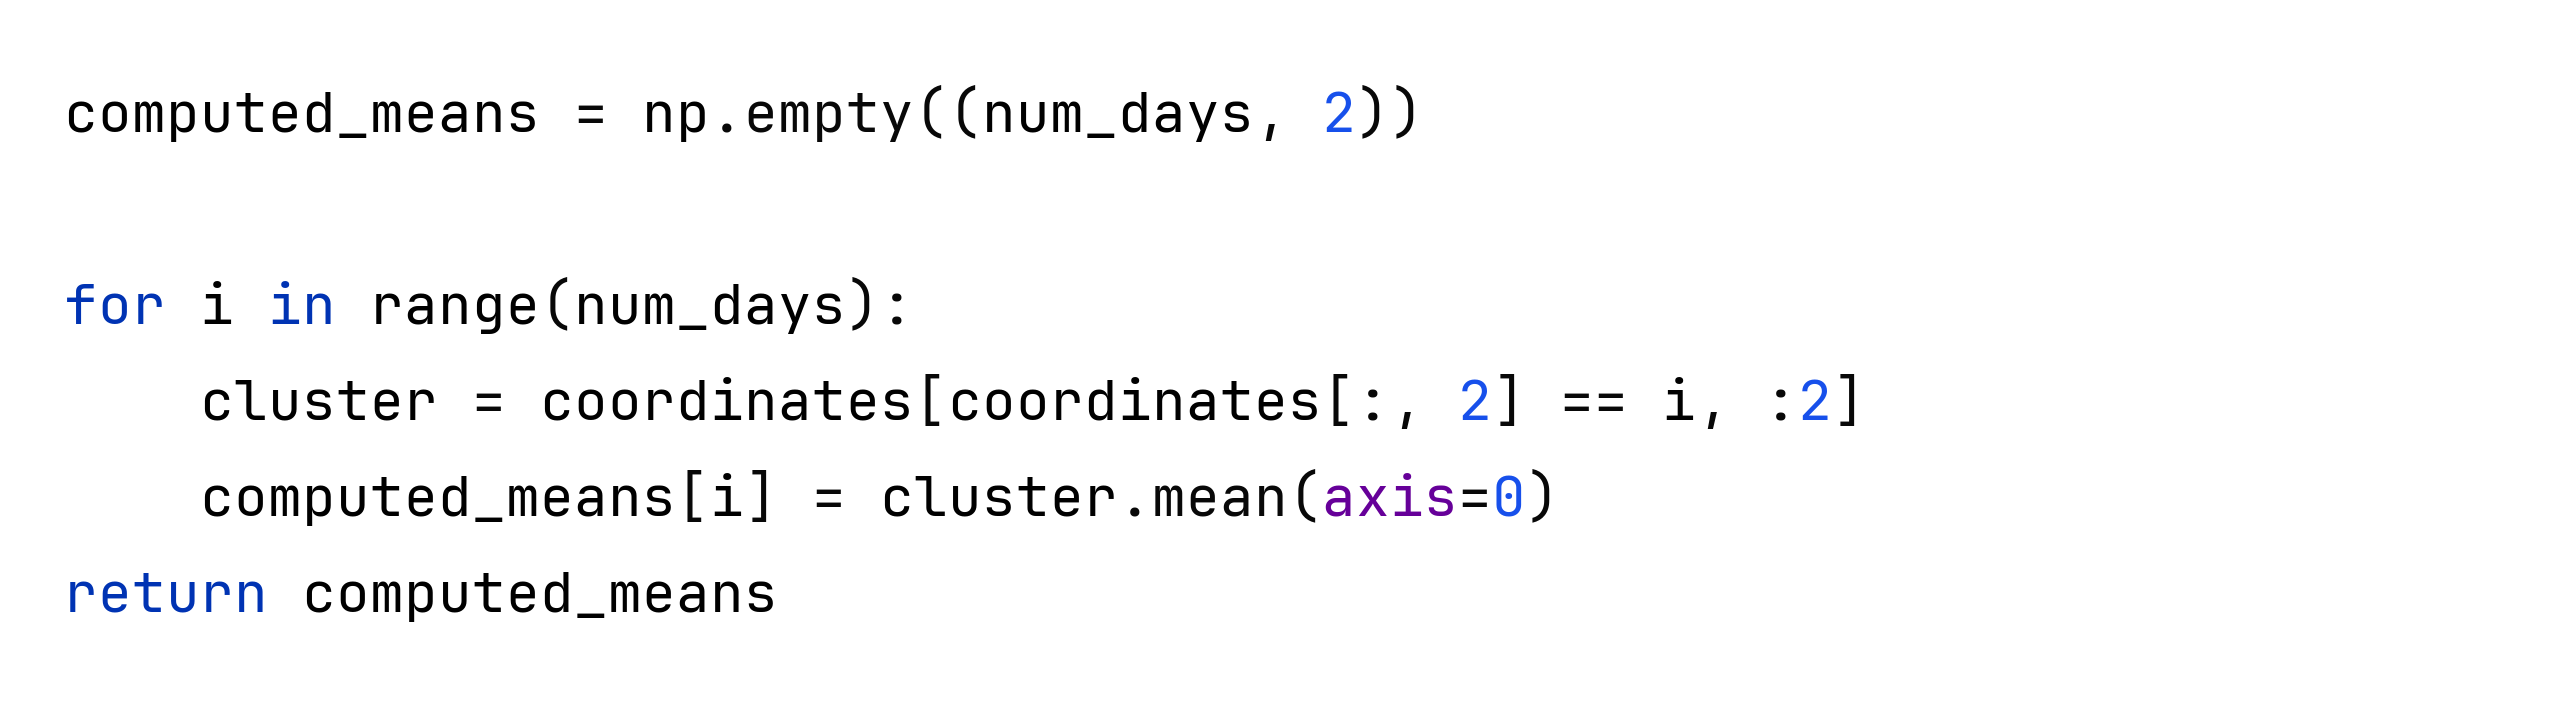
\includegraphics[width = \textwidth]{KMeans._compute_means}
    \caption{Code from KMeans.\_compute\_means in algorithms\textbackslash clustering.py}
    \label{fig:KMeans._compute_means}
\end{figure}

\noindent
These steps of cluster assignment and centroid recalculation are repeated until either a maximum allowed number of
iterations is reached, or until the algorithm converges on an optimum solution.
The convergence criterion is that the centroids stop changing between iterations, i.e., the centroids are the same
as the previous iteration.
The python implementation of this is shown in figure~\ref{fig:KMeans.find_clusters}.
\begin{figure}[H]
    \centering
    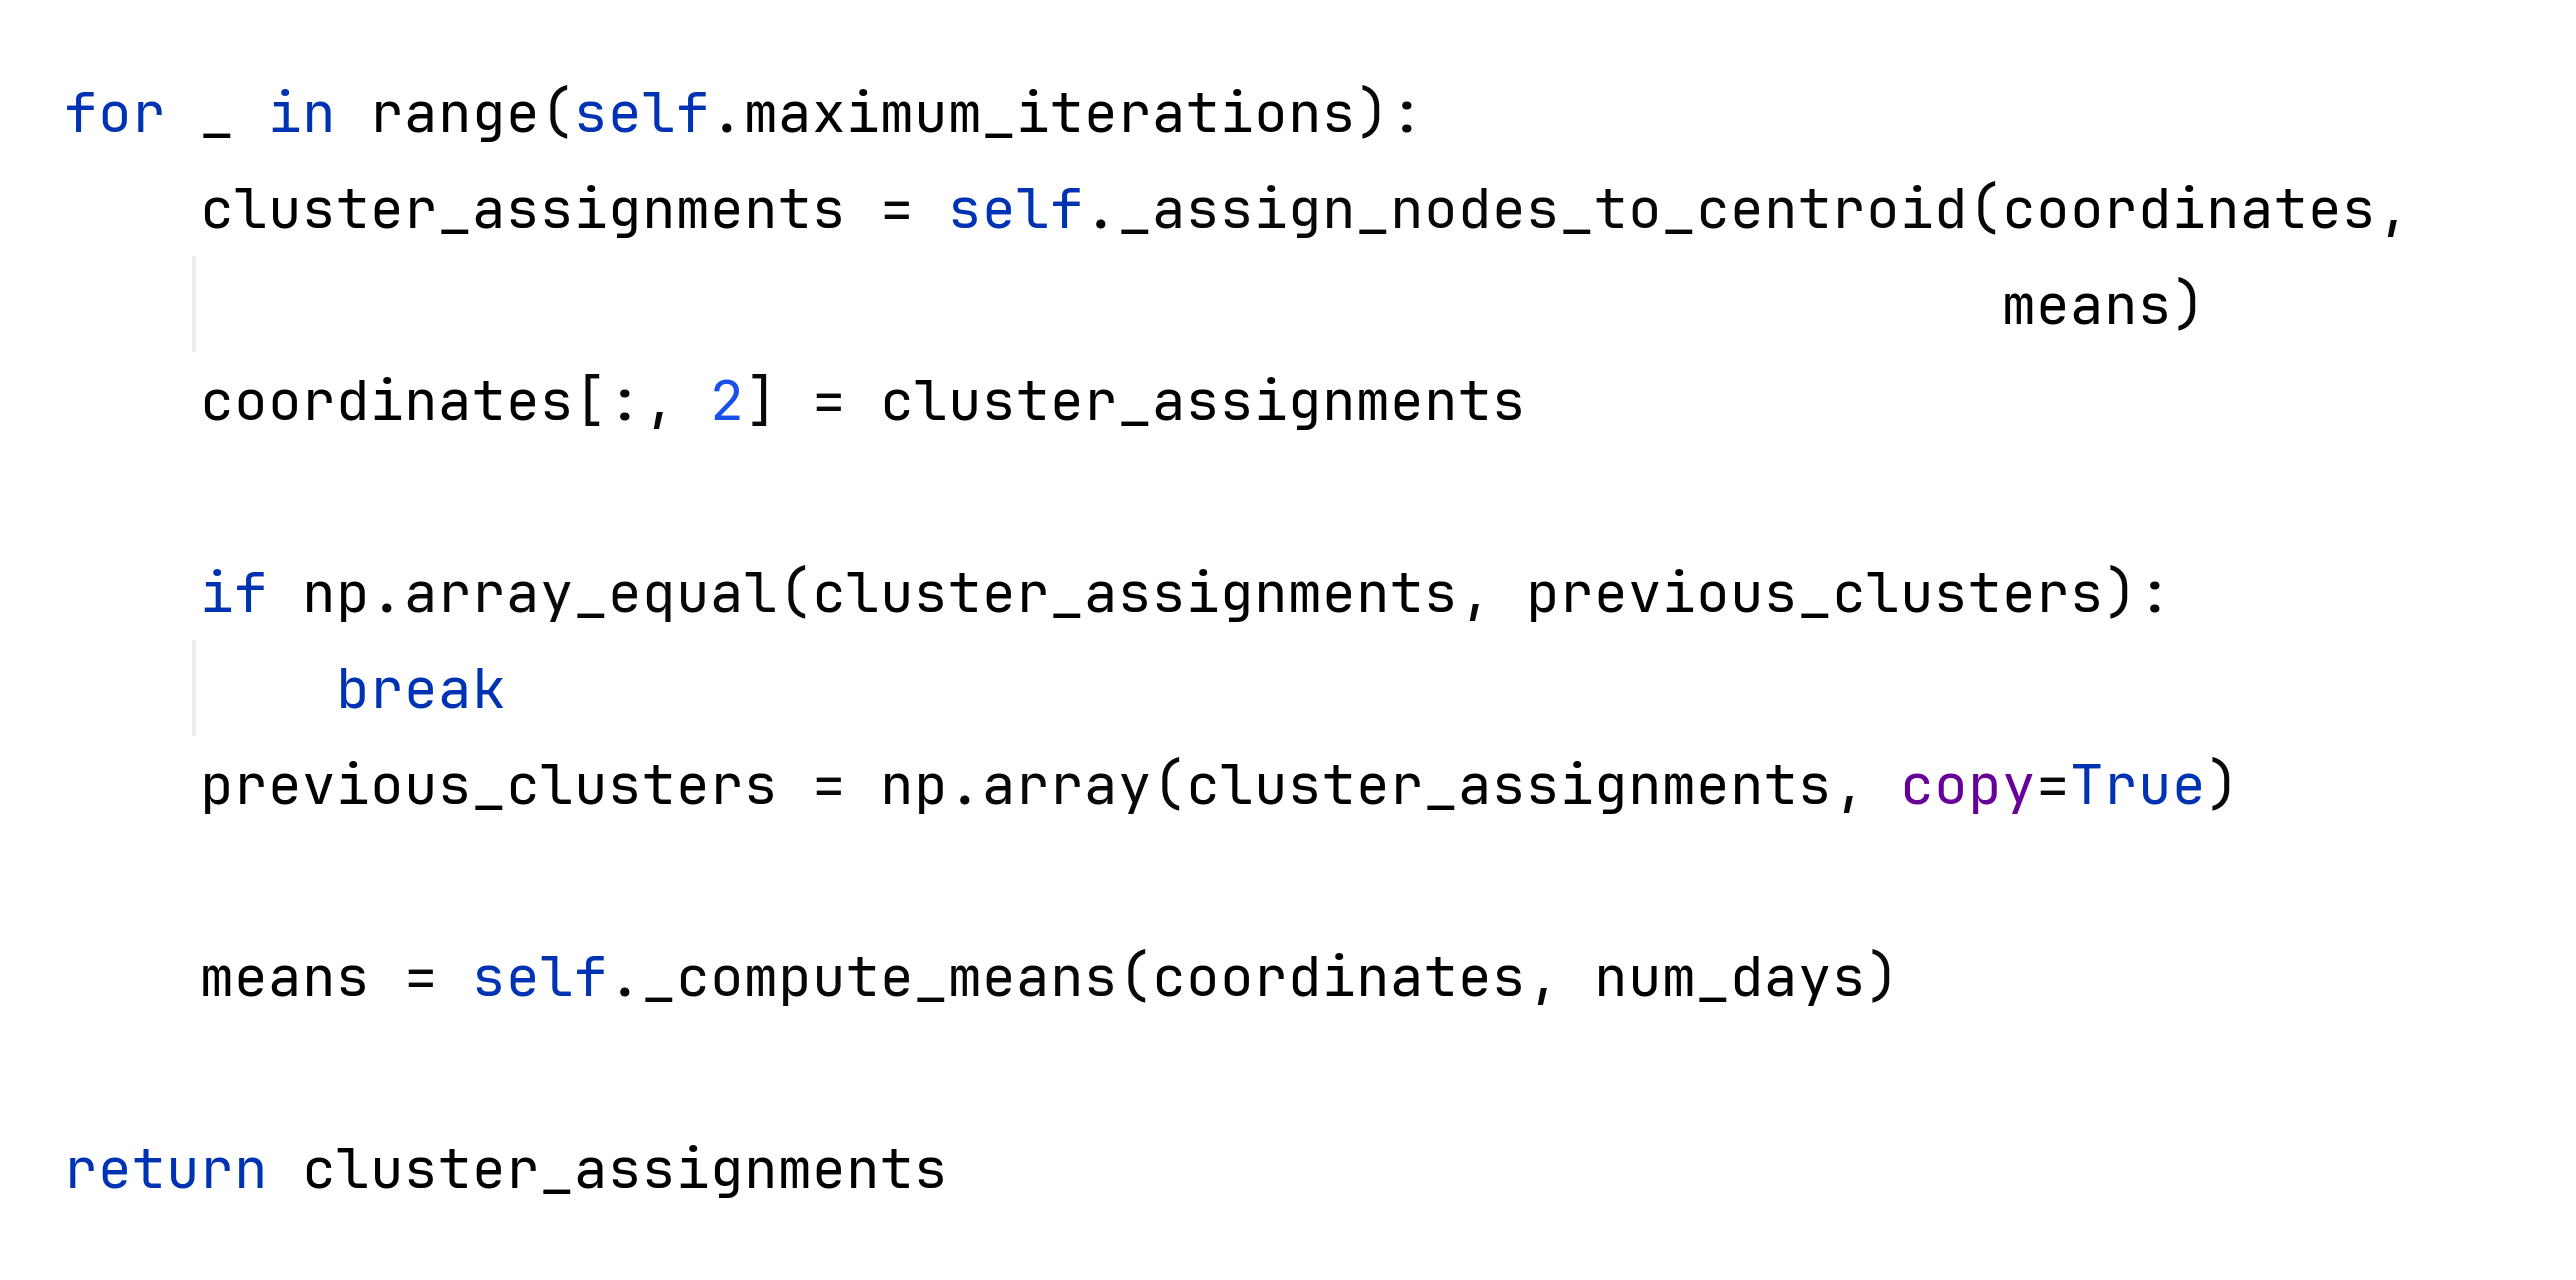
\includegraphics[width = \textwidth]{KMeans.find_clusters}
    \caption{Code from KMeans.find\_clusters in algorithms\textbackslash clustering.py}
    \label{fig:KMeans.find_clusters}
\end{figure}

\noindent
Figure~\ref{fig:KMeans_London_Step1} shows an example of the iterations of a K-Means algorithm run on an input with
12 points of interest around London to be visited over 3 days.
\begin{figure}[H]
    \ContinuedFloat*
    \centering
    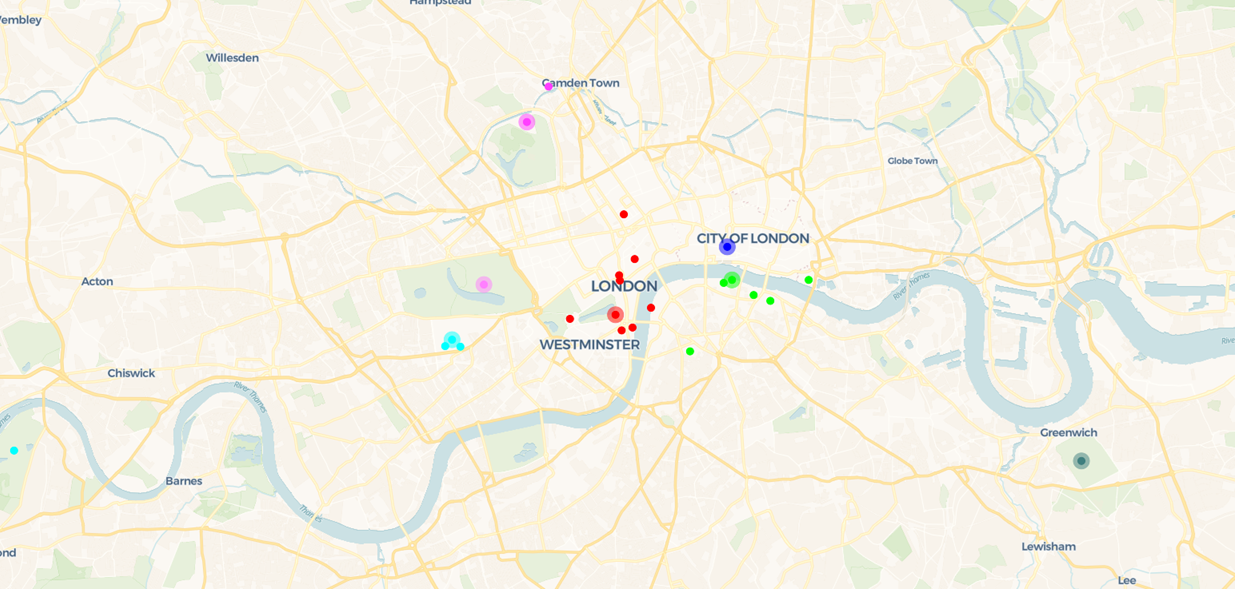
\includegraphics[width = \textwidth]{KMeans_London_Step1}
    \caption{K-Means example Step 1, Initial centroid positions and cluster assignments.}
    \label{fig:KMeans_London_Step1}
\end{figure}
\begin{figure}[H]
    \ContinuedFloat
    \centering
    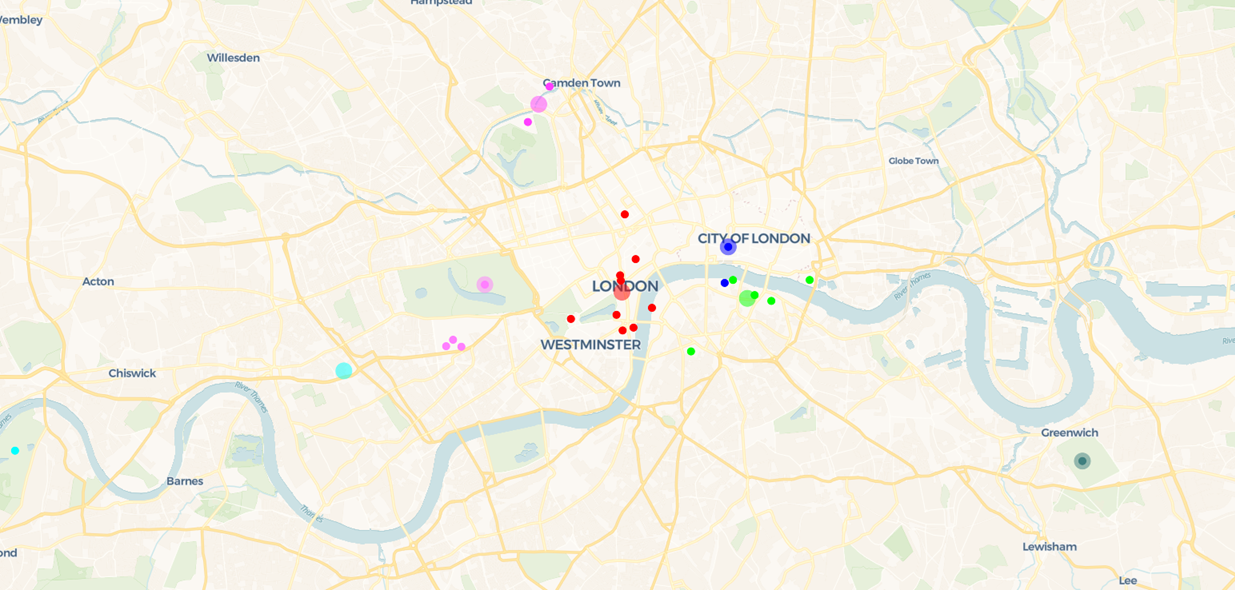
\includegraphics[width = \textwidth]{KMeans_London_Step2}
    \caption{K-Means example Step2, Centroids have been updated, locations are reassigned to their closest centroid.}
    \label{fig:KMeans_London_Step2}
\end{figure}
\begin{figure}[H]
    \ContinuedFloat
    \centering
    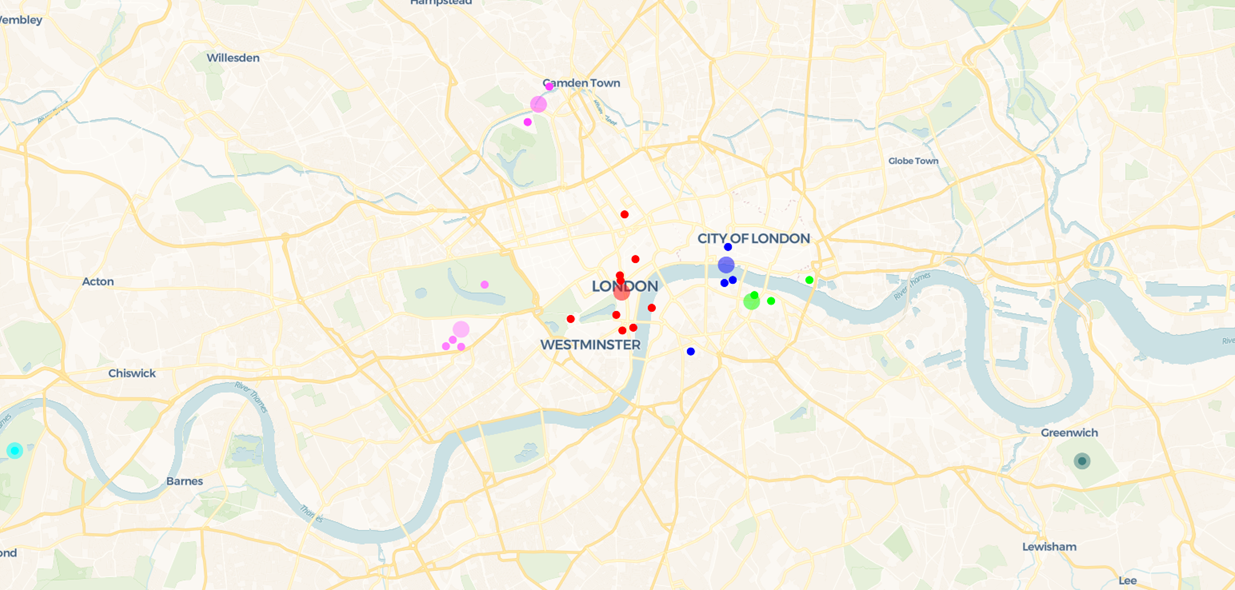
\includegraphics[width = \textwidth]{KMeans_London_Step3}
    \caption{K-Means example Step3, Centroids have updated and no locations have changed cluster, a solution has been found.}
    \label{fig:KMeans_London_Step3}
\end{figure}

\noindent
It is worth noting that K-Means only forms these clusters based on Euclidean distances, grouping together locations
that are close geographically.
However, as formally described in the \hyperref[subsec:objective-function]{Objective Function} section of the
\hyperref[sec:problem-formulation]{Problem Formulation}, a good trip will minimise both the route length of the trip
and the variance between time spent each day.
K-Means does not aim to optimise for the variance between days, it fails to consider the time spent at each
location.
Furthermore, while each cluster might be optimised for distance, how close two locations are may not reflect the travel
time between them.
While K-Means does not intentionally optimise for variance between days or consider travel time between locations, it
was still chosen for this project out of curiosity as to how effective a heuristic it might provide.
Hopefully it will offer a simple and computationally efficient baseline for comparison with more complex
algorithms.

\subsubsection{Genetic Clustering}
Genetic clustering applies genetic algorithms to attempt and find the best assignment of locations to clusters.
Genetic algorithms are a type of evolutionary algorithm that aims to mimic biological evolution to find an optimal
solution.
They involve creating a population of potential solutions (individuals) and iteratively improving the population
through selection (keeping the best individuals in the population, akin to natural selection), crossover (combining
individuals to create offspring, akin to sexual reproduction), and mutation (randomly altering the genomes
of individuals in the population, akin to biological mutation).

To perform selection, and find the best solutions in a population, each individual requires some fitness assigned to it.
To calculate this fitness cluster assignments will be combined with a chosen routing algorithm, and a cost function
applied to the route found.
This cost will be used to rank a population, assisting in the identification of clusters that can produce a good trip.

The performance of Genetic algorithms is highly dependent on its hyperparameters: mutation rate, determining how
common mutation is; crossover rate, determining how often offspring are created via crossover, as opposed to new
additions to the population; population size, determining how many individuals there are per generation; number of
generations, determining how many generations will be evolved to reach a solution; crossover method used,
determining how crossover is performed to create offspring; and in this case, the routing algorithm used, which may
impact how clusters are used to form routes.
These hyperparameters impact both the runtime of the algorithm and the exploration of the search space, indirectly
impacting the quality of the solution.
For each generation, Genetic Clustering has to route and evaluate each individual in the population, yielding a time
complexity of $O(g p r n)$, with $g$ being the number of generations, $p$ being the population size,
$r$ being the time complexity of the chosen routing algorithm and $n$ being the number of locations and days.\\

\noindent
For this Genetic Clustering implementation, an individual is represented by a genome, which will provide a mapping
that assigns each location to a cluster.
Figure~\ref{fig:barcelona-genome-example} shows an example of this.
\begin{figure}[H]
    \centering
    Genome: [0, 0, 0, 1, 1, 1, 2, 2, 2]\\
    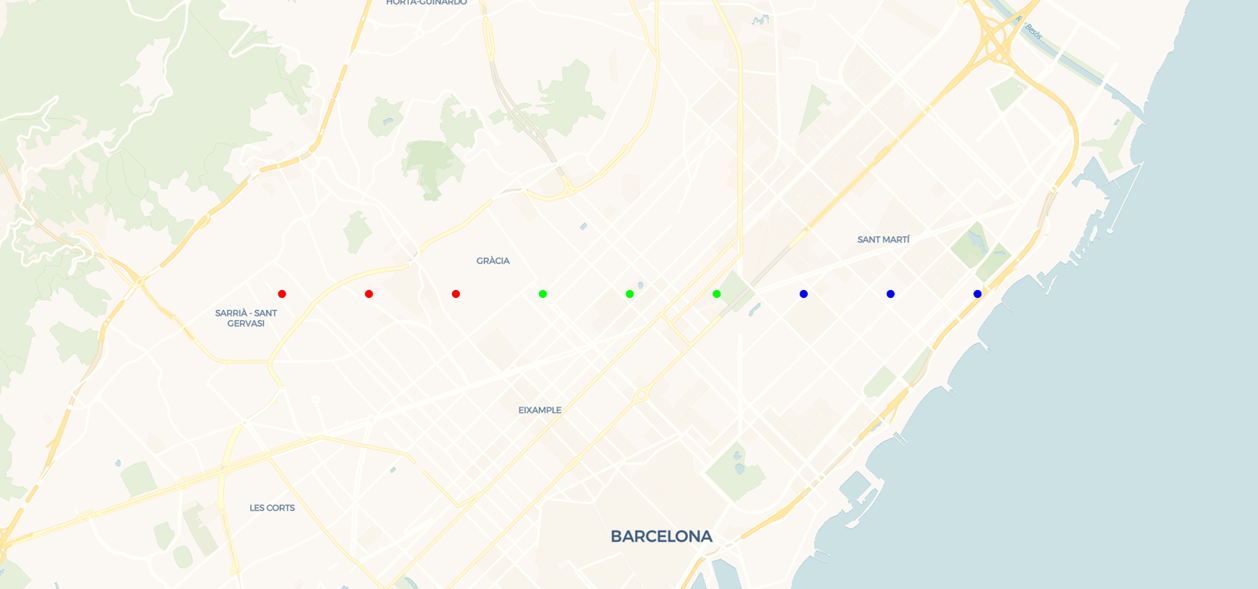
\includegraphics[width = \textwidth]{Barcelona_Genome_Example}
    \caption{Example of how an individual's genome corresponds to cluster assignments.}
    \label{fig:barcelona-genome-example}
\end{figure}

\noindent
These genomes are the target for performing crossover and mutations.
We begin this evolution process by randomly generating an initial population of individuals.
From there, following steps are repeated until reach a maximum number of generations is reached:
\begin{enumerate}
    \item Evaluation of the fitness of each individual in the population.
    \item Selection of the best individuals from the population, these will be carried over into the next generation, as
    well as be used to create offspring.
    \item Creation of the new population using crossover and mutation.
\end{enumerate}

\noindent
As previously discussed, the fitness of each individual is evaluated by applying a routing algorithms to the
clusters defined by the genome, and then applying the cost function to the resulting route.
Figure~\ref{fig:GeneticClustering._evaluate_population} shows this route finding and evaluation.
\begin{figure}[H]
    \centering
    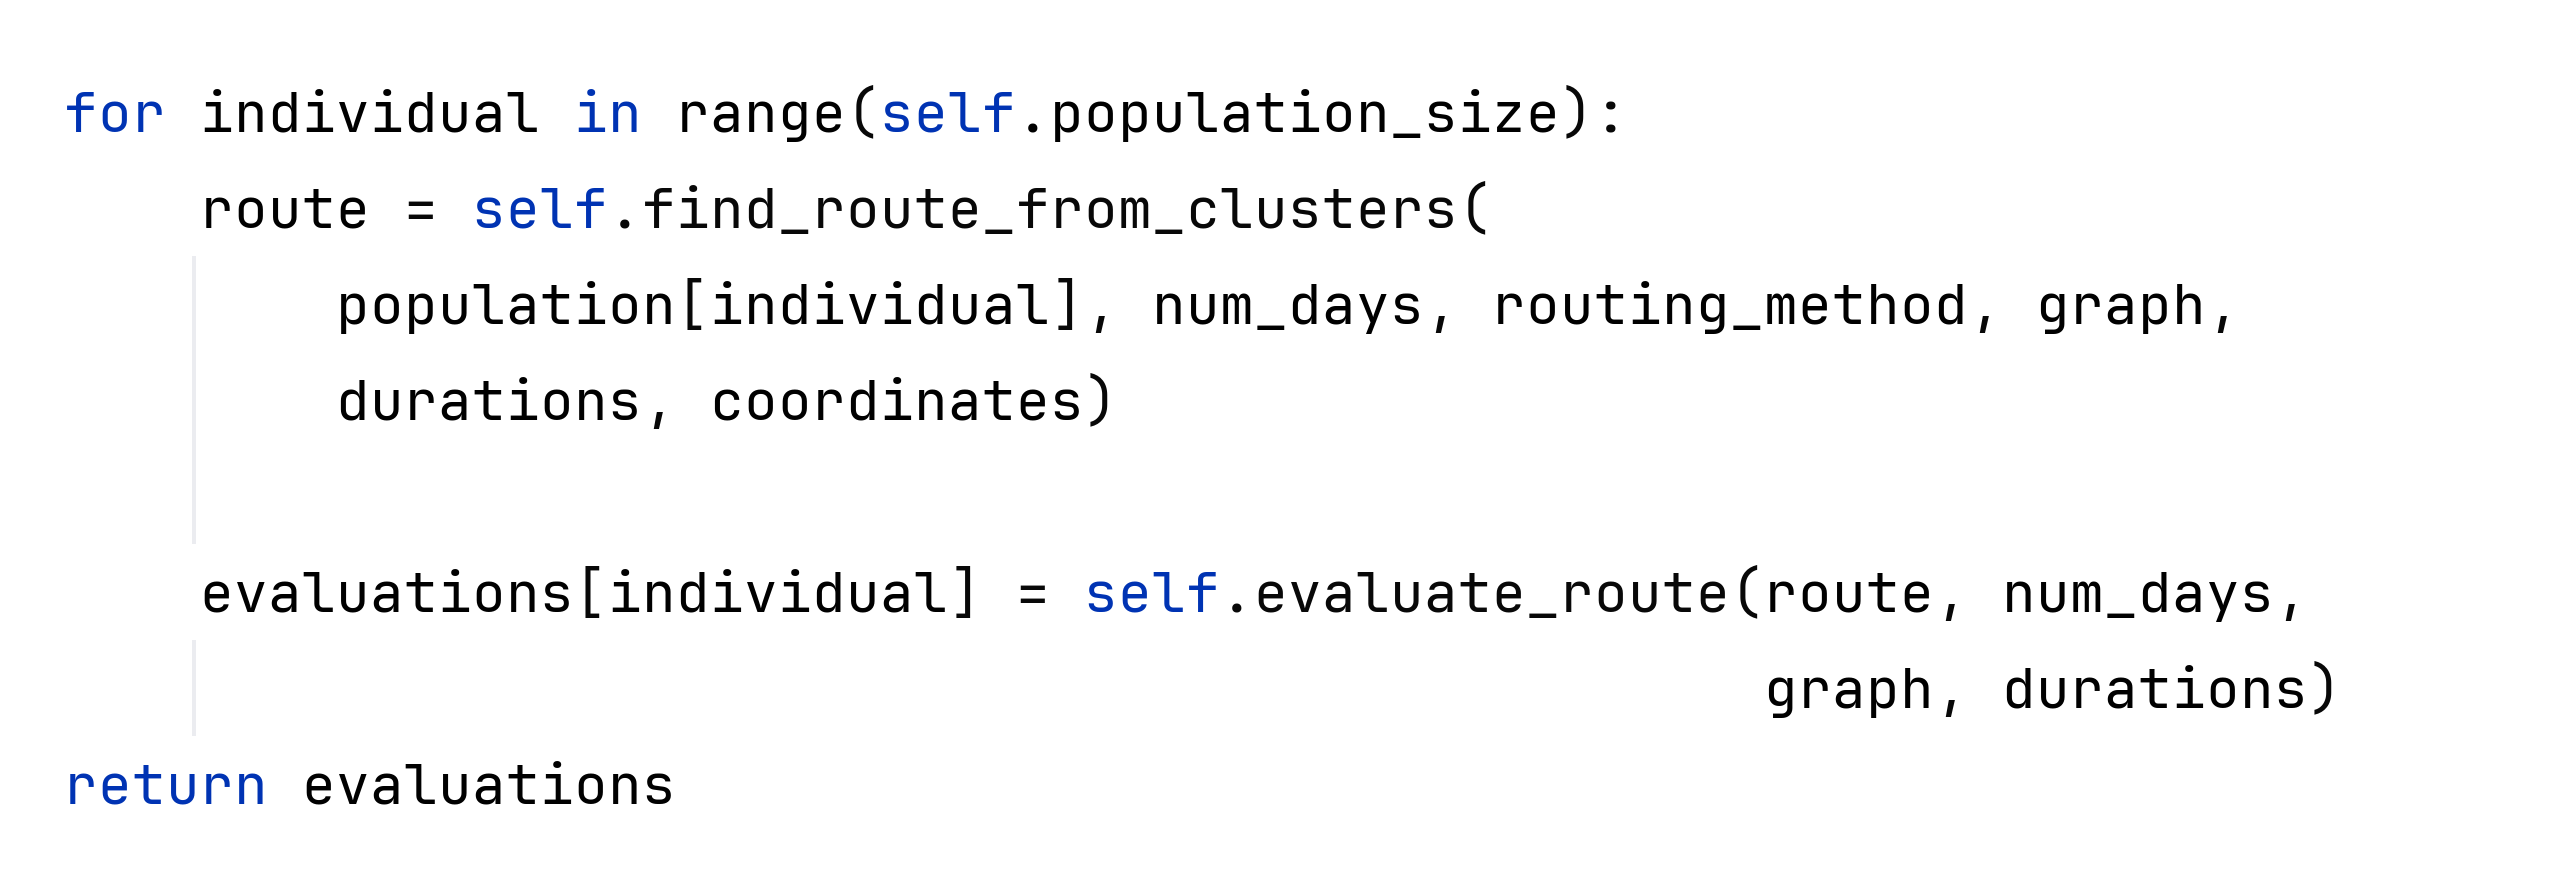
\includegraphics[width = \textwidth]{GeneticClustering._evaluate_population}
    \caption{Code from GeneticClustering.\_evaluate\_population in algorithms\textbackslash clustering.py}
    \label{fig:GeneticClustering._evaluate_population}
\end{figure}

\noindent
The methods called in figure~\ref{fig:GeneticClustering._evaluate_population} are those previously shown in
figure~\ref{fig:Clustering.find_route_from_clusters} (find\_route\_from\_clusters) and
figure~\ref{fig:Algorithm.evaluate_route} (evaluate\_route).
\textcite{tang2000multiple}'s genetic algorithm featured a selection process involving choosing the best individual for
one parent, with the other parent being selected via a semi-random process with bias based on the performance of each
individual.
For the genetic algorithms implemented in this project, the two best individuals of a population will be chosen as
parents, without any random selection.
Figure~\ref{fig:GeneticClustering.find_clusters.select_parents} shows this simple selection process in python.
\begin{figure}[H]
    \centering
    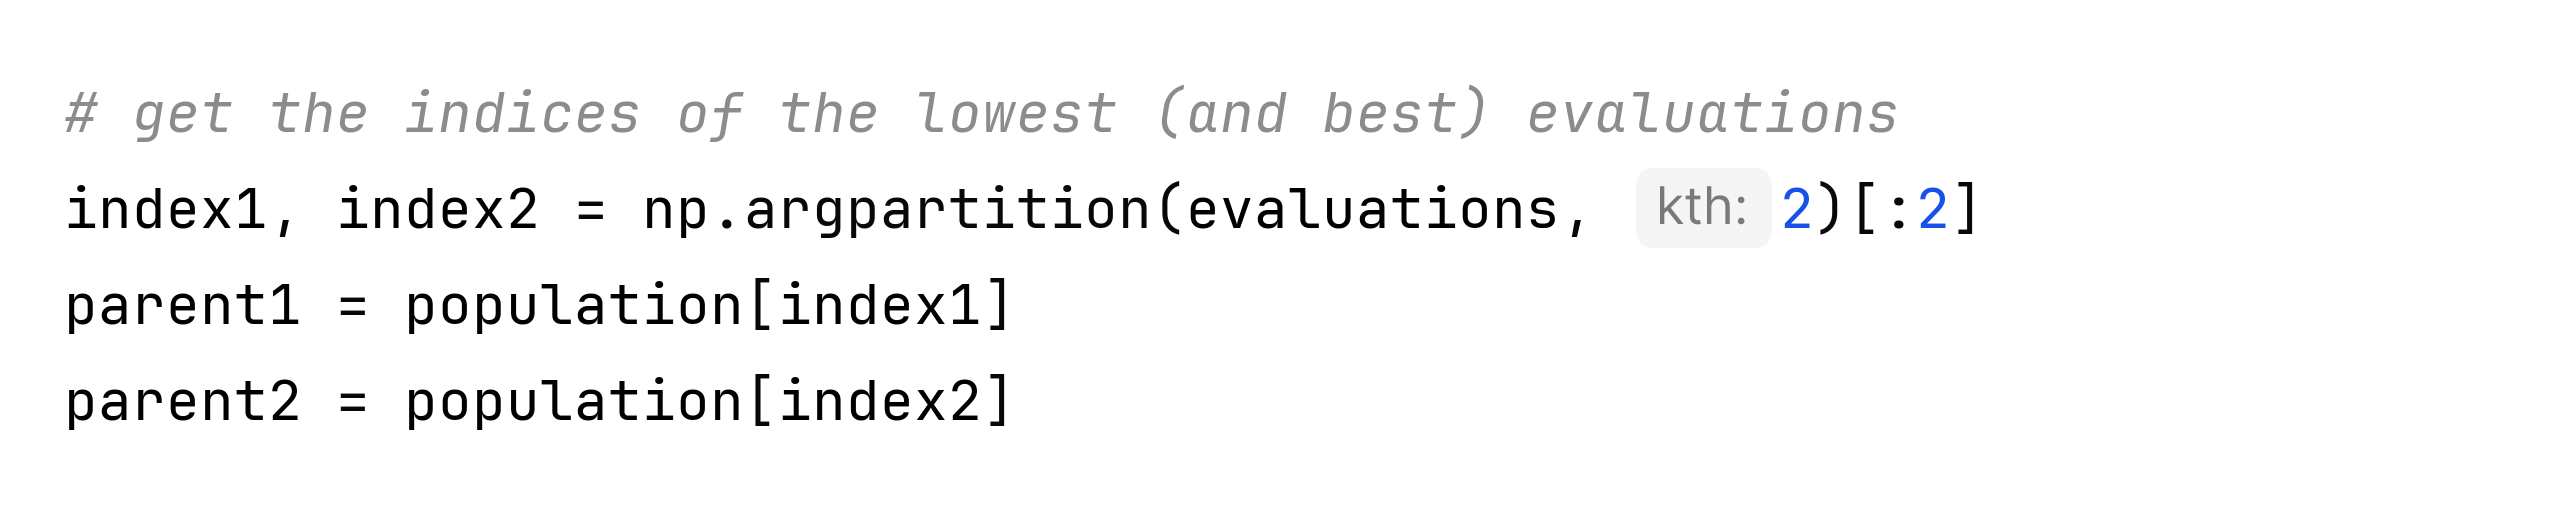
\includegraphics[width = \textwidth]{GeneticClustering.find_clusters.select_parents}
    \caption{Code from GeneticClustering.find\_clusters in algorithms\textbackslash clustering.py}
    \label{fig:GeneticClustering.find_clusters.select_parents}
\end{figure}

\noindent
Excluding the two parents, who will be copied over, the next generation will be created via crossover and mutation,
or through random generation.
By taking the two best individuals as parents, good solutions are likely to be maintained, but will trade off genetic
diversity, perhaps leading the algorithm to get stuck in local optima and not sufficiently exploring the search space.
To counter-act this, and boost the genetic diversity of each population some randomly generated individuals in an effort
to increase genetic diversity and exploration of the search space.
Figure ~\ref{fig:GeneticClustering.find_clusters.crossover} shows how this decision was implemented.
For each individual a random number is generated between 0 and 1, if this number is lower than the crossover rate
the individual is created via crossover, otherwise it will be randomly generated.
\begin{figure}[H]
    \centering
    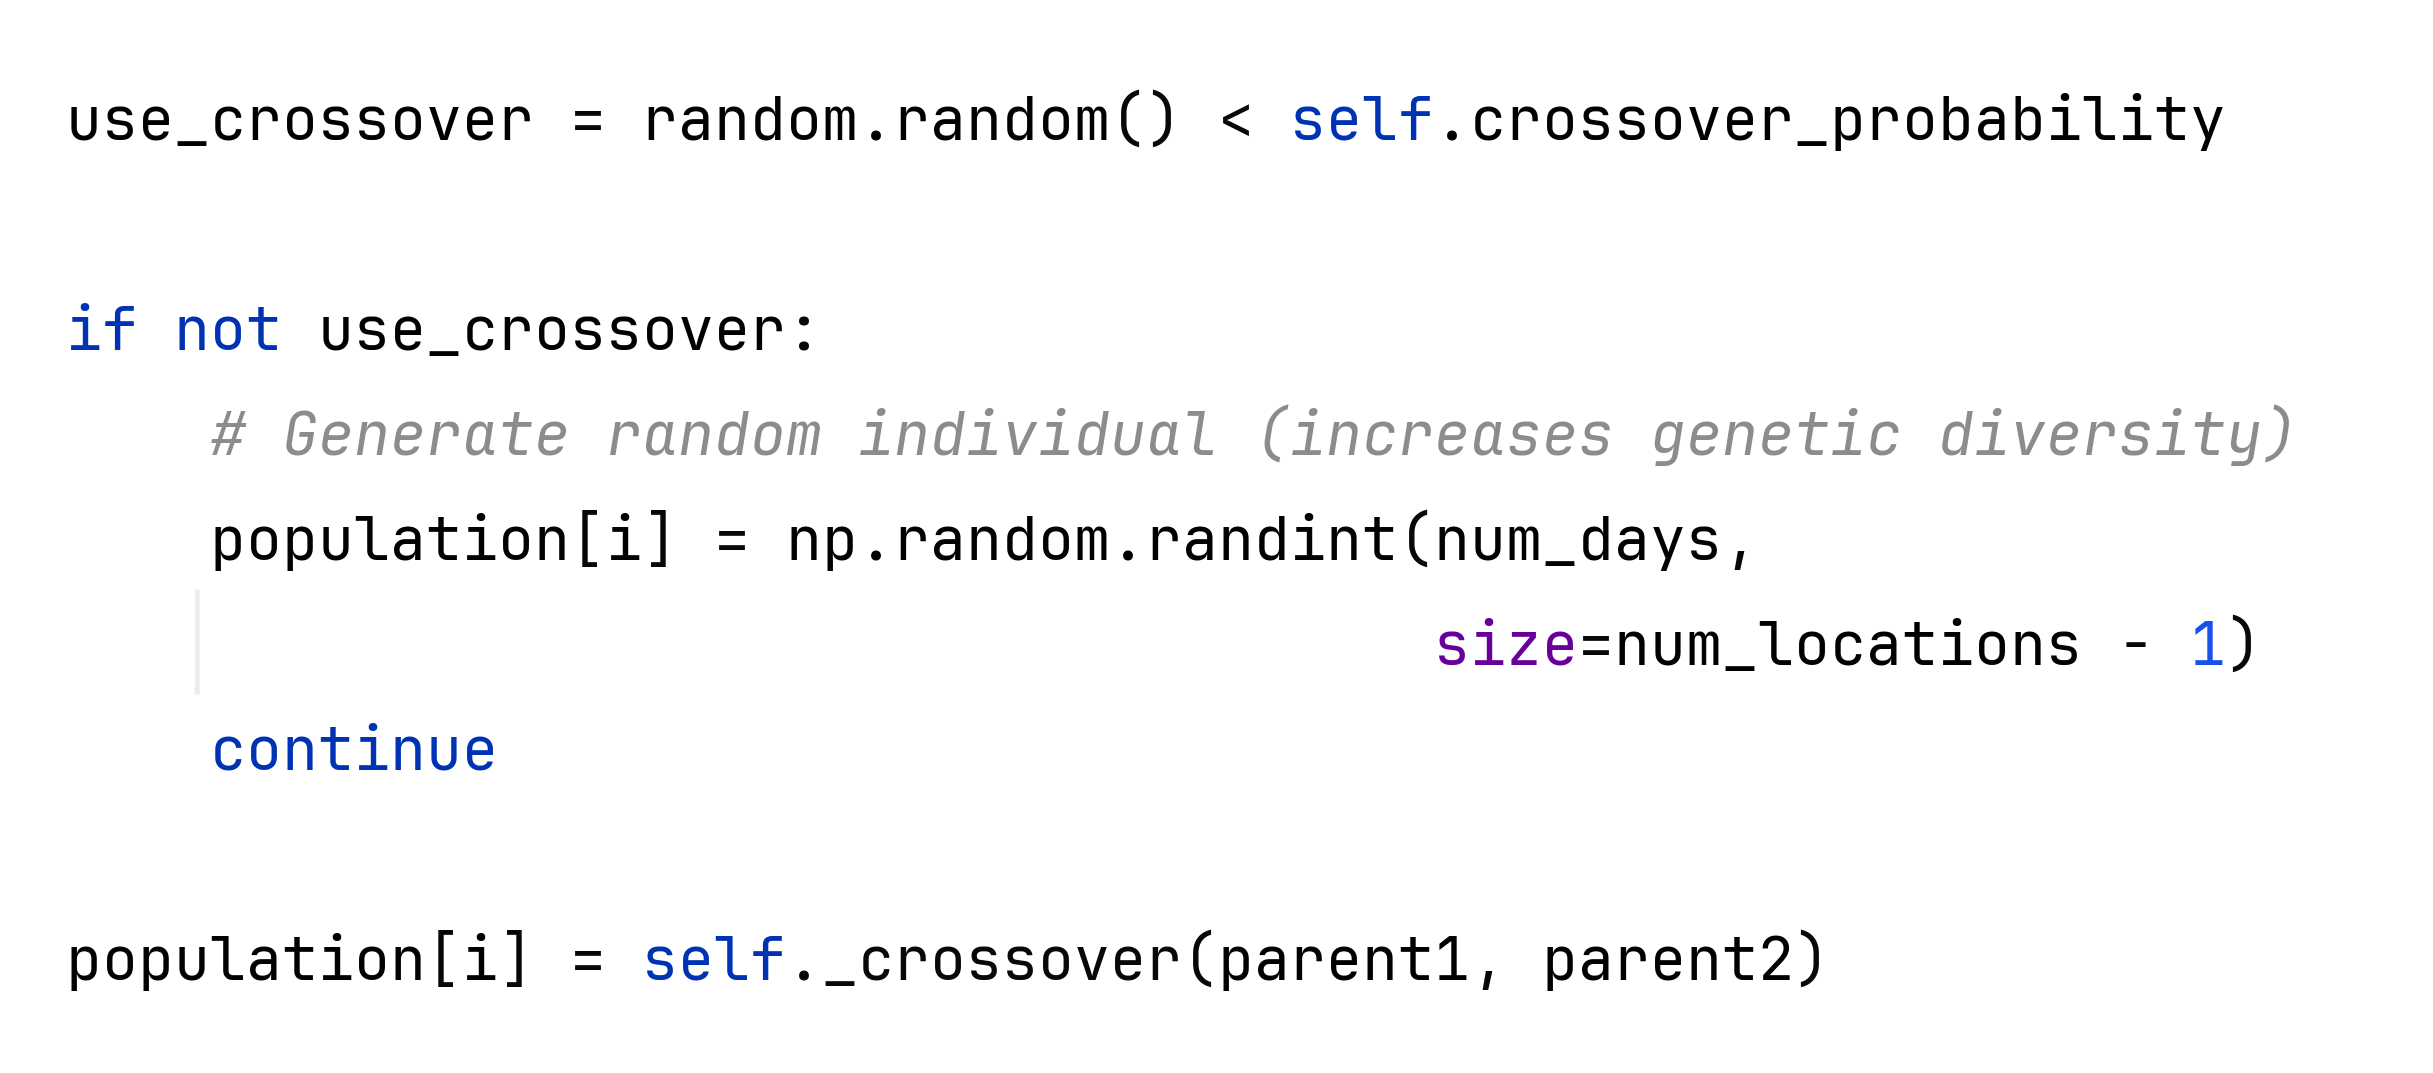
\includegraphics[width = \textwidth]{GeneticClustering.find_clusters.crossover}
    \caption{Code from GeneticClustering.find\_clusters in algorithms\textbackslash clustering.py}
    \label{fig:GeneticClustering.find_clusters.crossover}
\end{figure}

\noindent
For this implementation of crossover, a uniform crossover will be performed, using crossover masks.
A crossover mask is a bit array the same length as the genome, with the parity of each bit indicating which parent
to choose from for the corresponding bit in the created genome.
In a uniform crossover mask, each bit has an 50\% chance of being a 0 or 1, meaning that each bit in the offspring
genome has an equal chance of being from either parent~\parencite{syswerda1989uniform}.
If the two parents, being the best individuals in a population, agree on a bit it then it would appear likely to be a
good choice.
With this implementation of crossover, the offspring will always copy over the bits that parents agree on.
Figure~\ref{fig:Crossover_Mask_Example} shows an example of how a crossover mask can be used to create offspring from
two parents, the example uses a hypothetical input including 6 locations and 3 clusters.
\begin{figure}[H]
    \centering
    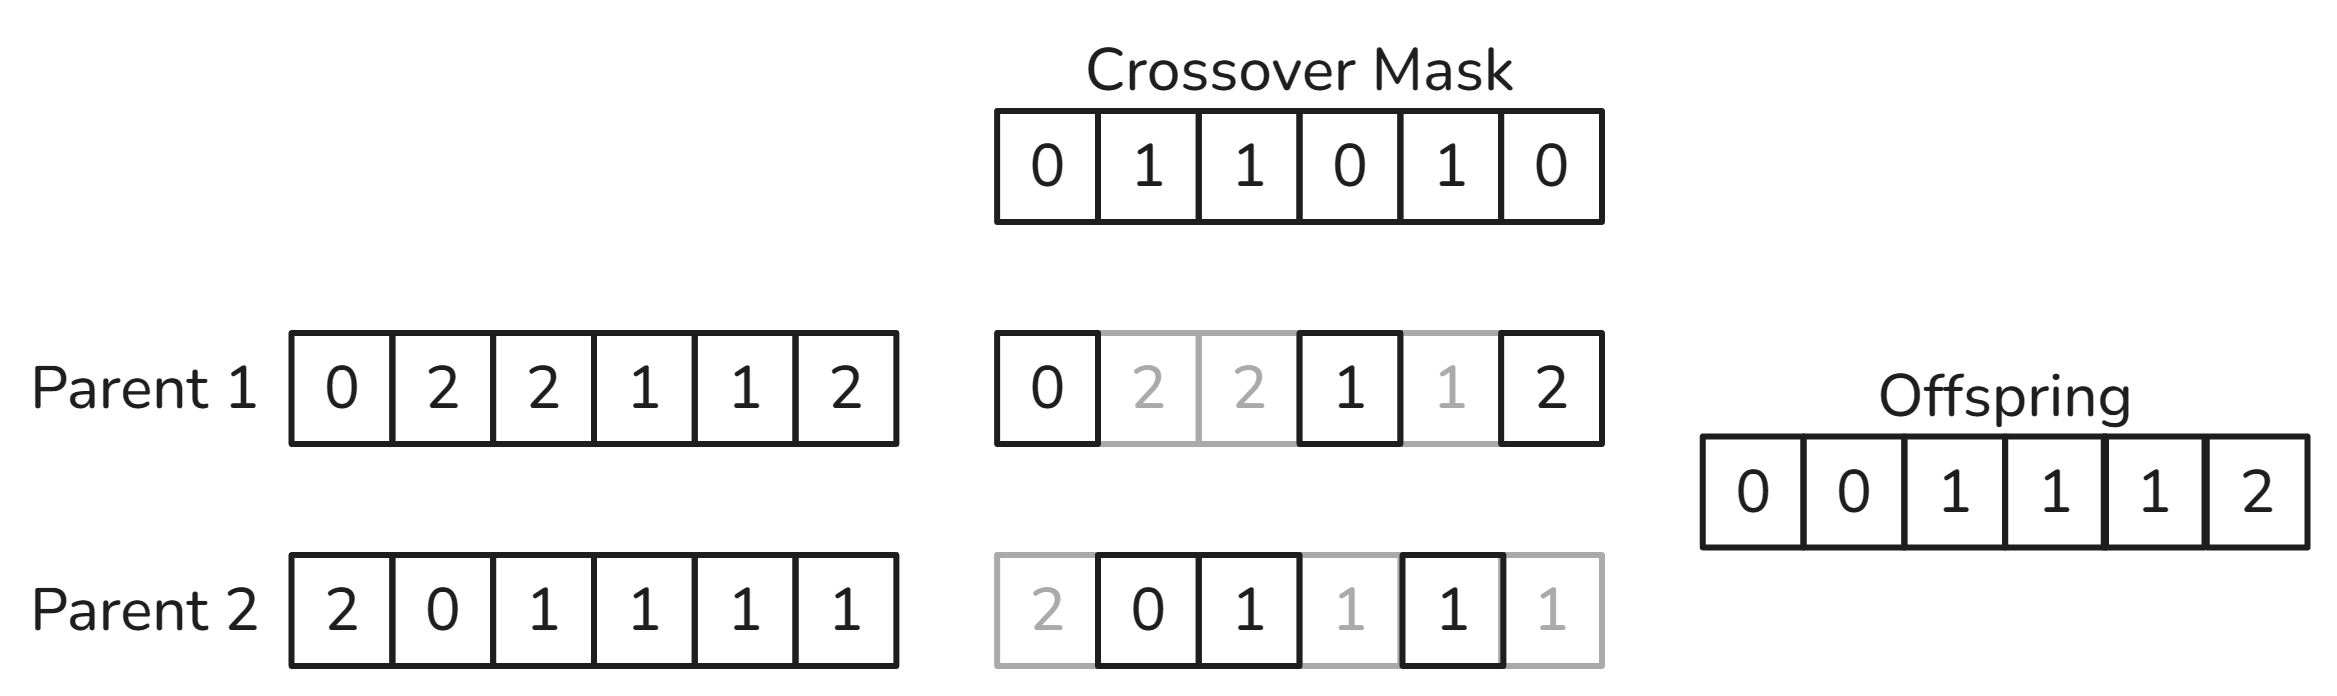
\includegraphics[width = \textwidth]{Crossover_Mask_Example}
    \caption{Example of using a crossover mask to create offspring from two parents.}
    \label{fig:Crossover_Mask_Example}
\end{figure}

\noindent
There is however, one slight issue with directly applying this method.
In the example shown in figure~\ref{fig:Crossover_Mask_Example}, parent 1's 0th cluster only includes the first
location, similarly, parent 2's 2nd cluster also only includes the first location.
Both parents are forming a cluster using these locations, however due to them being labelled differently, the
offspring produced did not continue this clustering.
To solve this problem a genome's clusters will be relabelled in order of their appearance in the genome, ensuring
consistency between parents.
Figure~\ref{fig:Crossover_Mask_Relabelling_Example} shows an example of this applied to the parents in figure~\ref{fig:Crossover_Mask_Example},
and figure~\ref{fig:GeneticClustering._relabel_individuals_clusters} shows how this is accomplished in python.
\begin{figure}[H]
    \centering
    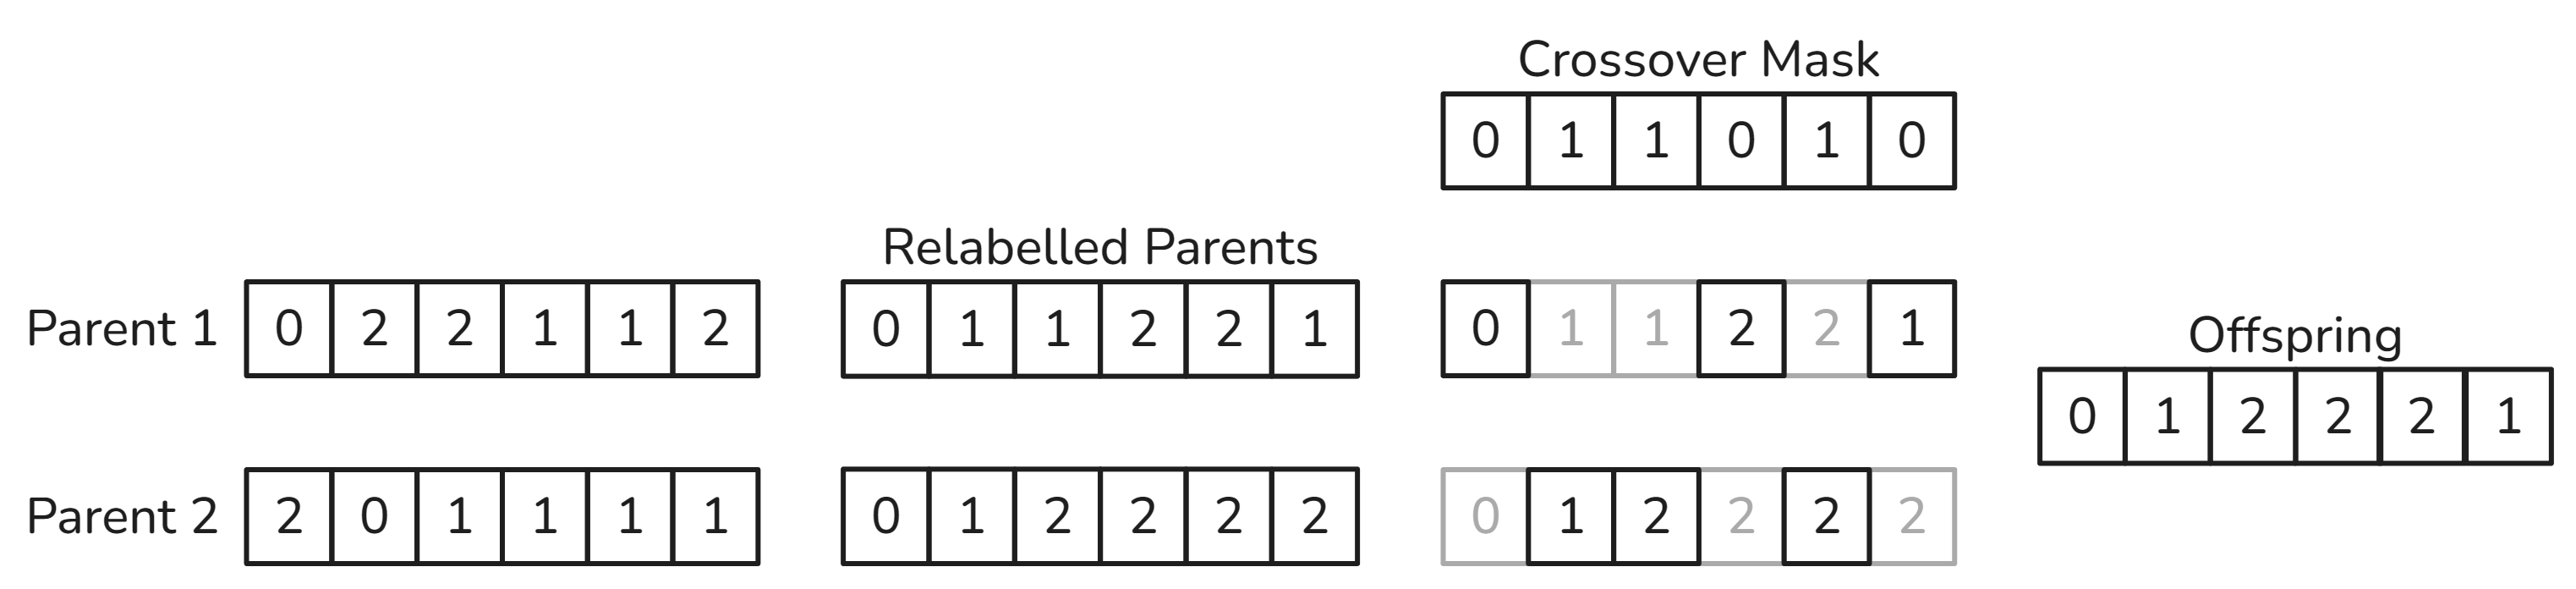
\includegraphics[width = \textwidth]{Crossover_Mask_Relabelling_Example}
    \caption{Example of relabelling a parent's clusters and the resultant offspring}
    \label{fig:Crossover_Mask_Relabelling_Example}
\end{figure}
\begin{figure}[H]
    \centering
    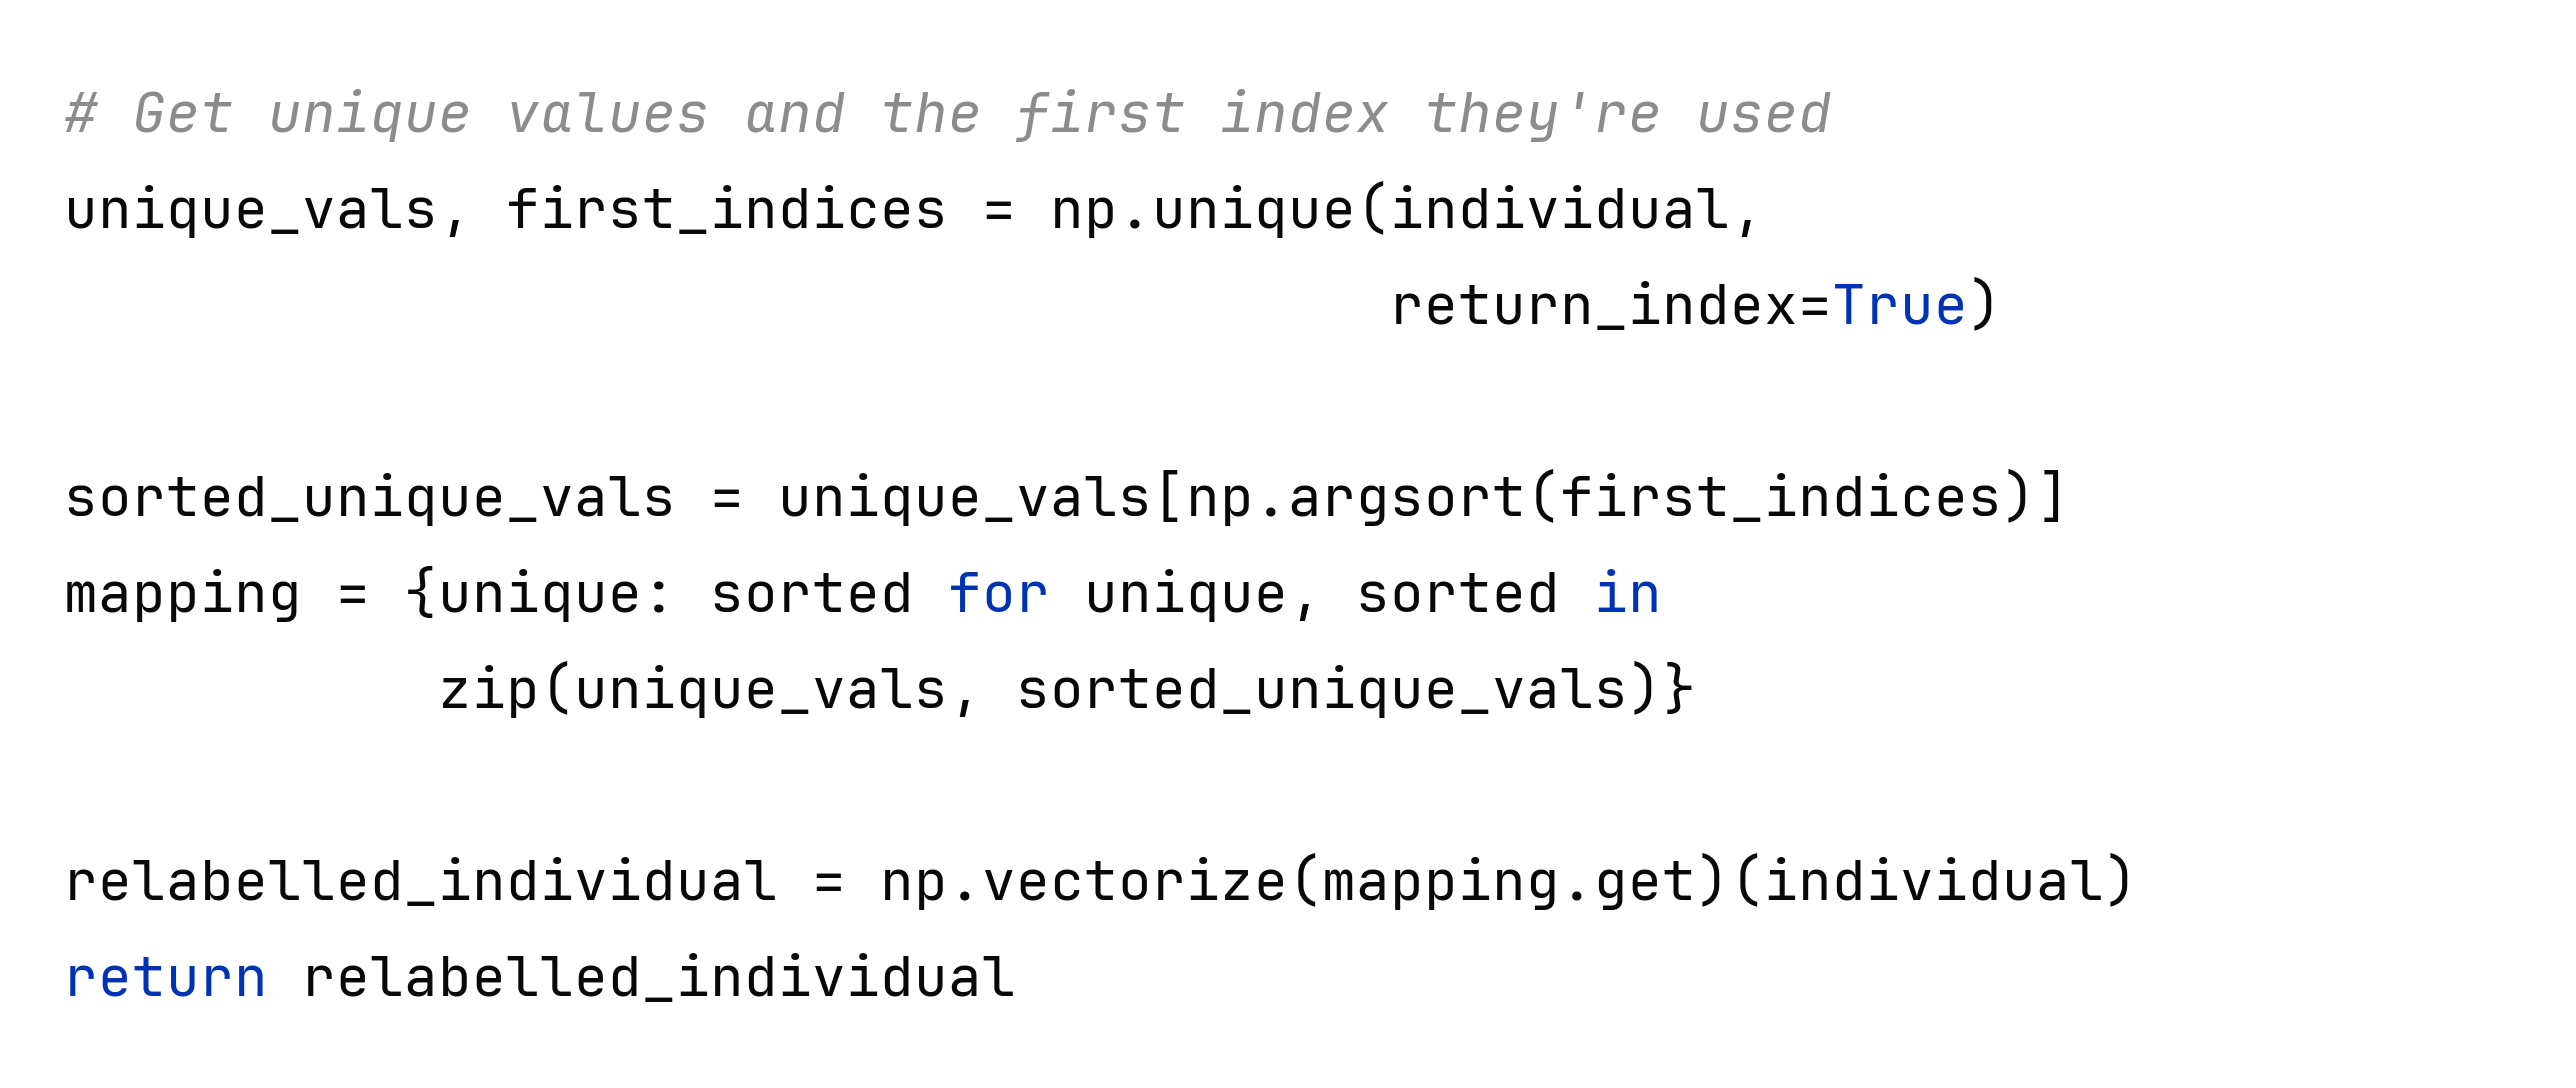
\includegraphics[width = \textwidth]{GeneticClustering._relabel_individuals_clusters}
    \caption{Code from GeneticClustering.\_relabel\_individuals\_clusters in algorithms\textbackslash clusterin.py}
    \label{fig:GeneticClustering._relabel_individuals_clusters}
\end{figure}

\noindent
After this relabelling, crossover can be performed without issue.
Figure~\ref{fig:GeneticClustering._crossover} shows the python implementation of this.
\begin{figure}[H]
    \centering
    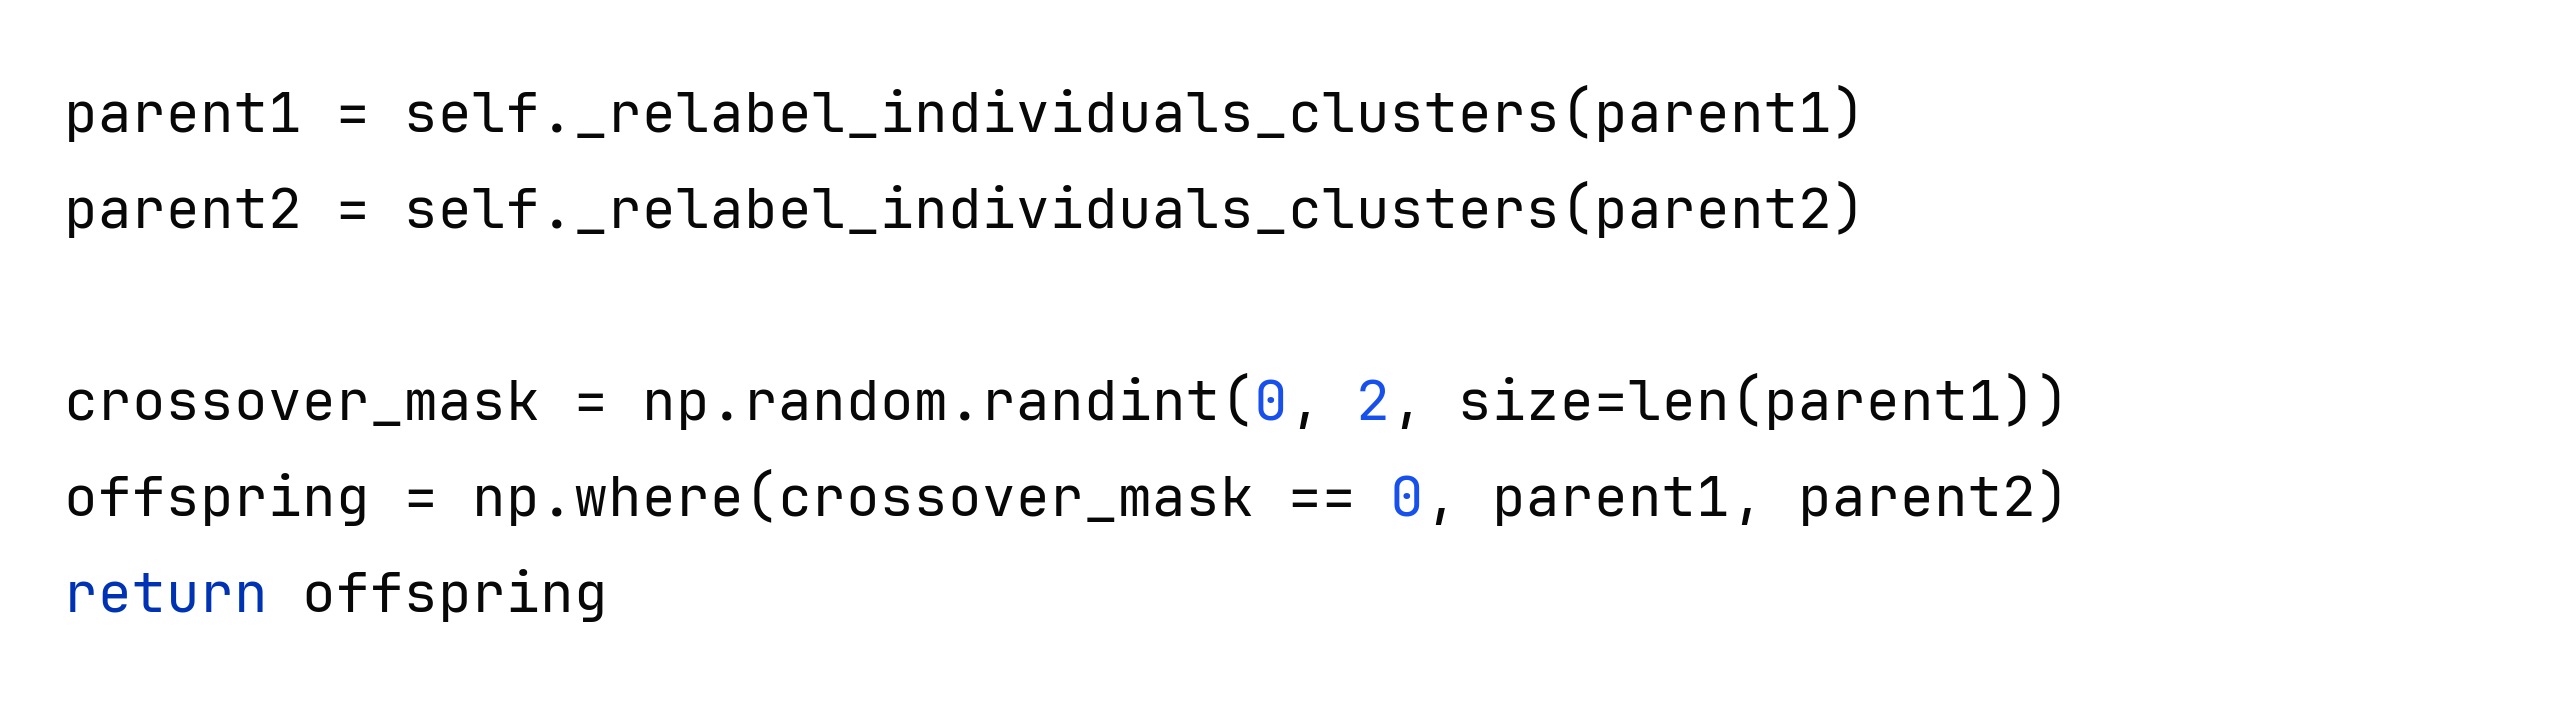
\includegraphics[width = \textwidth]{GeneticClustering._crossover}
    \caption{Code from GeneticClustering.\_crossover in algorithms\textbackslash clustering.py}
    \label{fig:GeneticClustering._crossover}
\end{figure}

After crossover is complete, created offspring are randomly mutated in the hopes of increasing genetic diversity
and escaping local optima.
The genome is mutated by iterating through each gene and randomly deciding if it will mutate or not, the likeliness
of mutation is decided by the mutation rate.
If a gene is chosen to mutate, it will assign itself to a random cluster.
Figure~\ref{fig:GeneticClustering.find_clusters.mutation} shows how this is implemented in python.
\begin{figure}[H]
    \centering
    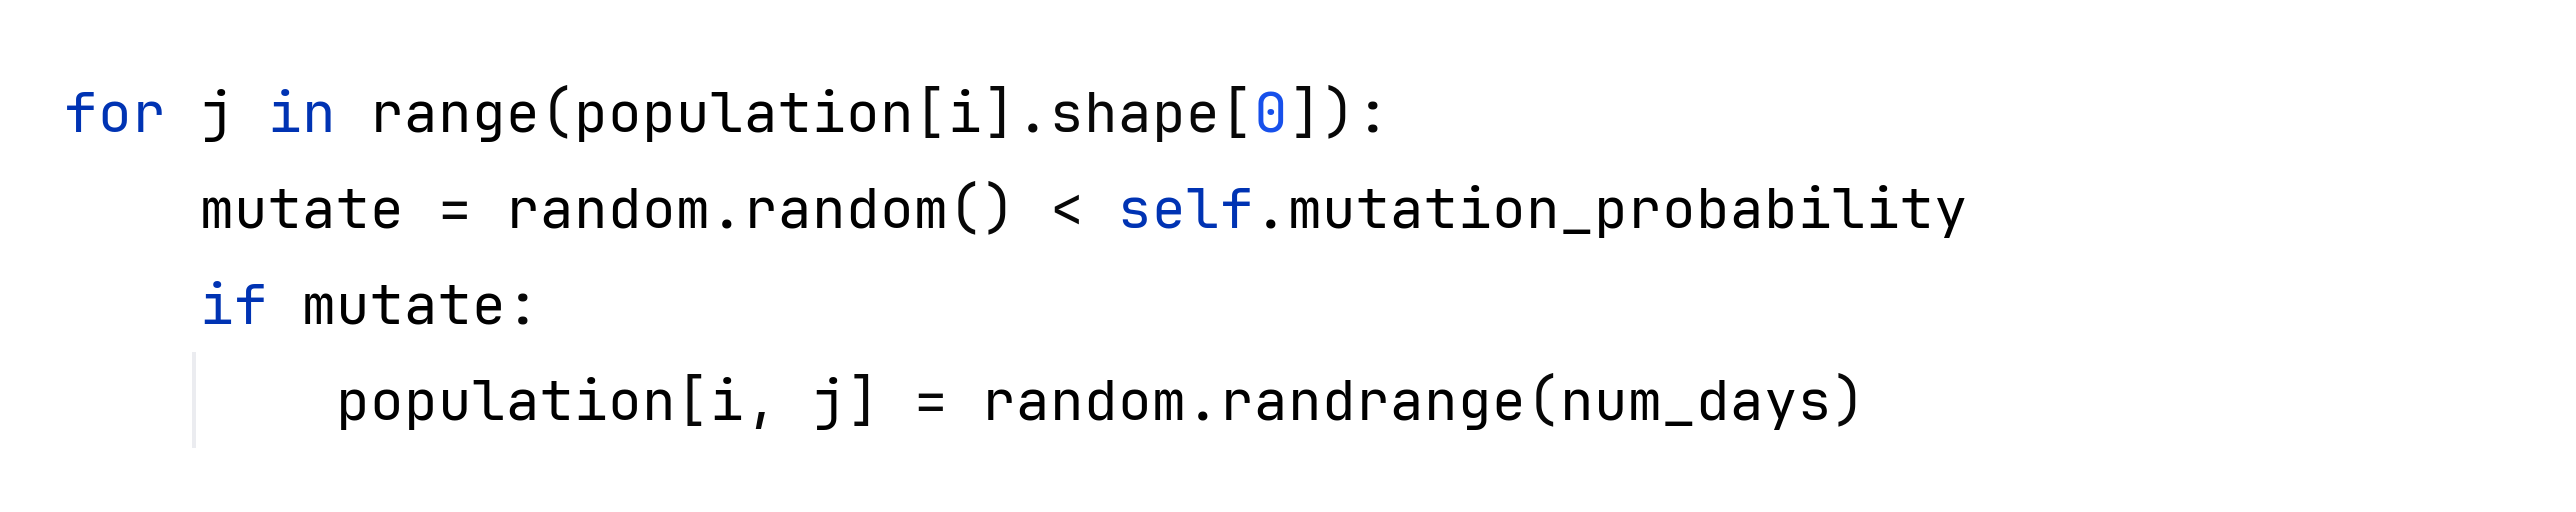
\includegraphics[width = \textwidth]{GeneticClustering.find_clusters.mutation}
    \caption{Code from GeneticClustering.find\_clusters in algorithms\textbackslash clustering.py}
    \label{fig:GeneticClustering.find_clusters.mutation}
\end{figure}

\noindent
After the new population has been created, the process is restarted for the next generation, repeating these steps
until a maximum number of generations is reached.
By time evolution is complete the population will hopefully have converged on a good solution.
Figure~\ref{fig:GeneticClustering_London_Generation1} shows an example of using Genetic Clustering the same input as
for the K-Means example in figure~\ref{fig:KMeans_London_Step1}.
In the example, Genetic Clustering is used alongside Greedy Routing (to be covered in section~\ref{subsubsec:greedy-routing})
to form a complete trip, the best routes found within their respective generations are shown.
Genetic Clustering was run for 30 generations with a population size of 12, a crossover rate of 0.9 was used
alongside a mutation rate of 0.1.
Figure~\ref{fig:GeneticClustering_London_Evaluations} shows a line graph of the best evaluation found for each
generation.
\begin{figure}[H]
    \ContinuedFloat*
    \centering
    \includegraphics[width = \textwidth]{GeneticClustering_London_Generation1}
    \caption{Genetic Clustering example, best route found in Generation 1.}
    \label{fig:GeneticClustering_London_Generation1}
\end{figure}
\begin{figure}[H]
    \ContinuedFloat
    \centering
    \includegraphics[width = \textwidth]{GeneticClustering_London_Generation5}
    \caption{Genetic Clustering example, best route found in Generation 5.}
    \label{fig:GeneticClustering_London_Generation2}
\end{figure}
\begin{figure}[H]
    \ContinuedFloat
    \centering
    \includegraphics[width = \textwidth]{GeneticClustering_London_Generation10}
    \caption{Genetic Clustering example, best route found in Generation 10.}
    \label{fig:GeneticClustering_London_Generation10}
\end{figure}
\begin{figure}[H]
    \ContinuedFloat
    \centering
    \includegraphics[width = \textwidth]{GeneticClustering_London_Generation30}
    \caption{Genetic Clustering example, best route found in Generation 30, evolution is now complete.}
    \label{fig:GeneticClustering_London_Generation30}
\end{figure}
\begin{figure}[H]
    \centering
    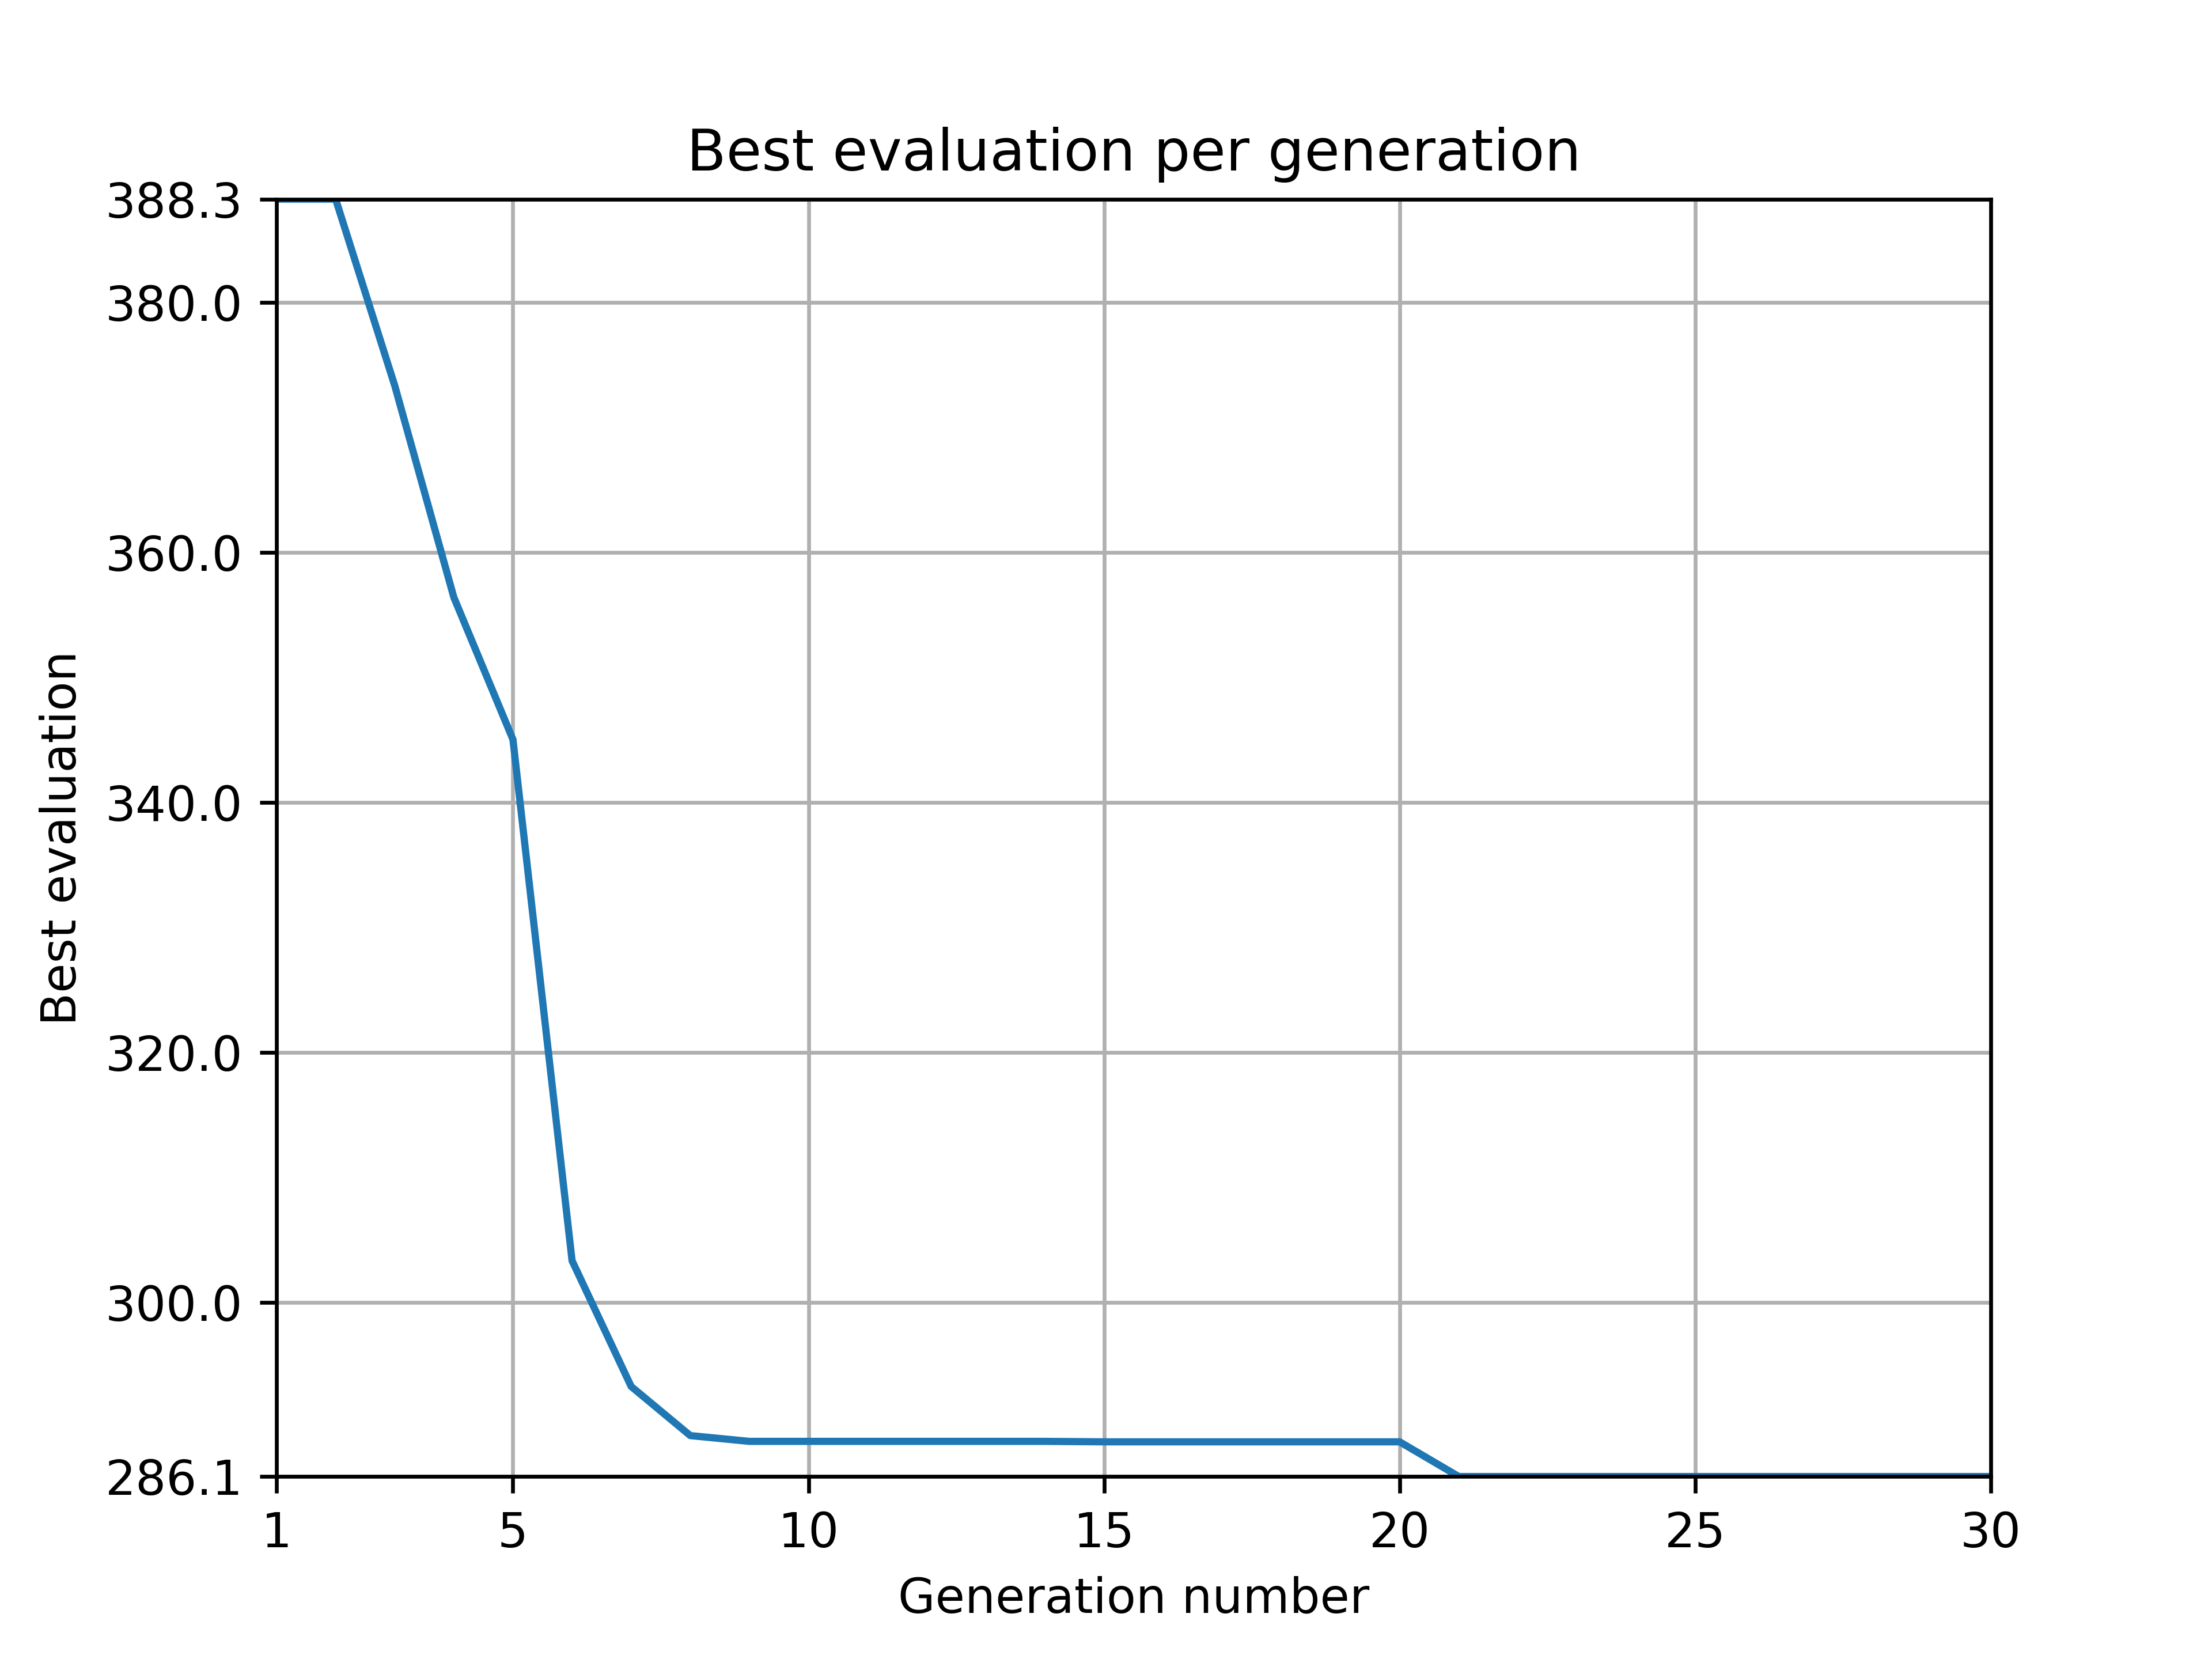
\includegraphics[width = \textwidth]{GeneticClustering_London_Evaluations}
    \caption{Line graph showing the best evaluation for each generation of clusters evolution process.}
    \label{fig:GeneticClustering_London_Evaluations}
\end{figure}

\noindent
Unlike K-Means, which finds optimal routes according to geographic base, Genetic Clustering is capable of optimising
across both optimisation objectives, finding short routes and minimising daily variance.
By evaluating each set of clusters according to the objective function, some assignment of locations to each day can be
found that will produce a good overall trip.
It is likely Genetic Clustering will run slower than traditional heuristic approaches such as K-Means, it will be of
interest whether the genetic approach can produce significantly better results as a trade off.

Genetic algorithms are also highly versatile and by modifying aspects of the algorithm can find solutions across a
number of problems.
This adaptability allows the implementation of genetic algorithms for route finding and trip generation approaches, as well
as performing a genetic centroid-based clustering similar to K-Means.
By comparing the performance of genetic algorithms against their counterparts across different approaches where they
perform best can be investigated.

\subsubsection{Centroid-Based Genetic Clustering}
Inspired by K-Means, Centroid-Based Genetic Clustering uses a genetic algorithm to find the best set of centroids
to cluster the data.
The same process of evolution is used, as described previously, except this time the genome will specify the
centroids to use for clustering.
With a different genome structure, the crossover and mutation methods will need be reconsidered.
Centroid Based Genetic Clustering keeps the same time complexity as Genetic Clustering, $O(g p r n)$, with $g$
being the number of generations, $p$ being the population size, $r$ being the time complexity of the chosen
routing algorithm and $n$ being number of locations and days.\\

\noindent
This genetic algorithms genome will be a list of coordinate pairs, representing the latitude and longitude of each
centroid.
Figure~\ref{fig:GeneticCentroids_Greenwich_Example} shows an example of how locations are clustered using a centroid-based genome.
\begin{figure}[H]
    \centering
    Genome: $\begin{bmatrix}0.00 & 0.01 & -0.01 & 0.00 & 0.00\\51.477 & 51.477 & 51.477 & 51.482 & 51.472\end{bmatrix}$
    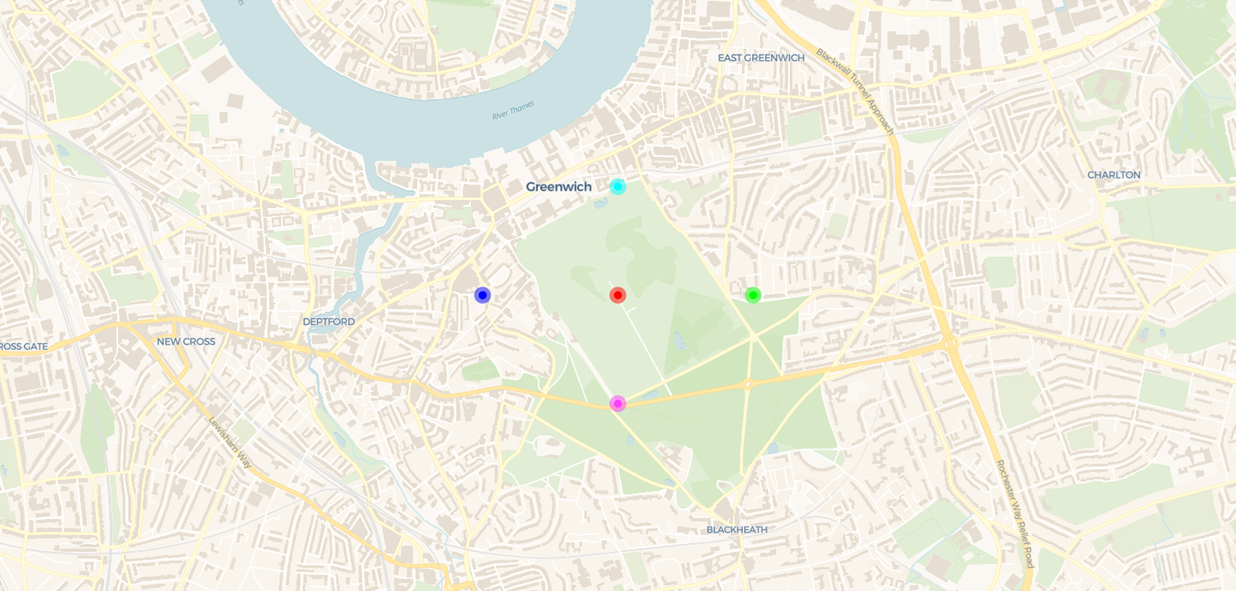
\includegraphics[width = \textwidth]{GeneticCentroids_Greenwich_Example}
    \caption{Example of how an individual's genome corresponds to cluster centroids.}
    \label{fig:GeneticCentroids_Greenwich_Example}
\end{figure}

\noindent
Once again, the population will be iteratively evolved through the process of selection, crossover and mutation.
The selection procedure here is largely the same in that each individual is evaluated by generating a trip with the help
of its genome and calculating the associated cost of these trips.
The only difference is that, because this genome is no longer a direct assignment of clusters, each location will first
need to be assigned to its nearest centroid.
This is shown in figure~\ref{fig:GeneticCentroids._evaluate_population}.
\begin{figure}[H]
    \centering
    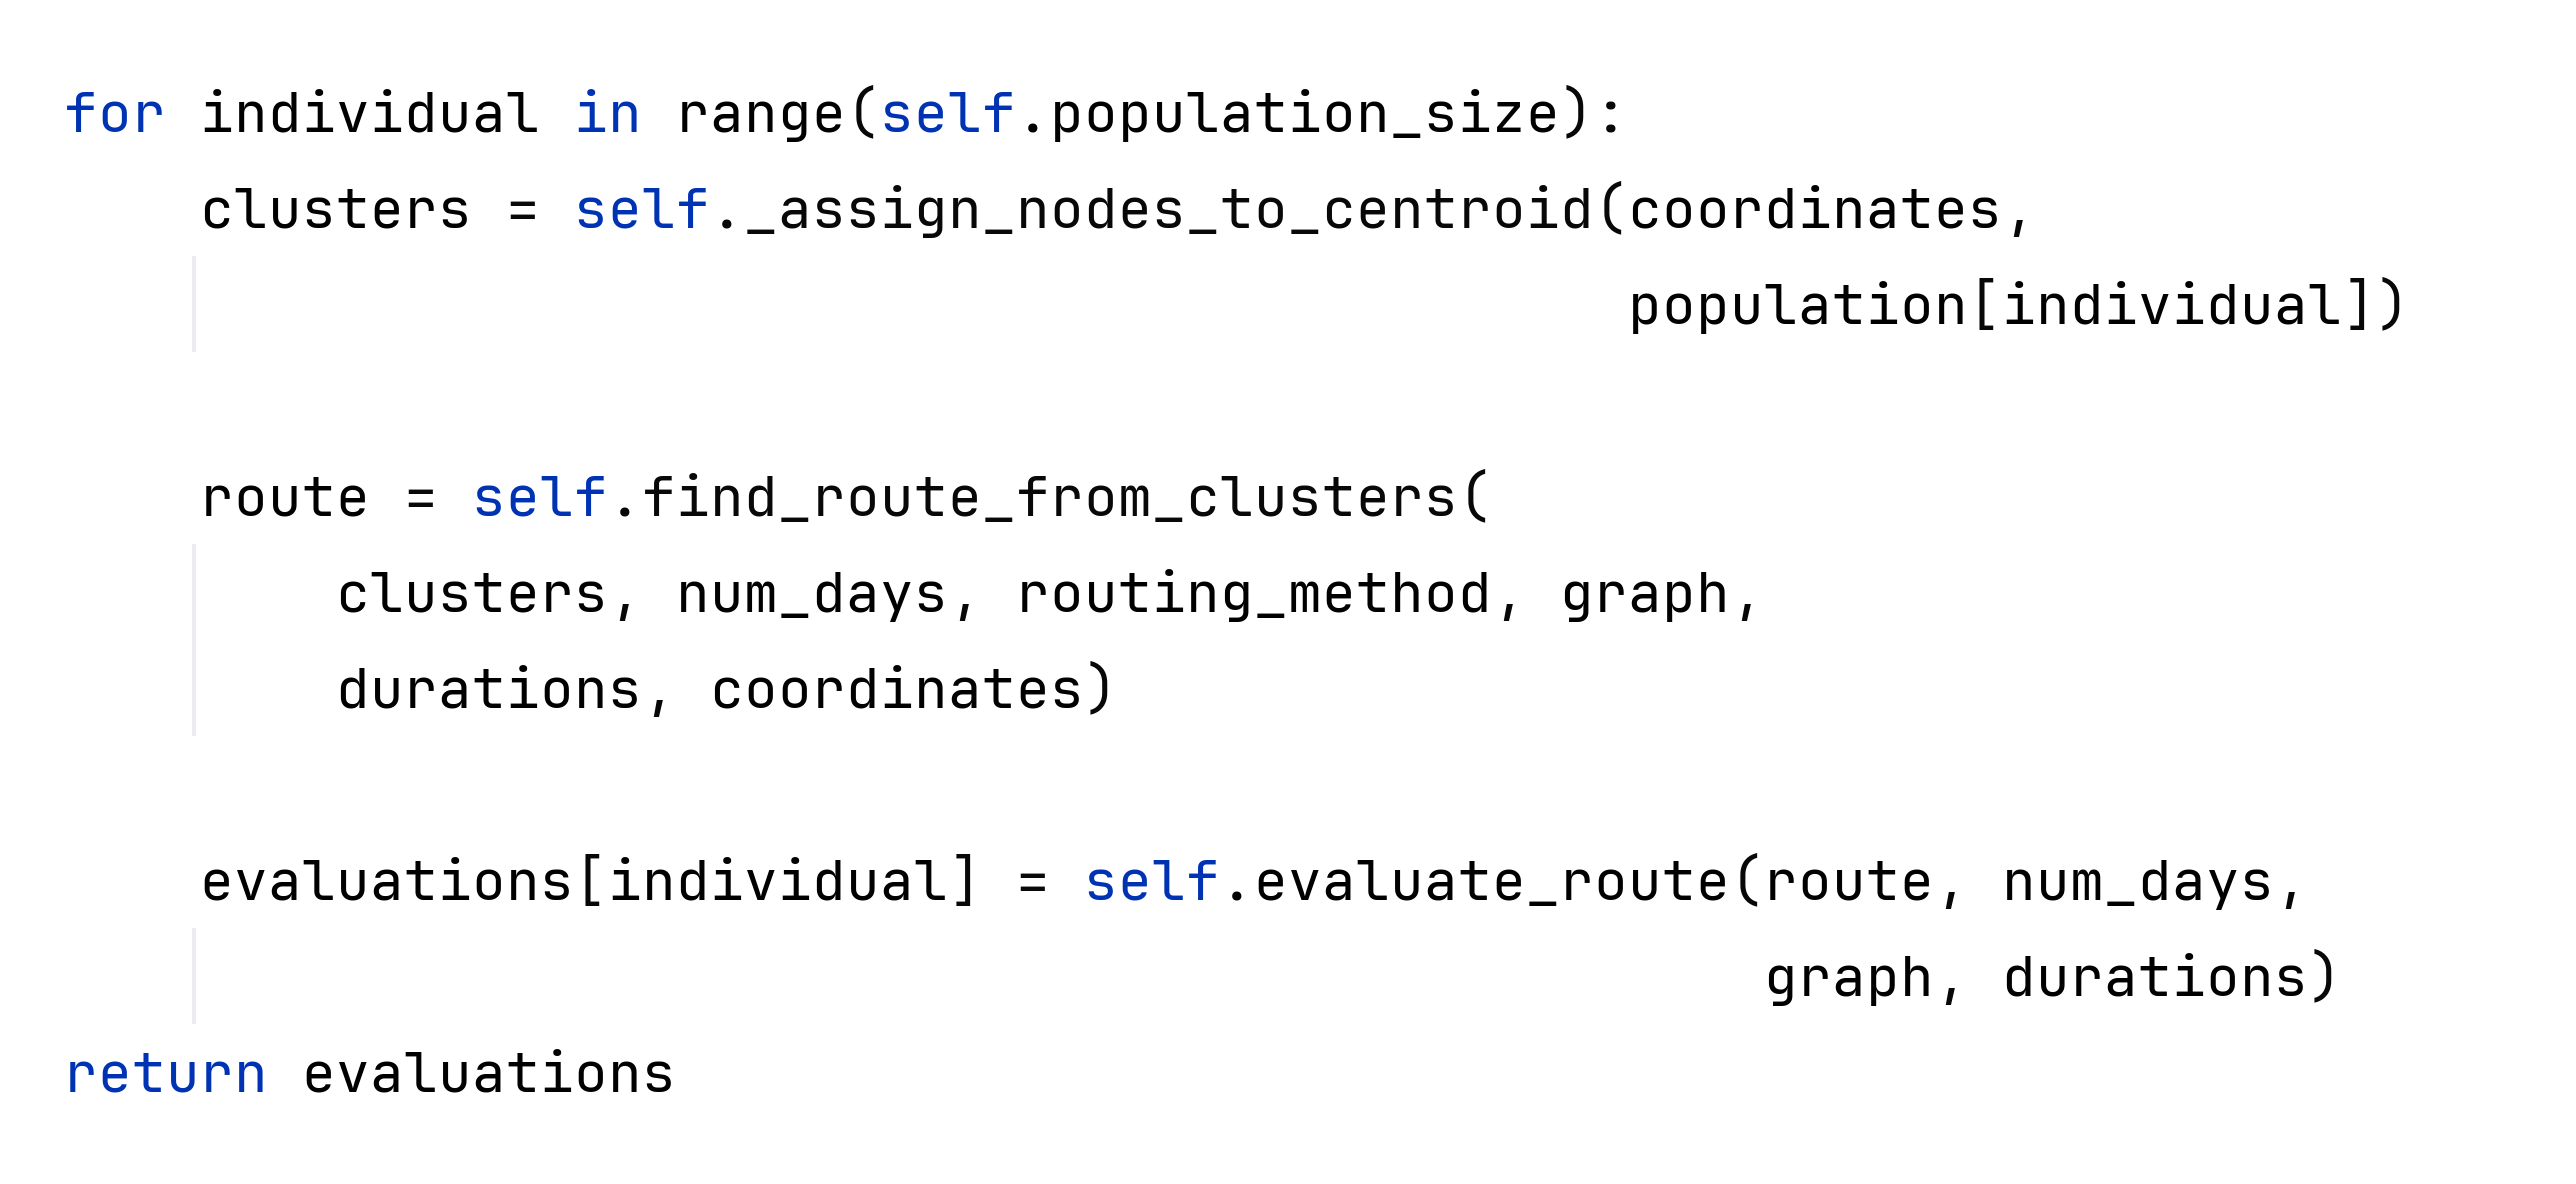
\includegraphics[width = \textwidth]{GeneticCentroids._evaluate_population}
    \caption{From GeneticCentroidClustering.\_evaluate\_population in algorithms\textbackslash clustering.py}
    \label{fig:GeneticCentroids._evaluate_population}
\end{figure}

\noindent
The `\_assign\_nodes\_to\_centroid' method shown in figure~\ref{fig:GeneticCentroids._evaluate_population} is the same
method used for K-Means, shown in figure~\ref{fig:Clustering._assign_nodes_to_centroid}.
With the population evaluated the best individuals can be selected for use in creating the next generation.
New generations are created via the same stages of copying over the best individuals, generating some new
individual's randomly and creating the rest via crossover and mutation.

For this implementation of crossover, instead of selecting random genes from each parent, the values of both parents
will be taken and merged together.
In practice, this means taking the coordinates of each centroid from both parents and finding a point between them
to generate a new centroid.
How close this new centroid is to each parent is determined by generating a random weight, indicating how much
influence each parent has on the offspring.\\

\noindent
Similarly to the previous implementation of crossover, the centroids will need to be reordered to ensure that both
parents are consistent with each other.
This time, because the genome isn't formed of discrete values that can be renamed, instead an approach of
finding the most similar centroids from each parent and merging them is taken.
This is performed by calculating the distances between each of parent 1's centroids to each of parent 2's, and
reordering the genome to place the closest centroids together.
Figure~\ref{fig:GeneticCentroids._crossover} shows this implementation of crossover, including how parents are
reordered and merged together to produce offspring.
\begin{figure}[H]
    \centering
    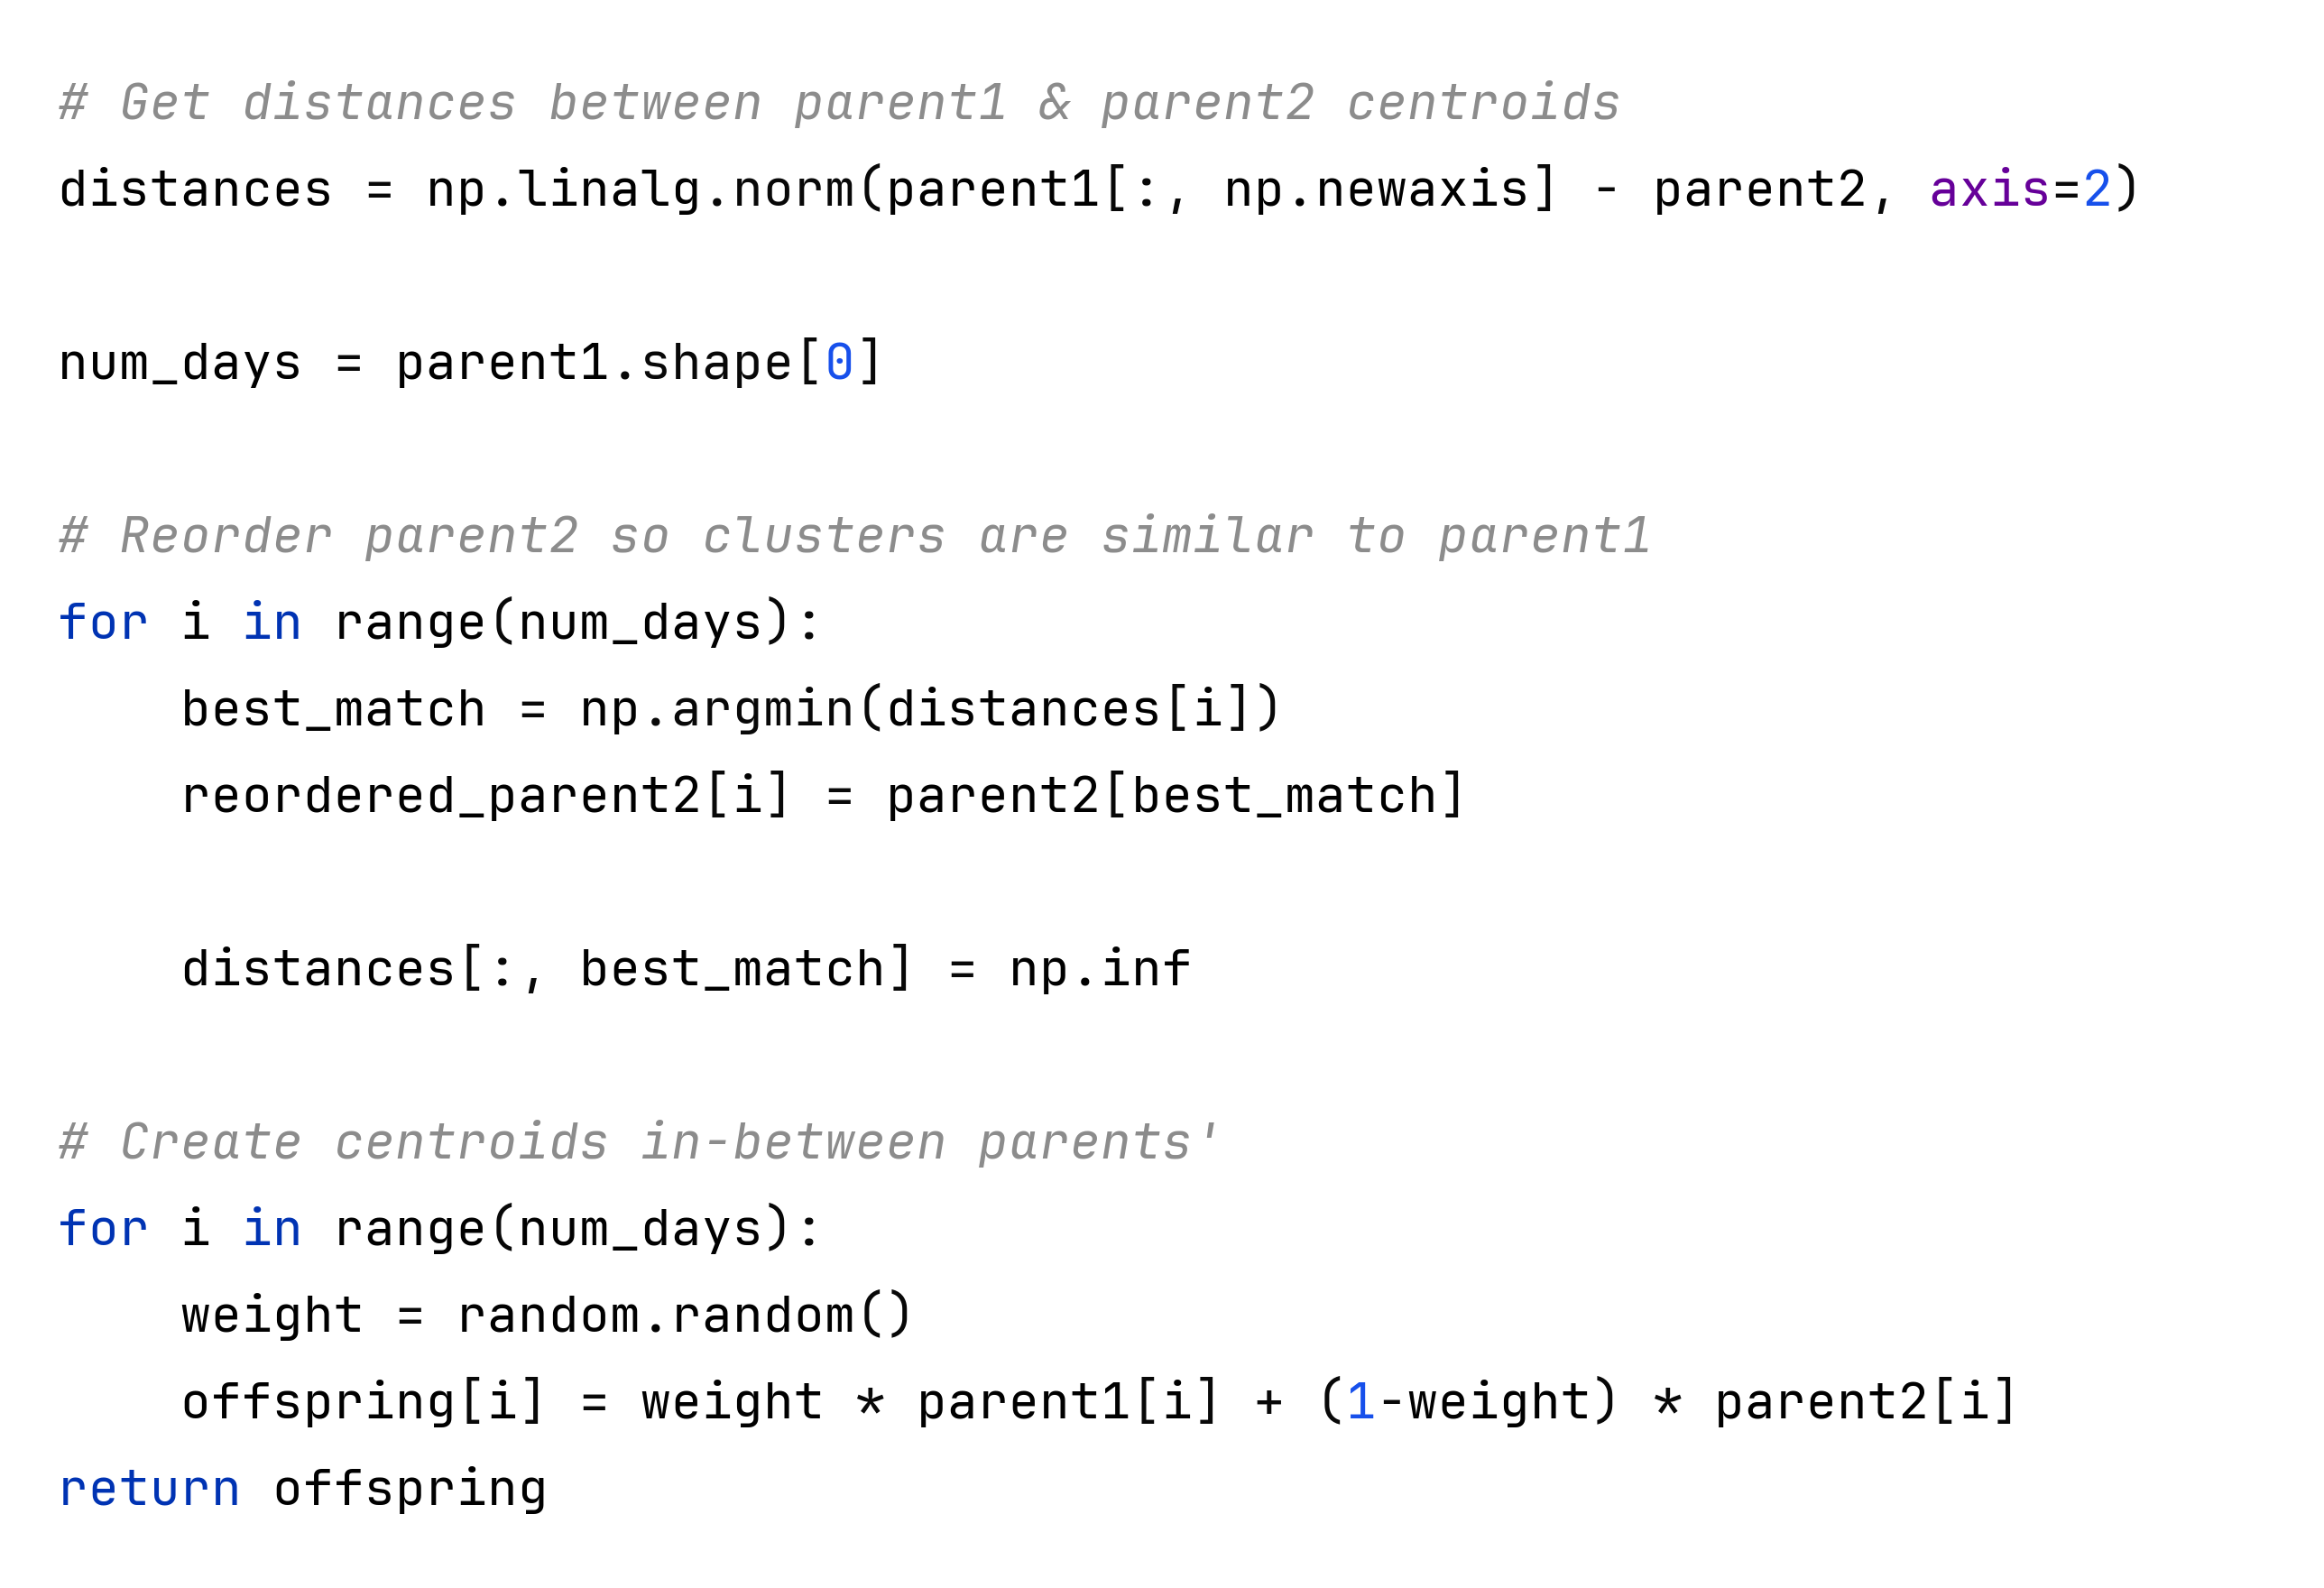
\includegraphics[width = \textwidth]{GeneticCentroids._crossover}
    \caption{Code from GeneticCentroidClustering.\_crossover in algorithms\textbackslash clustering.py}
    \label{fig:GeneticCentroids._crossover}
\end{figure}

\noindent
For mutation, each centroid of every individual will be considered, and a random decision taken as to whether the
centroid will mutate or not.
If a centroid is chosen to mutate, a new location will be within the bound of the input coordinates will be selected.
The minimum and maximum latitude and longitude of the input are used to form a region within which new centroids can
be generated, ensuring that the mutation is still relevant to the input.
Figure~\ref{fig:GeneticCentroids.find_clusters.mutation} shows this process of mutation.
\begin{figure}[H]
    \centering
    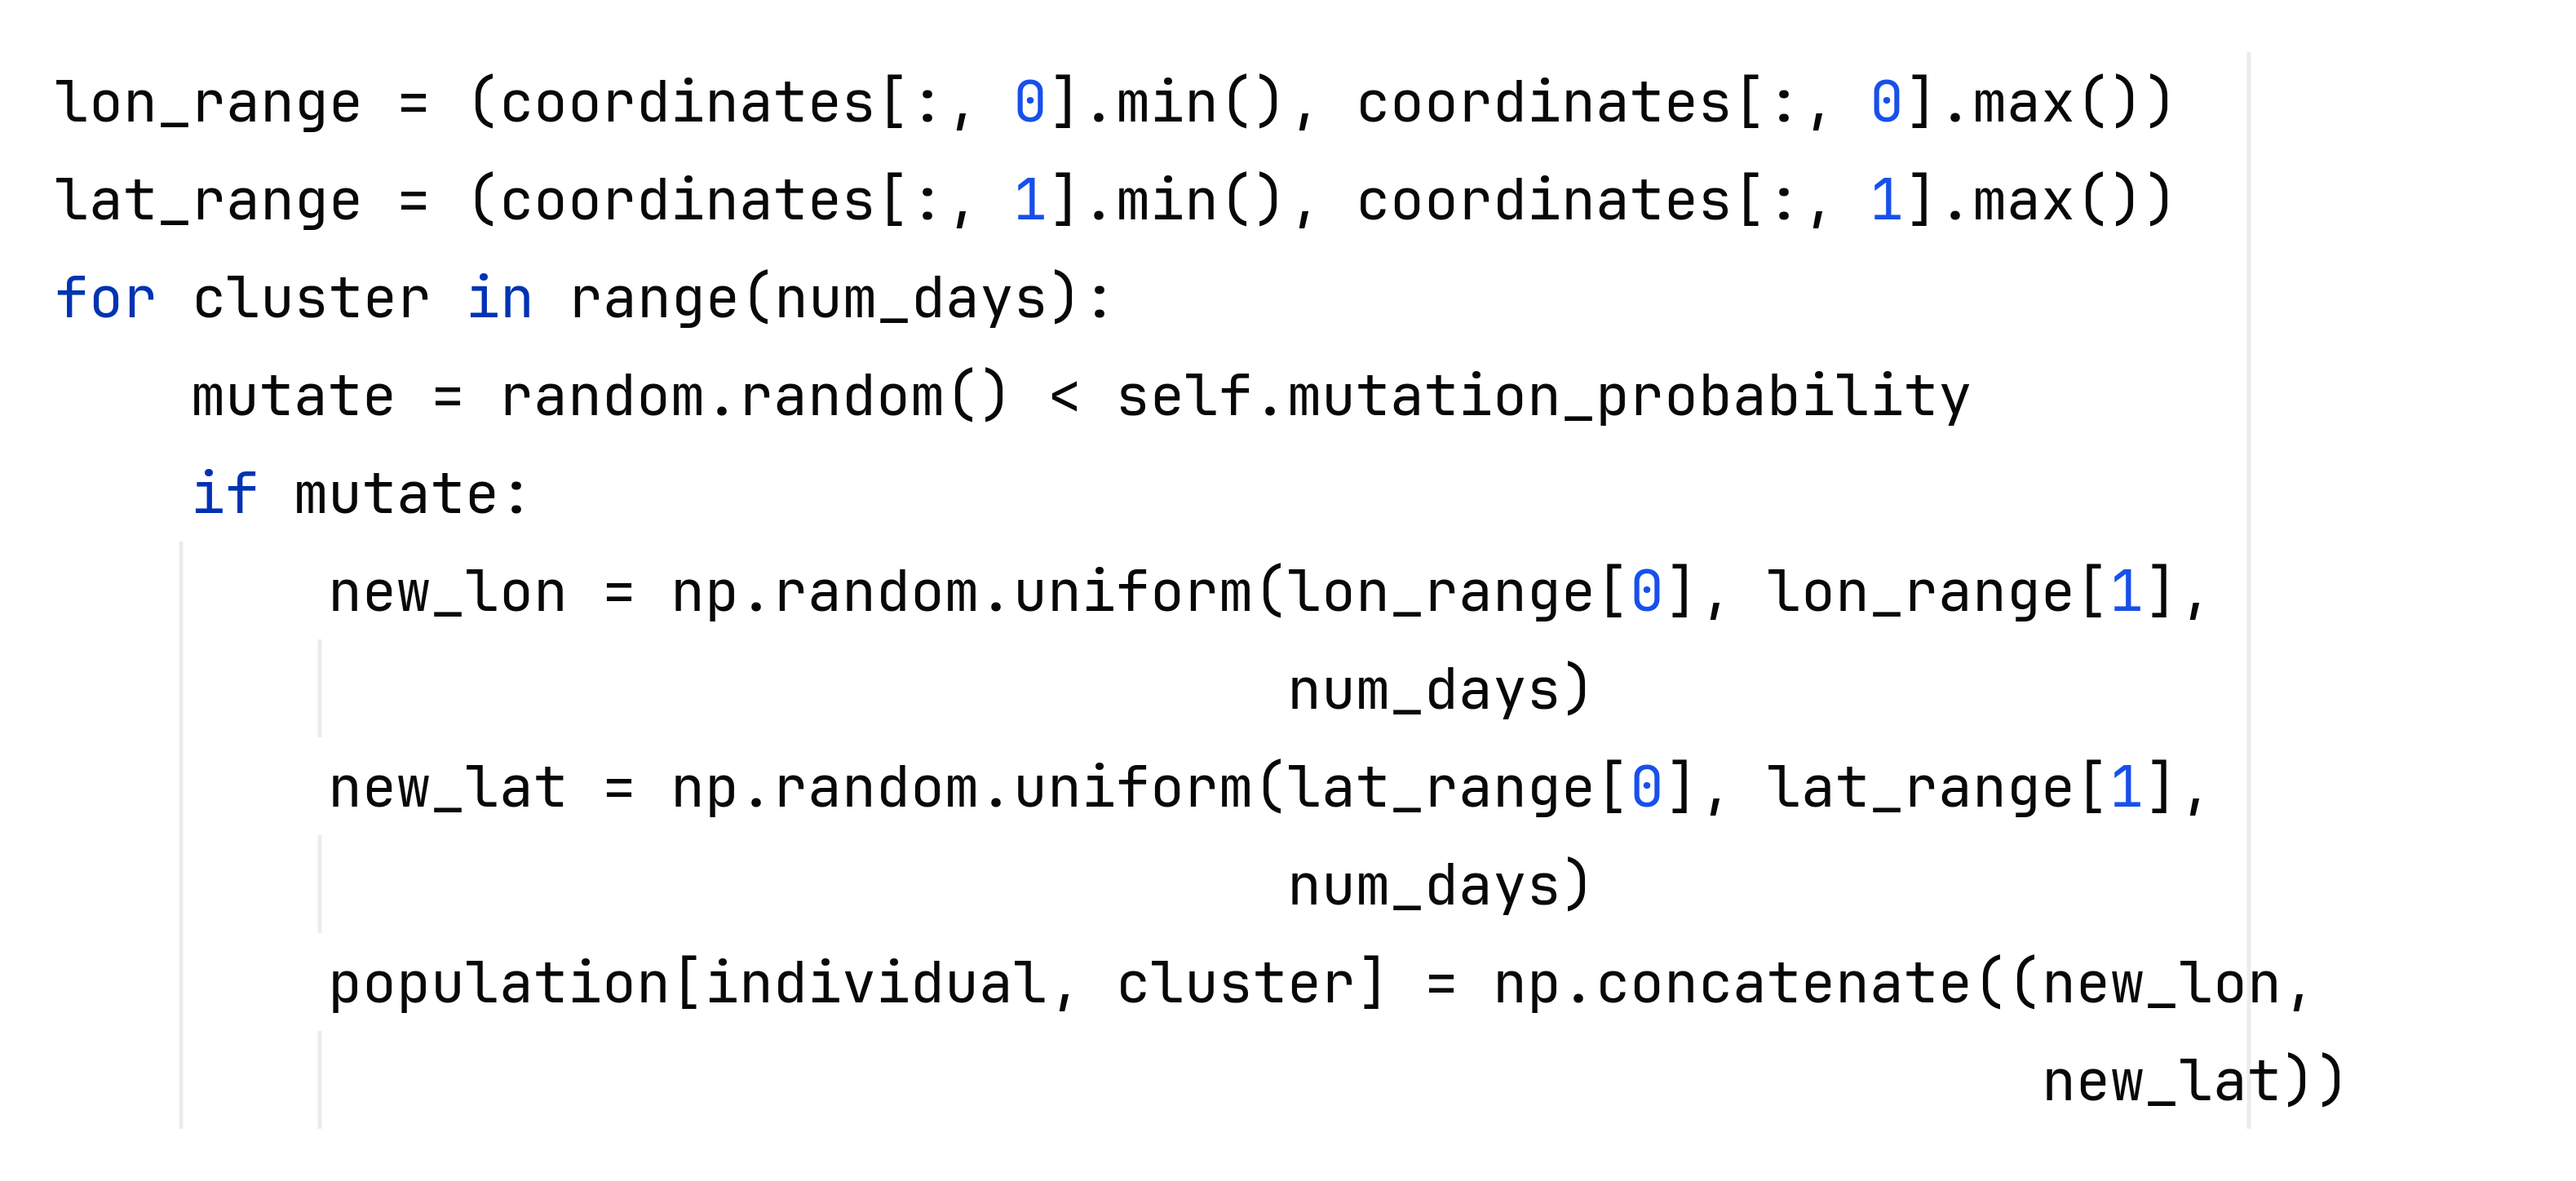
\includegraphics[width = \textwidth]{GeneticCentroids.find_clusters.mutation}
    \caption{Code from GeneticCentroidClustering.find\_clusters in algorithms\textbackslash clustering.py}
    \label{fig:GeneticCentroids.find_clusters.mutation}
\end{figure}

\noindent
Once again, this process of selection, crossover and mutation is repeated until a maximum number of generations is reached.
By the end of this process, a population of individuals that have been evolved to find good centroids for clustering the
input will have been identified.
Figure~\ref{fig:GeneticCentroids_London_Generation1} shows an example of genetic centroid-based clustering using the same
input as for previous clustering examples.
This example of genetic centroid-based clustering used the same hyperparameters as the previous genetic clustering
example, evolving 30 generations with a population size of 12, a crossover rate of 0.9, a mutation rate of 0.1 and
once again using Greedy Routing alongside found clusters to produce trips.
Again, a line graph of the best evaluation found for each generation of the process is shown in
figure~\ref{fig:GeneticCentroids_London_Evaluations}.
\begin{figure}[H]
    \ContinuedFloat*
    \centering
    \includegraphics[width = \textwidth]{GeneticCentroids_London_Generation1}
    \caption{Genetic Centroid Clustering example, best route found in Generation 1.}
    \label{fig:GeneticCentroids_London_Generation1}
\end{figure}
\begin{figure}[H]
    \ContinuedFloat
    \centering
    \includegraphics[width = \textwidth]{GeneticCentroids_London_Generation5}
    \caption{Genetic Centroids Clustering example, best route found in Generation 5.}
    \label{fig:GeneticCentroids_London_Generation5}
\end{figure}
\begin{figure}[H]
    \ContinuedFloat
    \centering
    \includegraphics[width = \textwidth]{GeneticCentroids_London_Generation10}
    \caption{Genetic Centroids Clustering example, best route found in Generation 10.}
    \label{fig:GeneticCentroids_London_Generation10}
\end{figure}
\begin{figure}[H]
    \ContinuedFloat
    \centering
    \includegraphics[width = \textwidth]{GeneticCentroids_London_Generation30}
    \caption{Genetic Centroids Clustering example, best route found in Generation 30, evolution is now complete.}
    \label{fig:GeneticCentroids_London_Generation30}
\end{figure}
\begin{figure}[H]
    \centering
    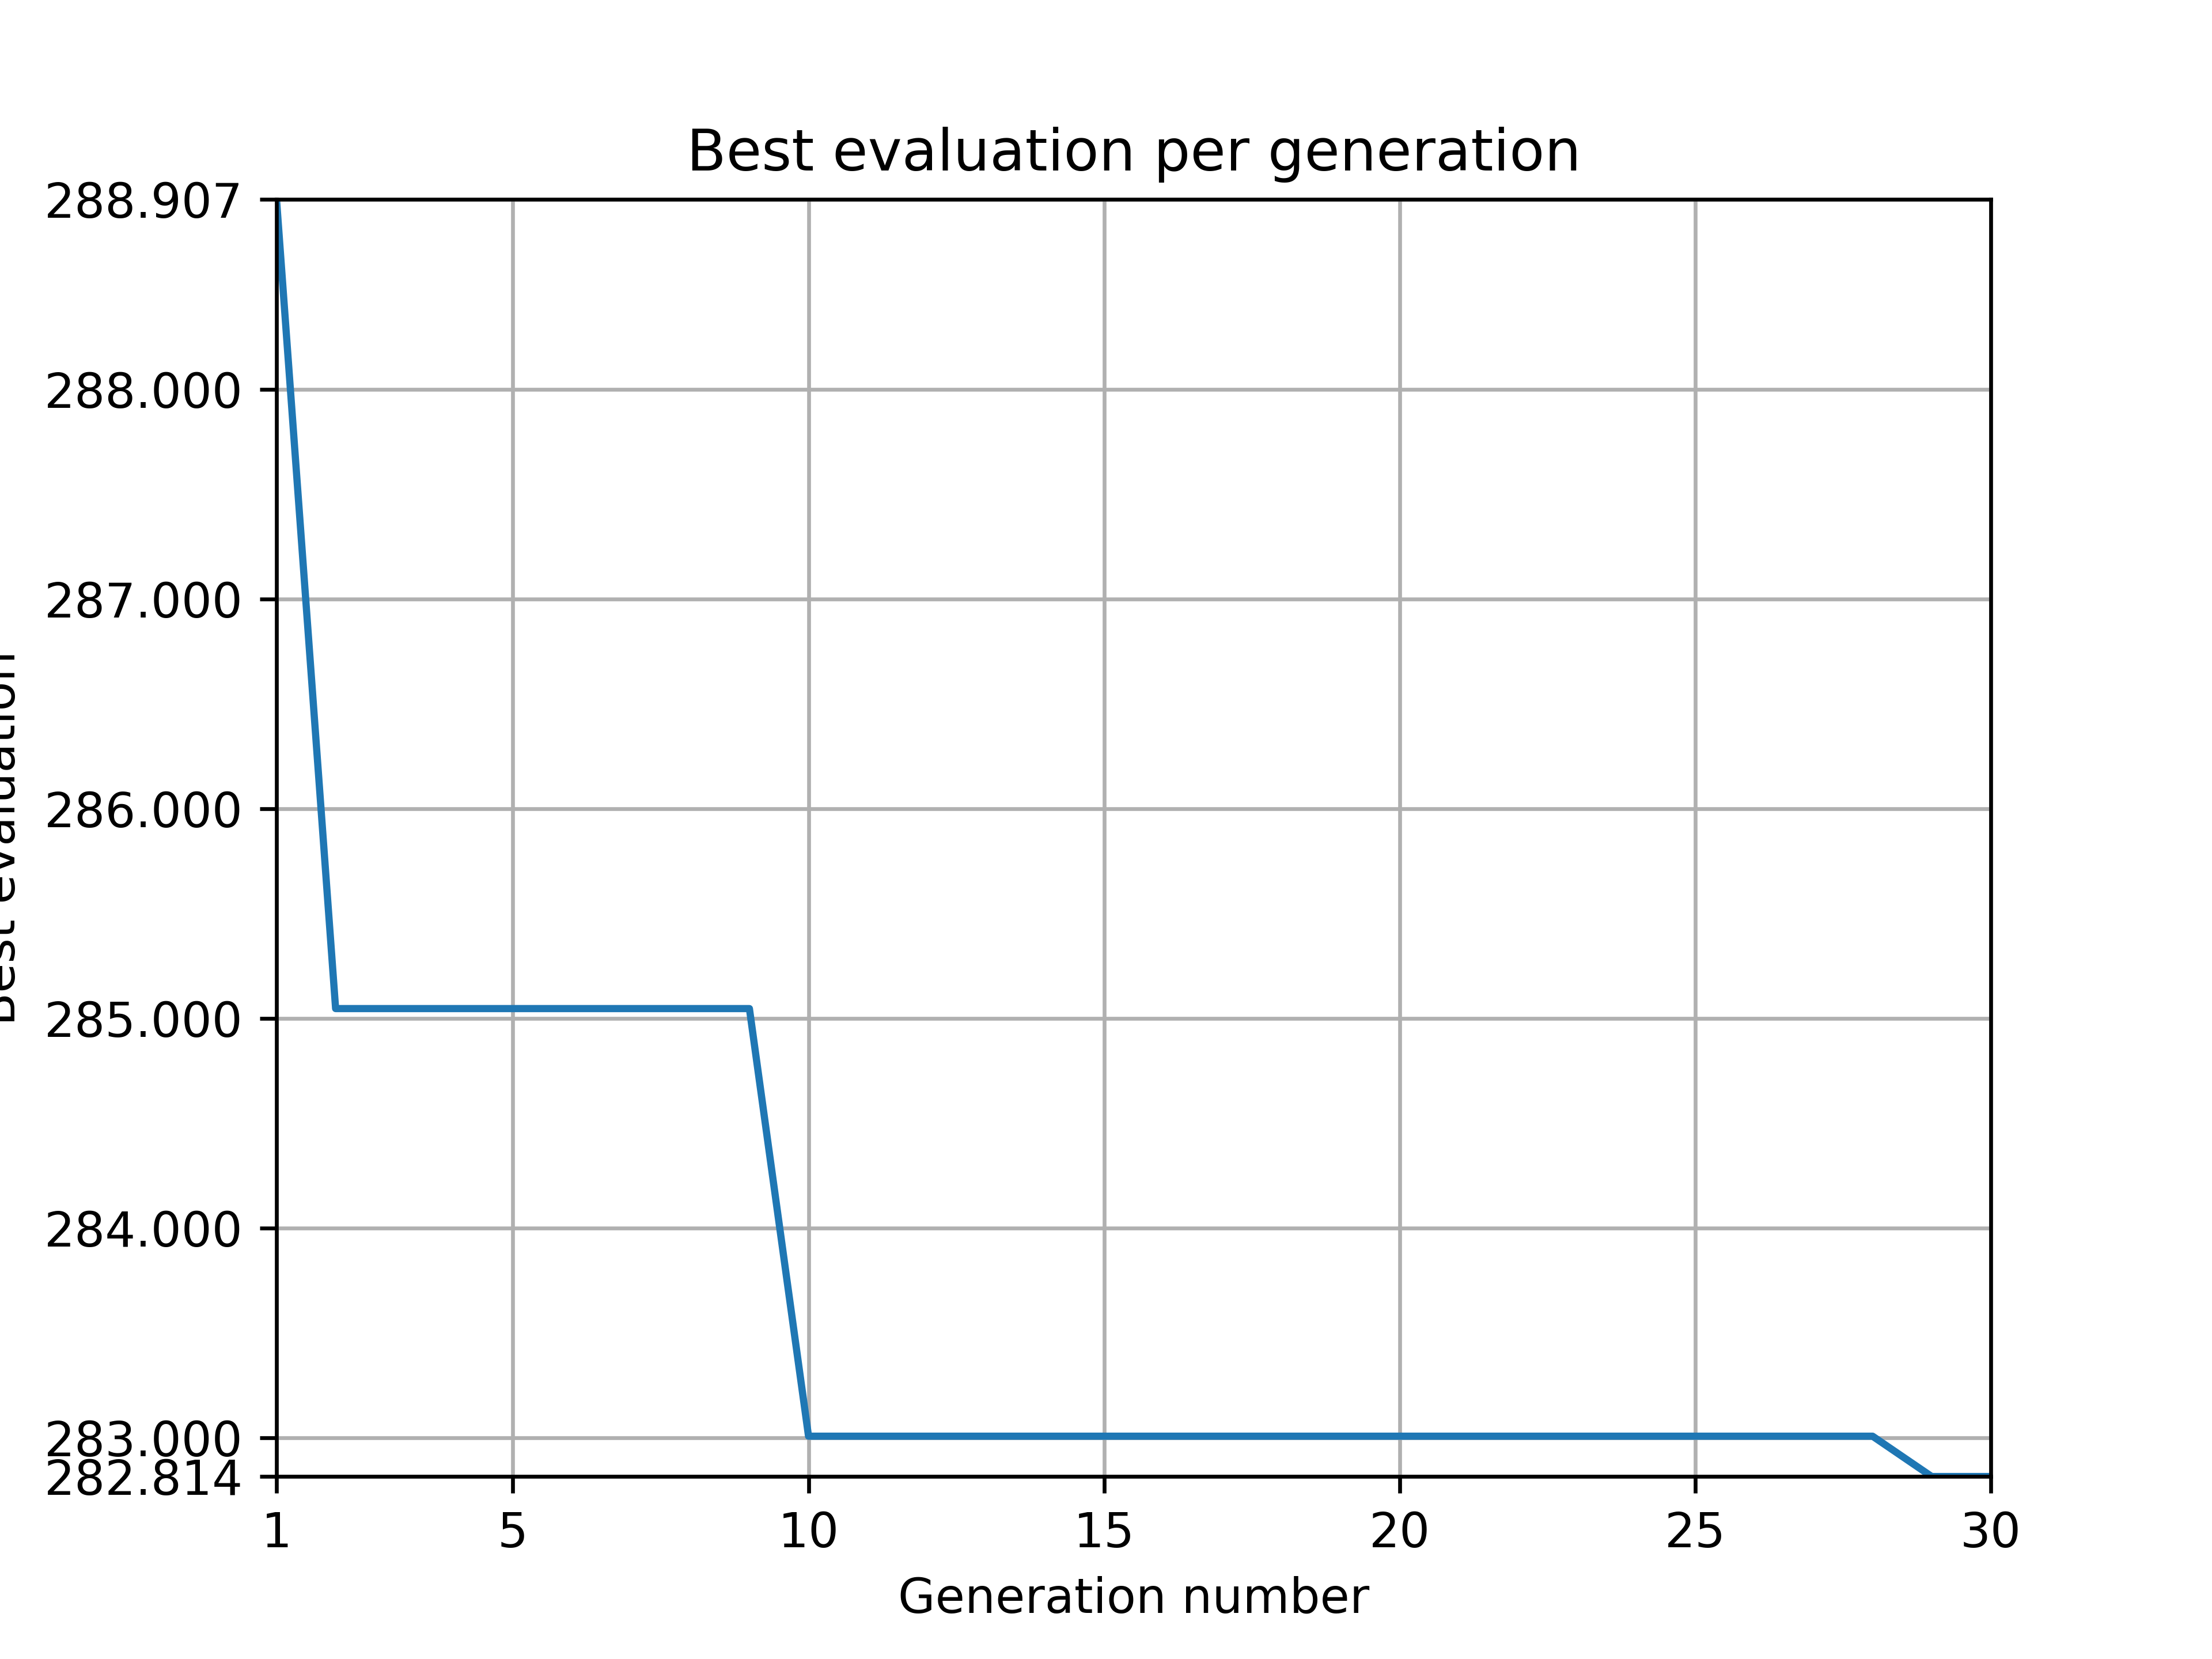
\includegraphics[width = \textwidth]{GeneticCentroids_London_Evaluations}
    \caption{Line graph showing the best evaluation for each generation of centroids evolution process.}
    \label{fig:GeneticCentroids_London_Evaluations}
\end{figure}
\noindent

\noindent
Genetic Centroid Clustering was included in this project to explore how a centroid-based approach, inspired by
K-Means, would perform when combined with a genetic algorithm.
Of particular interest is seeing how this approach compares to both standard K-Means as well as the other genetic
clustering approach.
Hopefully, by optimising chosen centroids according to the objective function, and exploring a wider range of potential
centroids, the quality of solution will be greater than that of regular K-Means.

\subsection{Routing}\label{subsec:routing}
The routing algorithms implemented in this project are TSP solvers, aiming to find a route with minimal travel time
that visits all given locations.
There are two ways in which routing will be used to form a trip either by using a clustering algorithm and then
finding a route for each cluster (as previously described in section~\ref{subsec:clustering}), or by finding a route
that visits every location, before splitting the route into multiple days.
This approach of splitting a route into multiple days will be covered Greedy Insertion is introduced.
algorithm which, on top of finding routes of its own, can also be used to build upon existing routes.
The routing algorithms implemented in this project are: Brute Force Routing, Greedy Routing, Greedy Insertion, Convex
Hull-Based Routing and Genetic Routing.

\subsubsection{Brute Force Routing}\label{subsubsec:brute-force-routing}
Brute Force Routing is an exhaustive algorithm that tries every possible route to find one with the least cost.
We find every route by generating all permutations of the locations to be visited, with the order of the locations
in each permutation representing the order in which they will be visited.
Each permutation is evaluated based on the amount of time it takes to travel the route, with the shortest route being
returned.
By checking every route Brute Force is guaranteed to find the best possible route, but due to checking every permutation
has a time complexity of $O(n!)$, where $n$ is the number of locations.

\noindent
It is worth noting that in this implementation, since all routes must return to the starting point, the final location
of a route is fixed.
Therefore, only $n-1$ locations need considering, resulting in $(n-1)!$ possible permutations.
To check every route, we'll be creating a mapping between every integer $\{0, 1, \mathellipsis, (n-1!)-1\}$ to every
permutation.
For a given integer $k$, and a list of possible locations $L: \{0, 1, \mathellipsis, n-1\}$ $k$'s corresponding
permutation can be obtained through the following steps:
\begin{enumerate}
    \item Divide $k$ by $(n-2)$ to find $x_1: \{0\leq x<n-1\}$, and the remainder $r_1$.
    \item $x_1$ is used to select a location for $L$, which will be the first location in the permutation. $L_{x_1}$ is
    removed from L.
    \item Divide $r_1$ by $(n-3)!$ to find $x_2: \{0\leq x<n-2\}$, and the remainder $r_2$.
    \item $x_2$ is used to select another location from $L$, which will be the second location in the permutation.
    Again, $L_{x_2}$ is removed from L.
    \item Repeat this process until all locations are assigned a position.
\end{enumerate}

\noindent
To help explain this, an example is shown in figure~\ref{fig:permutation-calculation-example}, generating a
permutation $P$ of the set $L = \{a, b, c, d\}$ that maps to $k = 17$.
\begin{figure}[H]
    \textbf{Step 1:} Divide $k = 17$ by $(n-1)! = 3! = 6$\\
    $17 \div 6 = 2$ with remainder $5$. Thus $x_1 = 2, r_1 = 5$\\
    $L_{x_1} = L_2 = c$ is selected as the first element of the permutation.\\
    Updated sets: $L = \{a, b, d\}, P = \{c\}$\\

    \textbf{Step 2:} Divide $r_1 = 5$ by $(n-2)! = 2! = 2$\\
    $5 \div 2 = 2$ with remainder $1$. Thus $x_2 = 2, r_2 = 1$\\
    $L_{x_2} = L_2 = d$ is selected as the second element of the permutation.\\
    Updated sets: $L = \{a, b\}, P = \{c, d\}$\\

    \textbf{Step 3:} Divide $r_2 = 1$ by $(n-3)! = 1! = 1$\\
    $1 \div 1 = 1$ with remainder $0$. Thus, $x_3 = 1, r_3 = 0$\\
    $L_{x_3} = L_1 = b$ is selected as the third element of the permutation.\\
    Updated sets: $L = \{a\}, P = \{c, d, b\}$\\

    \textbf{Step 4:} There's only one element left, so $a$ becomes the last element.\\
    Updated sets: $P = \{c, d, b, a\}$
    \caption{Example of generating a permutation of a set using an integer mapping}
    \label{fig:permutation-calculation-example}
\end{figure}

\noindent
This method ensures that each integer maps to a unique permutation, allowing the checking of every possible route.
The python version of this is shown in figure~\ref{fig:Algorithm.generate_route}.
\begin{figure}[H]
    \centering
    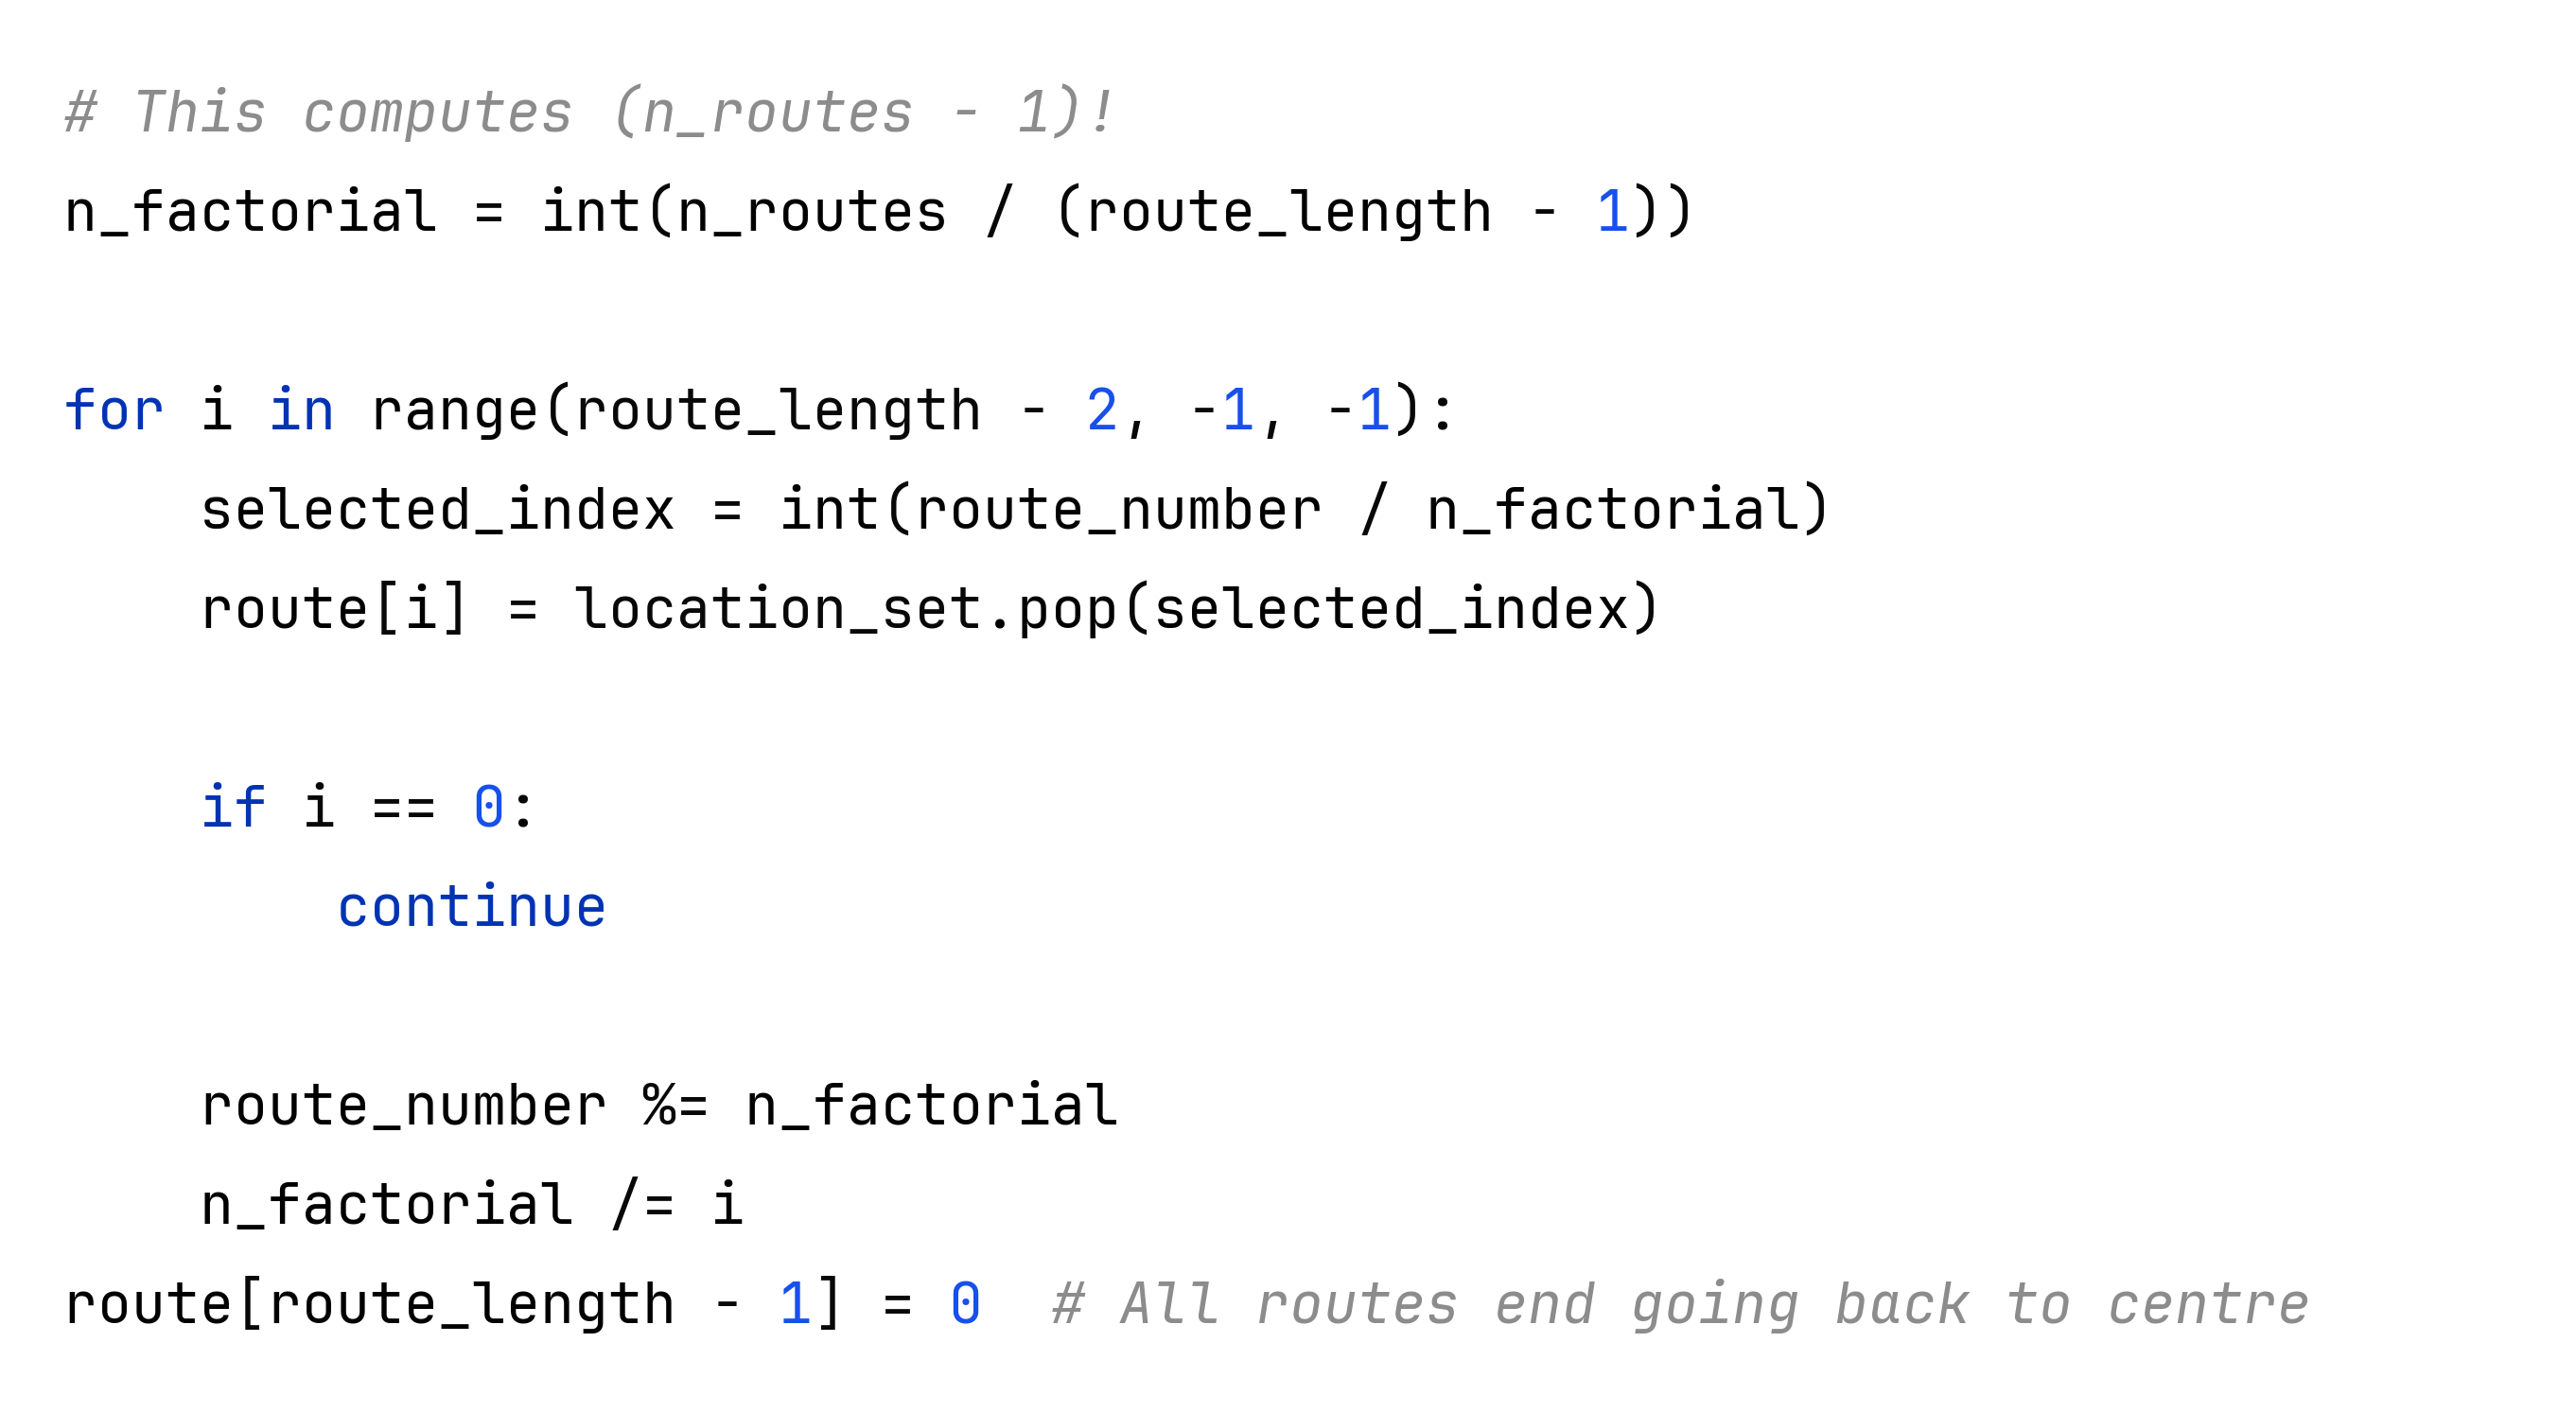
\includegraphics[width = \textwidth]{Algorithm.generate_route}
    \caption{Code from Algorithm.generate\_route in algorithms\textbackslash algorithm.py}
    \label{fig:Algorithm.generate_route}
\end{figure}

\noindent
With this method of generating routes in place, all that is required is to iterate through them all, evaluate them, and
keep track of the best found.
The implementation of this is shown in figure~\ref{fig:Routing.brute_force}.
\begin{figure}[H]
    \centering
    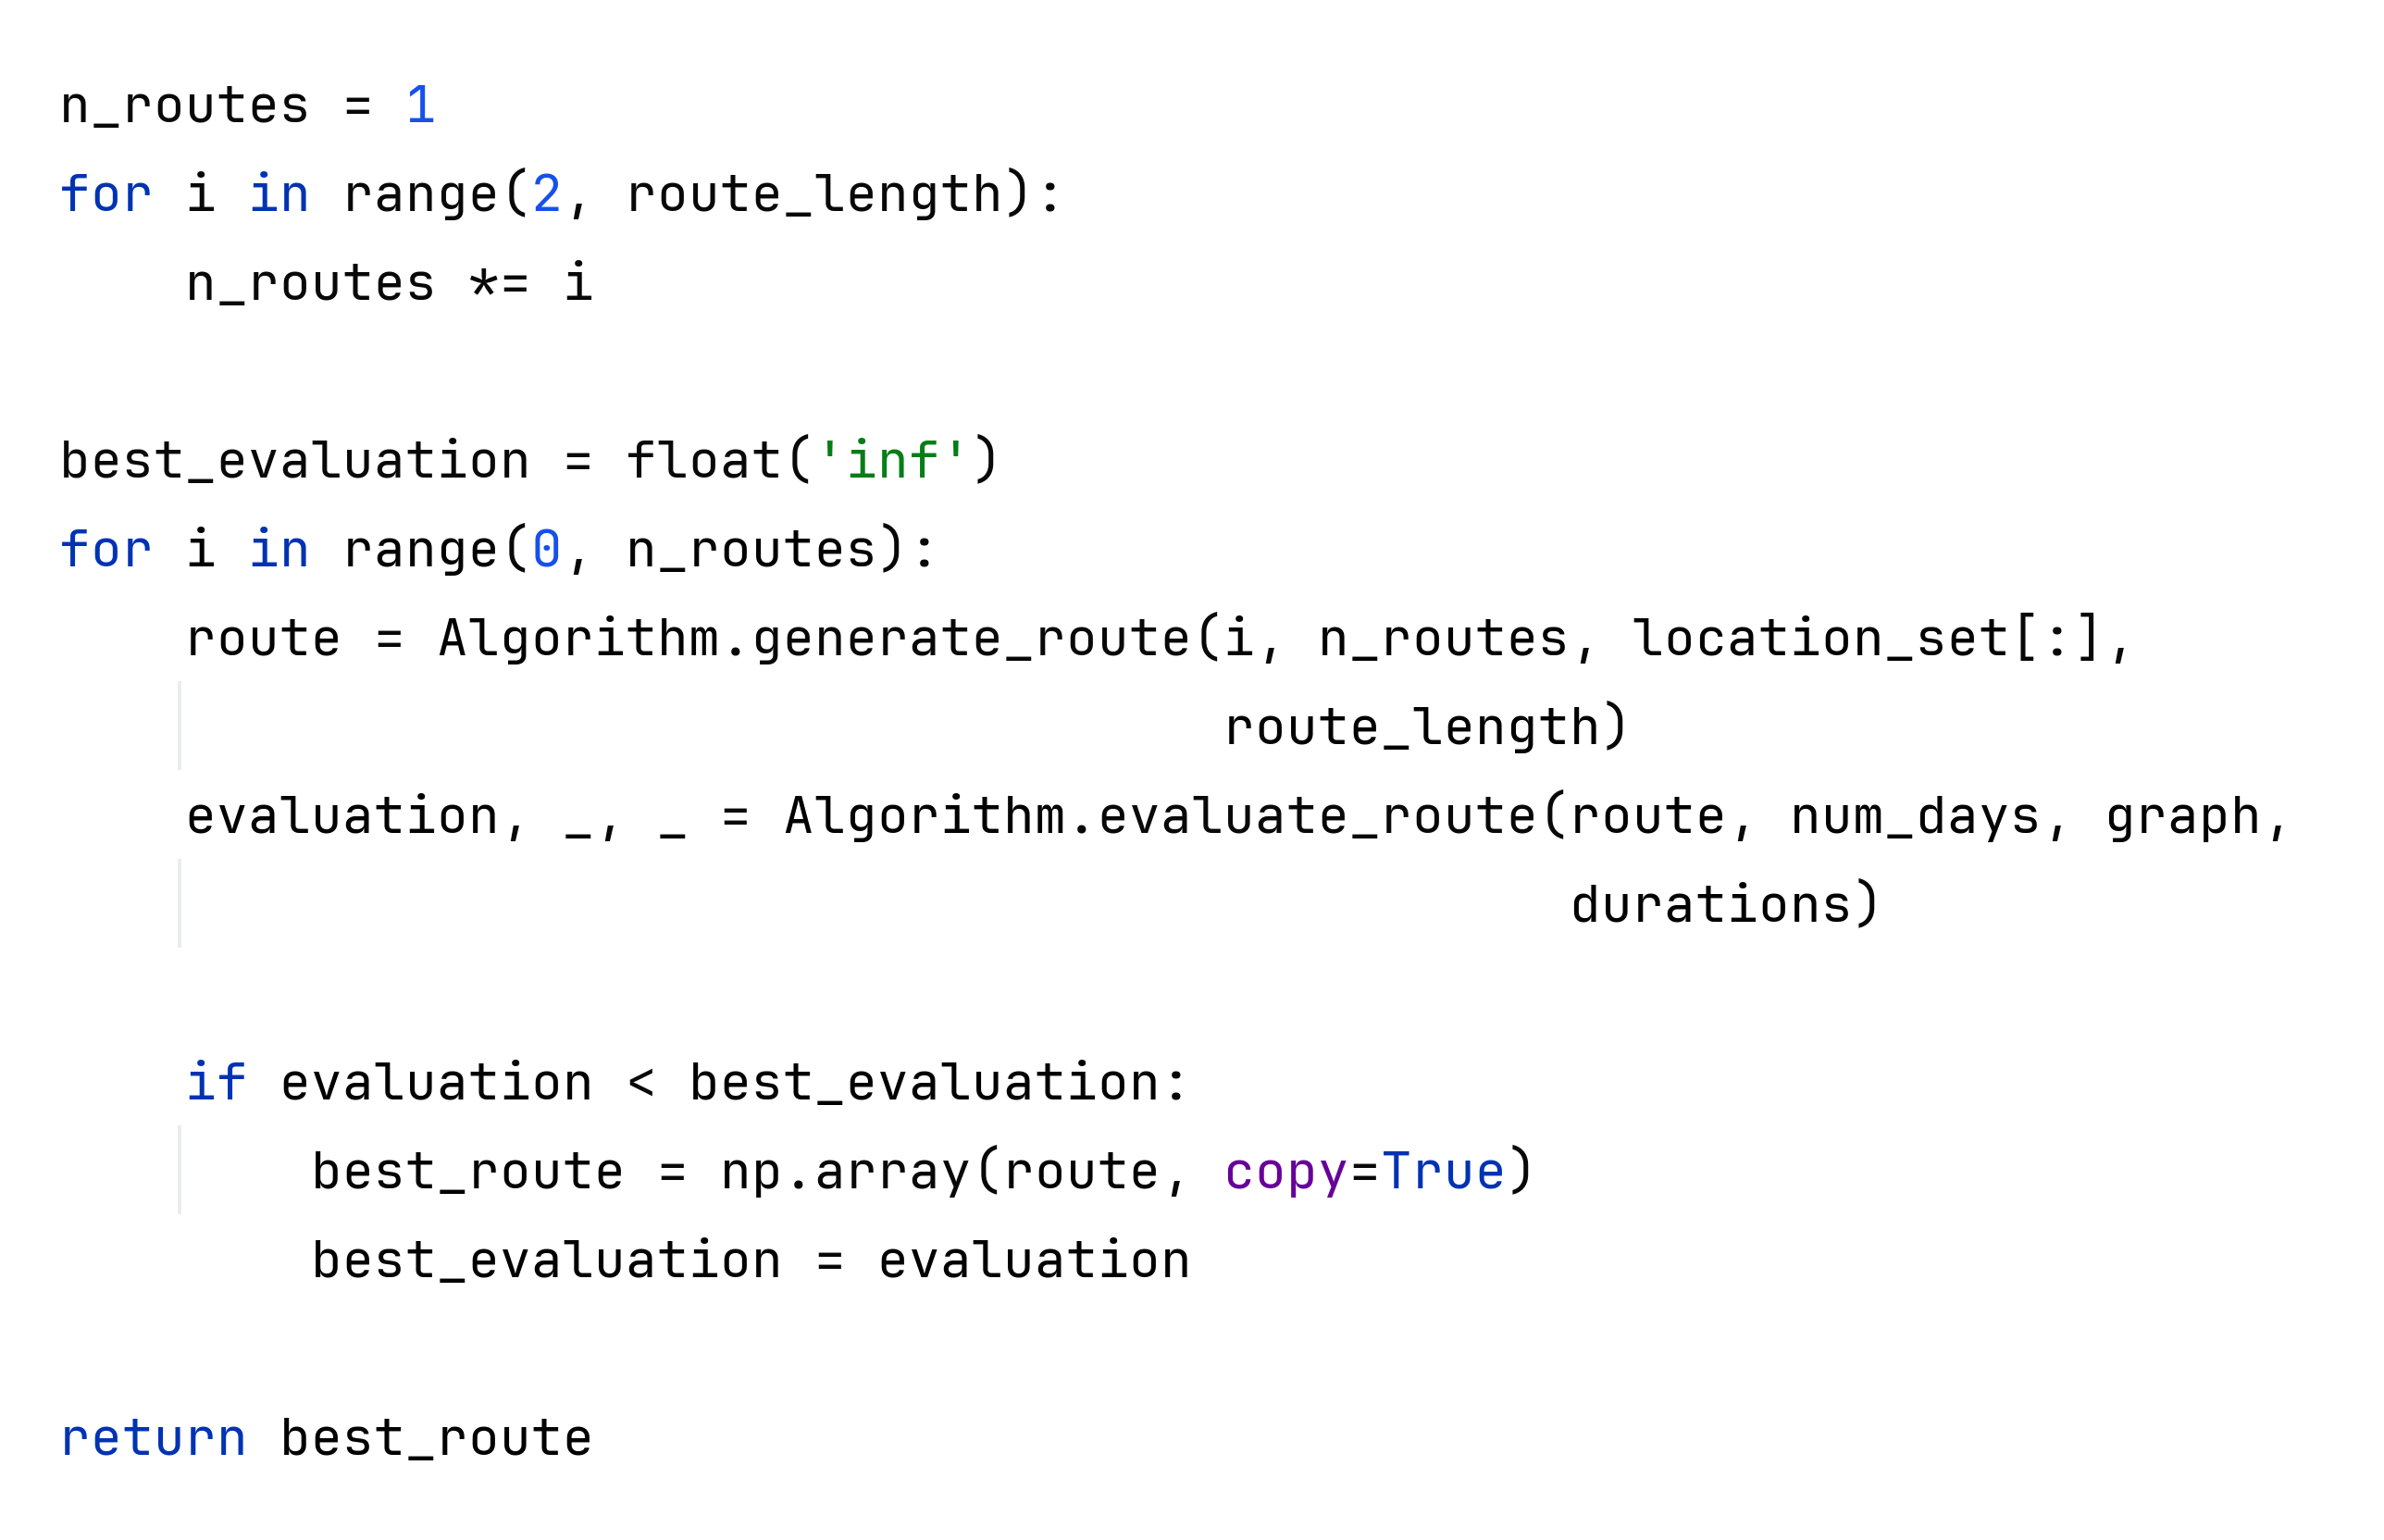
\includegraphics[width = \textwidth]{Routing.brute_force}
    \caption{Code from Routing.brute\_force in algorithms\textbackslash routing.py}
    \label{fig:Routing.brute_force}
\end{figure}

\noindent
Figure~\ref{fig:Bruteforce_Birmingham_Example} shows an example of the route find by performing Brute Force on an input
of 10 locations around Birmingham.
The location marked in green represents the starting point, and the blue marker indicates the first location
visited (showing the direction of the route).
\begin{figure}[H]
    \centering
    \includegraphics[width = \textwidth]{Bruteforce_Birmingham_Example}
    \caption{Example of a route found visiting 10 locations around Birmingham using Brute Force routing}
    \label{fig:Bruteforce_Birmingham_Example}
\end{figure}

\noindent
Being able to find a perfect route is certainly useful, but the computational cost of Brute Force becomes
impractical as the input size grows.
In calculating the 10 location route shown in figure~\ref{fig:Bruteforce_Birmingham_Example}, 362,880 possible routes
were considered, taking around 15 seconds.
If the maximum input size of 25 locations were to be used, over 620 sextillion routes would be considered \textemdash
which, assuming the same rate of routes evaluated per second, would take over 800 billion years.

While Brute Force is impractical for routing between a large number of locations, is it still useful for smaller inputs.
This may prove useful when combined with clustering algorithms, providing clusters are not too large, Brute Force
may be able to effectively find intra-cluster routes.
Furthermore, for small input sizes, Brute Force can be useful as a benchmark against which to compare other routing
algorithms.

\subsubsection{Greedy Routing}\label{subsubsec:greedy-routing}
Greedy Routing is a heuristic algorithm that builds a route iteratively, always choosing the next location according
to the shortest available path.
This is done by starting at the first location and then repeatedly selecting the next closest location until all
locations have been visited, then returning home.
At every location, the distance to every other location is checked to find the closest, giving this greedy algorithm a
time complexity of $O(n^2)$.\\

\noindent
Greedy Routing was by far the simplest algorithm to implement, and does not require much explanation.
This project's implementation will simply make a copy of the graph input, then iteratively find the closest location to
add to the route.
When a location is visited, the edges leading to it are given an infinite cost to ensure that it is not visited again.
The python implementation of Greedy Routing is shown in figure~\ref{fig:Routing.greedy_routing}.
\begin{figure}[H]
    \centering
    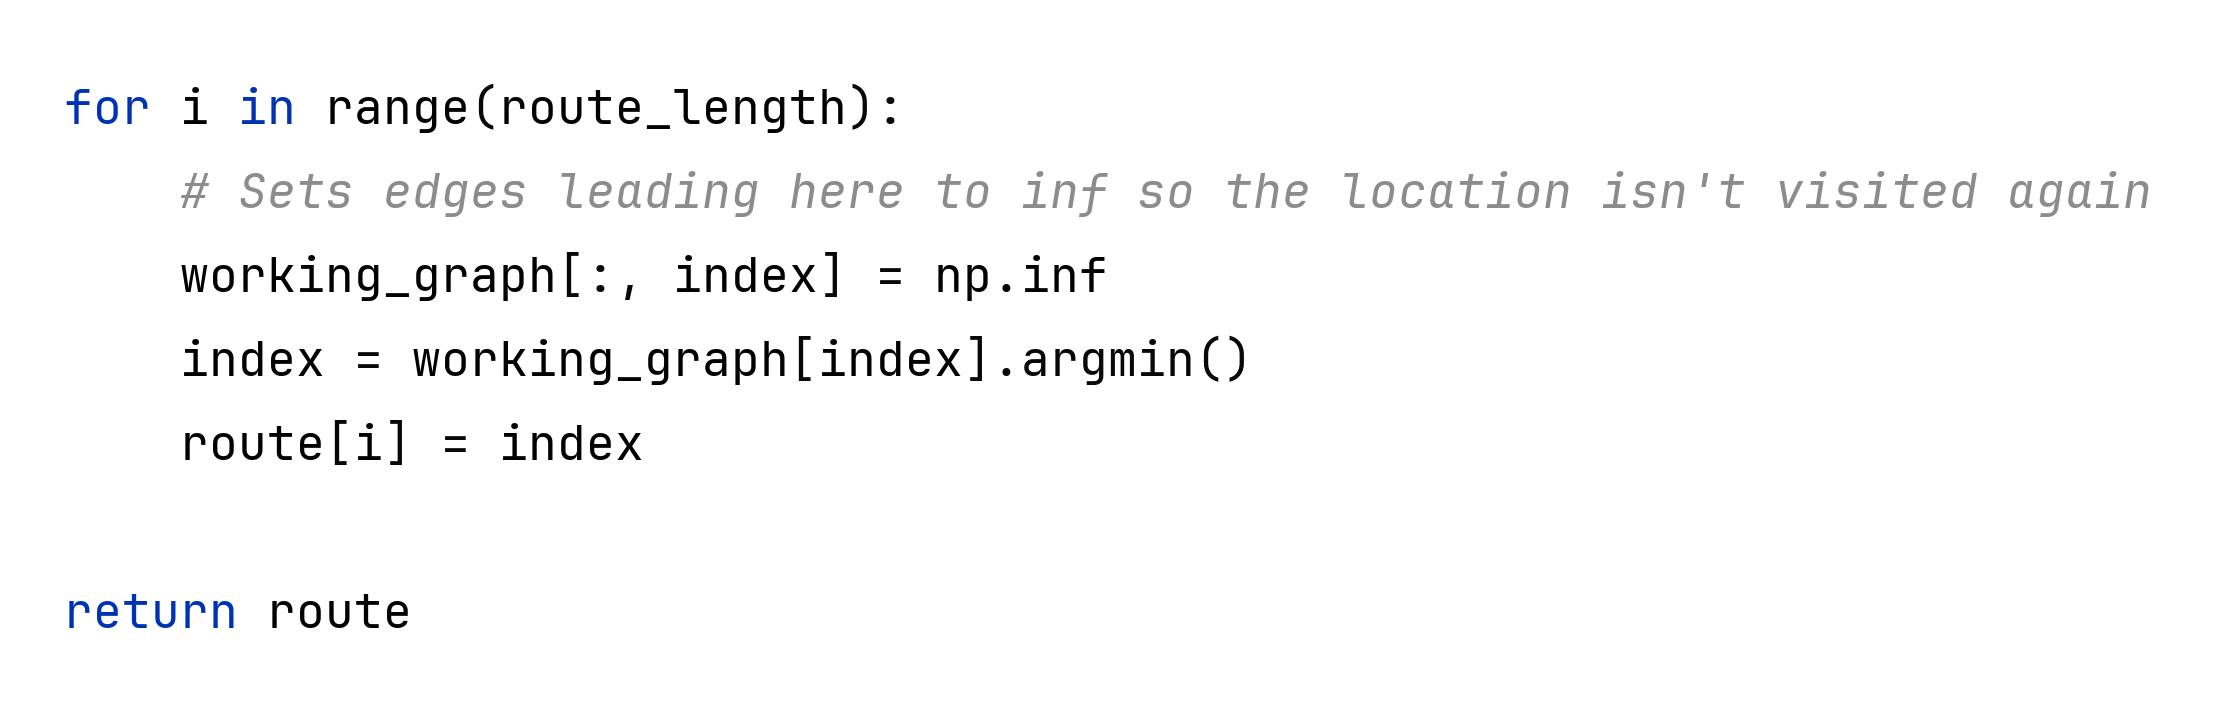
\includegraphics[width = \textwidth]{Routing.greedy_routing}
    \caption{Code from Routing.greedy\_routing in algorithms\textbackslash routing.py}
    \label{fig:Routing.greedy_routing}
\end{figure}

\noindent
Figure~\ref{fig:GreedyRouting_Birmingham_Example} shows an example of a route find by Greedy Routing, using the same
Birmingham input as that shown for Brute Force in figure~\ref{fig:Bruteforce_Birmingham_Example}.
\begin{figure}[H]
    \centering
    \includegraphics[width = \textwidth]{GreedyRouting_Birmingham_Example}
    \caption{Example of a route found visiting 10 locations around Birmingham using Greedy Routing}
    \label{fig:GreedyRouting_Birmingham_Example}
\end{figure}

\noindent
As is perhaps evident from its example, Greedy Routing isn't always a great fit, with the effectiveness of the
algorithm being highly dependent on the input.
It may just happen that for some inputs the greedy algorithm will find a good route, but as input size grows and
routes become more complex, this becomes increasingly unlikely.

Where Greedy Routing does excel, and the reason for its inclusion in this project, is in its speed.
The algorithm found a route for the 10 location Birmingham input in less than a thousandth of a second, over 500,000
times faster than Brute Force.
Some fast routing algorithms are needed in order to use alongside the genetic clustering methods which, for
evaluation, require a route to be found for every individual in a population.

\subsubsection{Greedy Insertion}\label{subsubsec:greedy-insertion}
Similar to Greedy Routing, Greedy Insertion is another heuristic algorithm that iteratively builds routes.
This time, instead of selecting the next location to add into the route, the set of unvisited locations will be iterated
through, finding the best location to insert each one into the route.
To find the best insertion point, cost of the route produced by each possible insertion point will be calculated
position, the cheapest insertion point will be chosen.
Compared to Greedy Routing, this adds an extra $O(n)$ step to each iteration, increasing the time complexity to
$O(n^3)$.\\

\noindent
While Greedy Insertion is a more complex algorithm than Greedy Routing, it is still relatively simple to implement.
All that's required is to iterate through the list of locations, evaluate the route created by inserting them at
each position, and keeping the best route each time.
The code used for Greedy Insertion can be seen in figure~\ref{fig:Routing.greedy_insertion}
\begin{figure}[H]
    \centering
    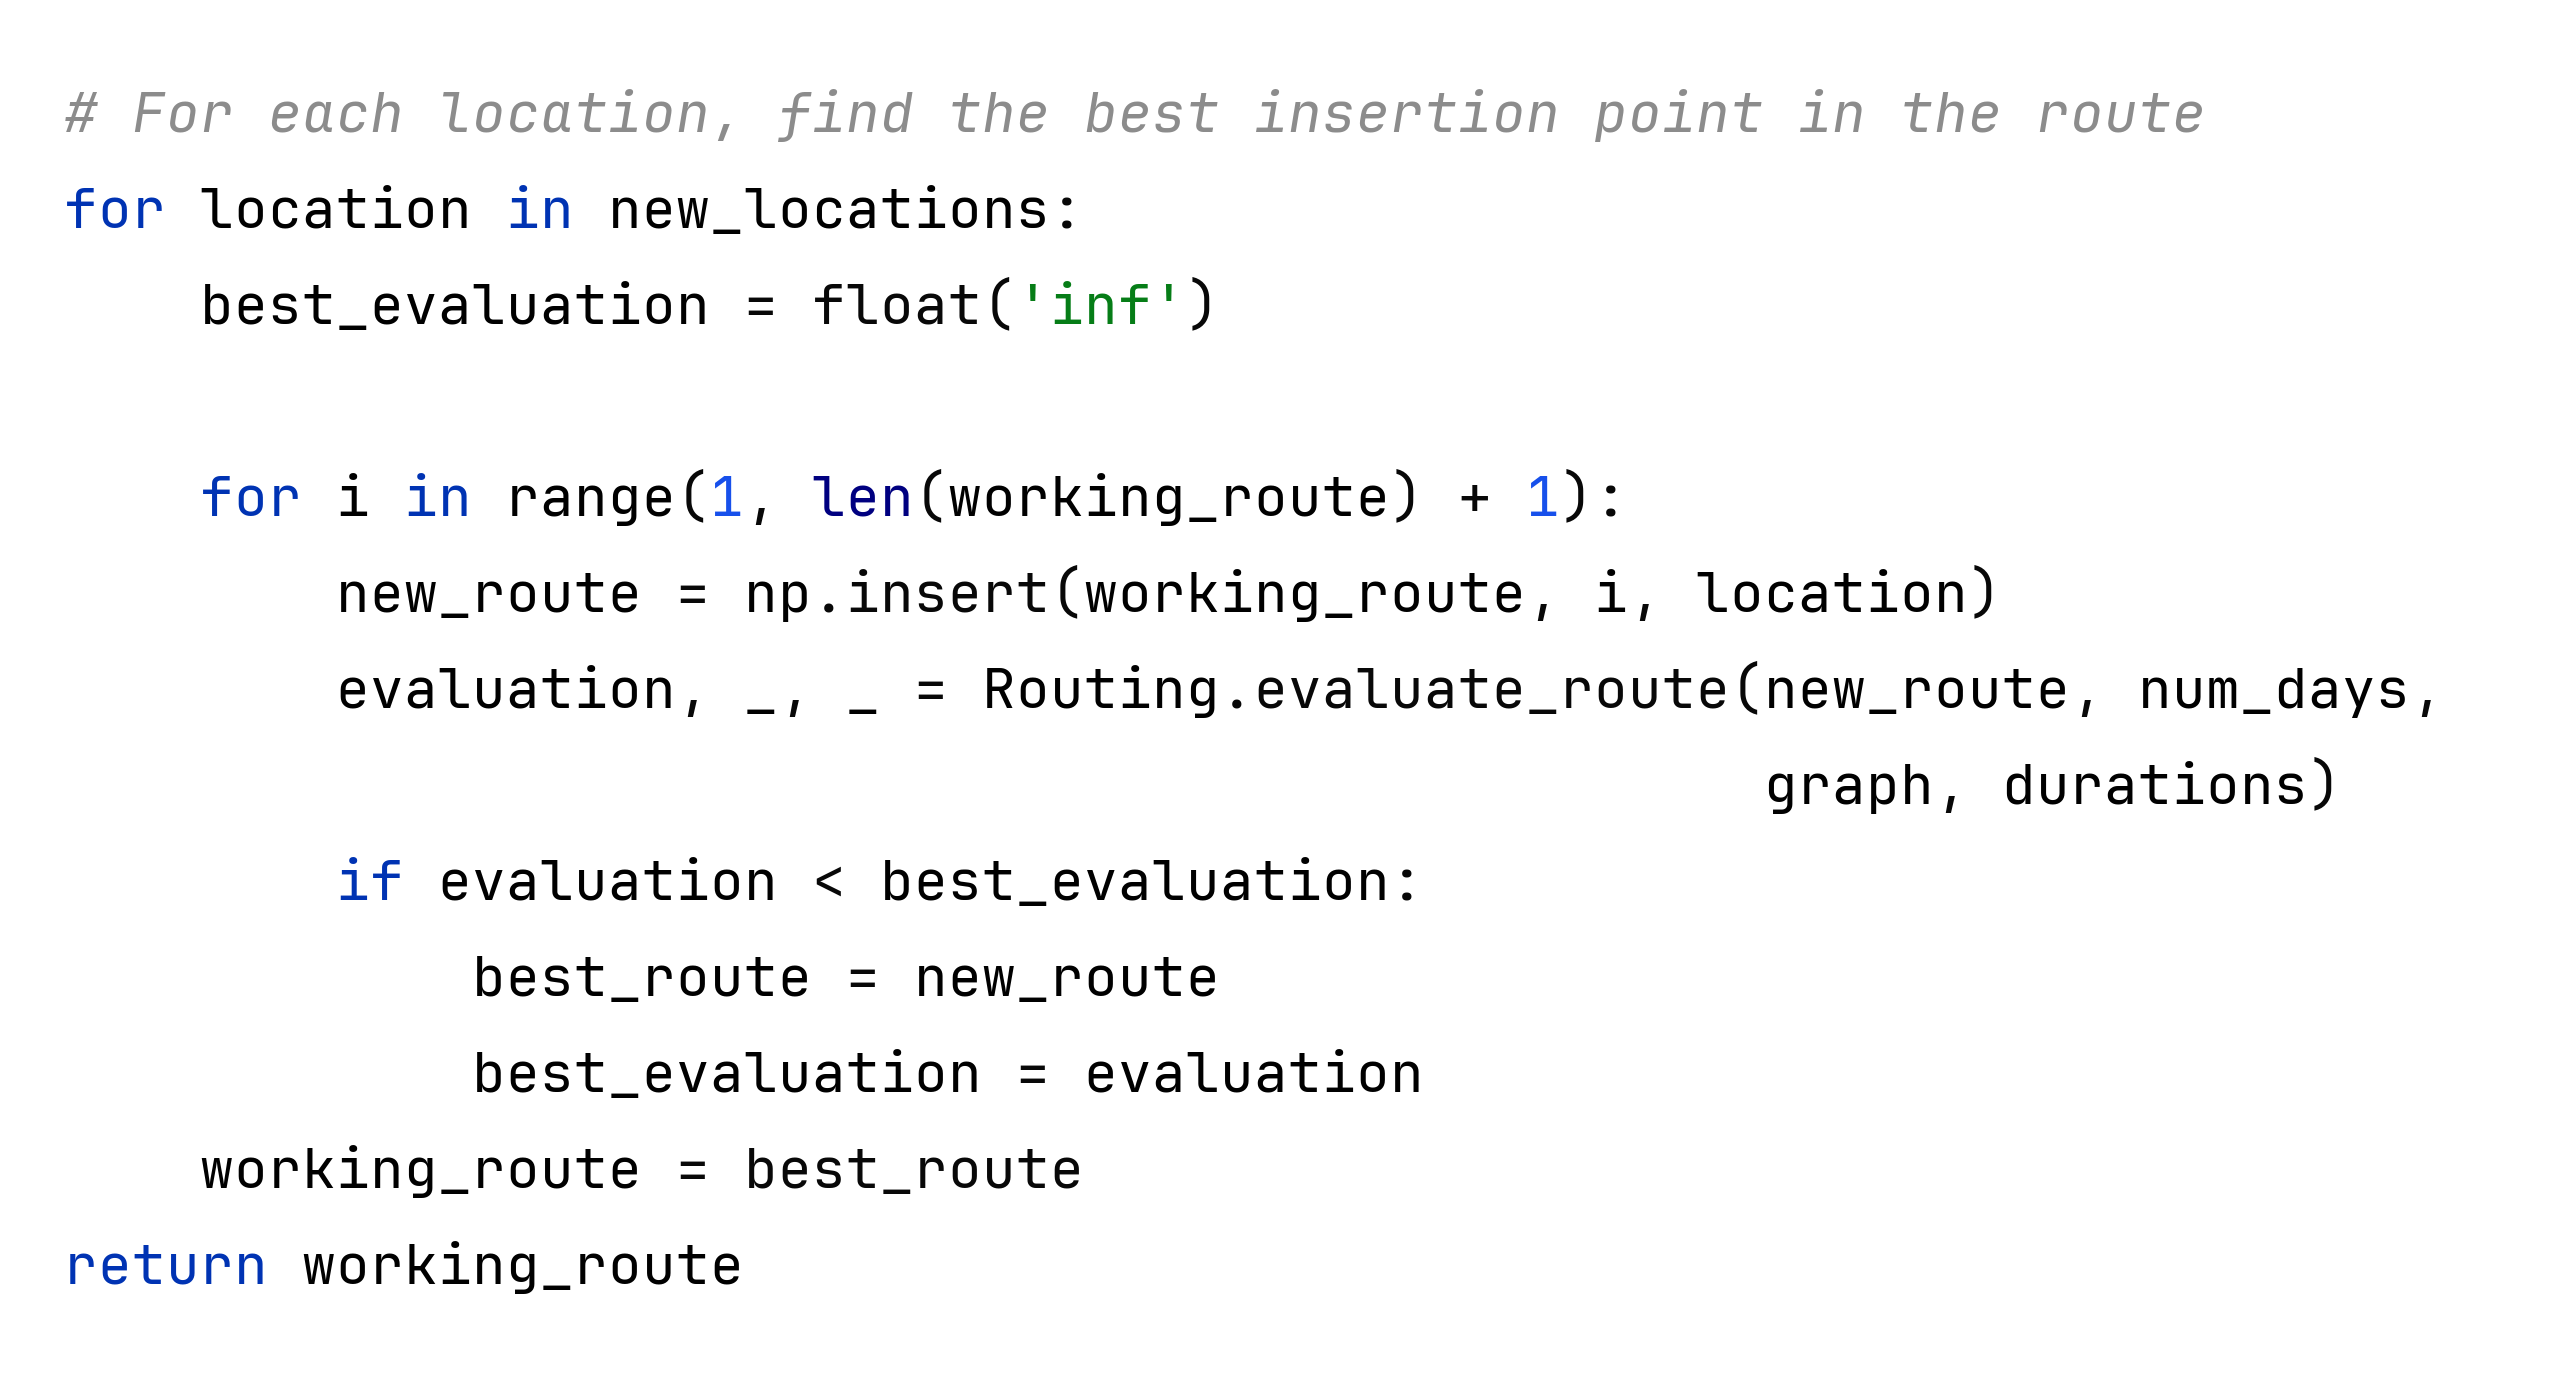
\includegraphics[width = \textwidth]{Routing.greedy_insertion}
    \caption{Code from Routing.greedy\_insertion in algorithms\textbackslash routing.py}
    \label{fig:Routing.greedy_insertion}
\end{figure}

\noindent
An example of a route found by applying Greedy Insertion to the 10 location Birmingham input is shown in figure
\ref{fig:GreedyInsertion_Birmingham_Example}.
\begin{figure}[H]
    \centering
    \includegraphics[width = \textwidth]{GreedyInsertion_Birmingham_Example}
    \caption{Example of a route found visiting 10 locations around Birmingham using Greedy Insertion}
    \label{fig:GreedyInsertion_Birmingham_Example}
\end{figure}

\noindent
For this input, Greedy Insertion was able to find the optimal solution, as indicated by it returning the same route
as Brute Force.
Finding said route took Greedy Insertion a few thousandths of a second, which while several times slower than greedy
routing, is still a huge improvement on Brute Force.
Hopefully Greedy Insertion can provide better results than Greedy Routing, without too much of a cost in terms of
time improvement.

Finding routes isn't where insertion's usefulness ends though, it can also be used to build upon existing routes,
or to split a route up into multiple days.
Perhaps a route has already been found, but there is a want to add more locations to it, Greedy Insertion can be
performed to find the best point for each location to insert into the pre-existing route.
Furthermore, if for Greedy Insertion's new locations input, a set consisting of a route's starting point $d$ number of
times is provided,  $d$ number of days can be added to form a complete trip.
This allows the creation of multi-day trips out of the routes found via the implemented routing algorithms, by taking
their routes and splitting them where Greedy Insertion believes is best.

\subsubsection{Convex Hull Routing}\label{subsubsec:convex-hull}
Given a set of points, its convex hull is the smallest border one can draw between them, such that all points are
contained inside.
For two-dimensional problems, it can be described as the shape a rubber band would take if stretched around the points.
Figure~\ref{fig:ConvexHull_Example} shows a drawing of a convex hull surrounding a set of points
\begin{figure}[H]
    \centering
    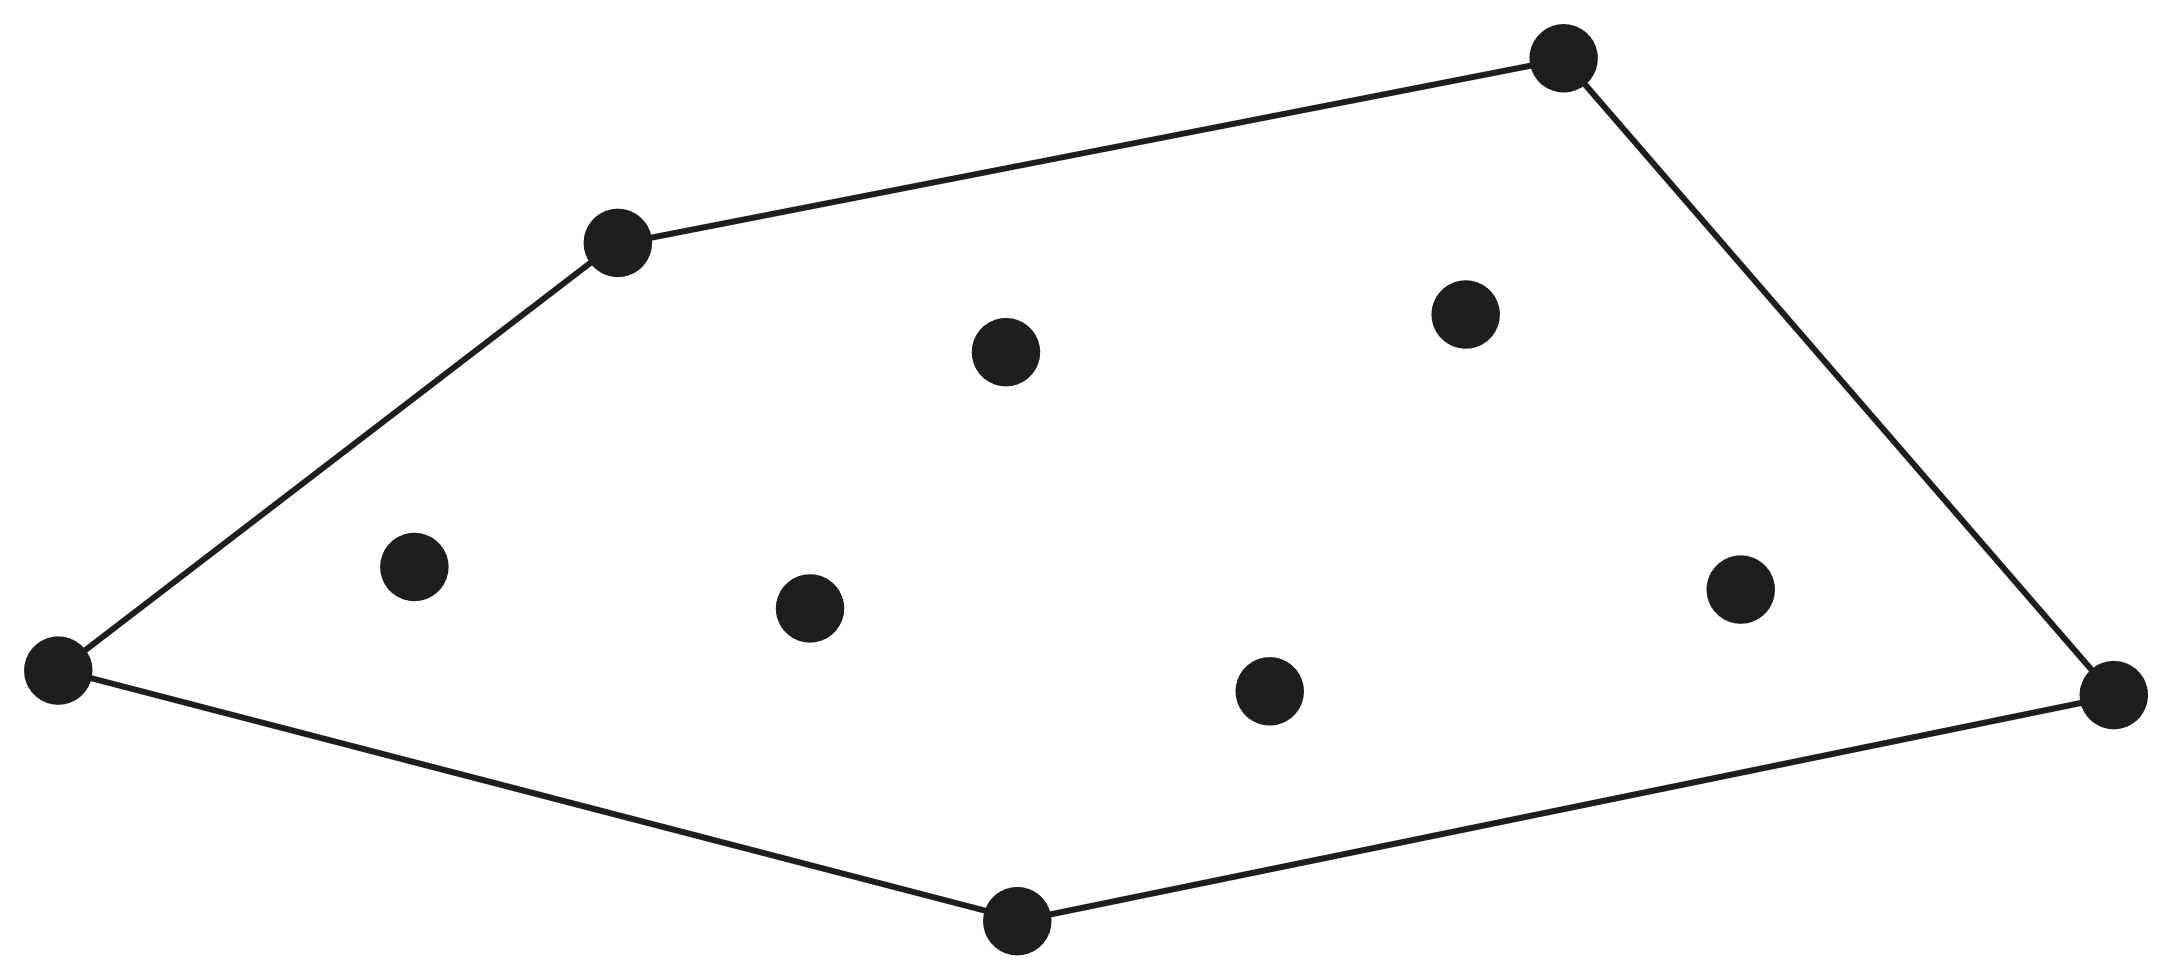
\includegraphics[width = \textwidth]{ConvexHull_Example}
    \caption{Drawing of a convex hull around a set of points}
    \label{fig:ConvexHull_Example}
\end{figure}

\noindent
If all locations happen to fall on the border of the convex hull, then the convex hull is itself an optimal route;
although, this is rather unlikely to happen.
Regardless, the convex hull does still indicate that an optimal route will visit the border cities in the order they
appear on the hull~\parencite[p. 46]{applegate2006traveling}.
With this in mind, the convex hull can be used as a starting point, before Greedy Insertion finds a complete route.
The time complexity of finding a convex hull is $O(nh)$\parencite[p. 1029]{cormen2022introduction}, where $n$ is the
number of locations, and $h$ is the number of points on the hull.
In the worst case, where all the points are on the hull, this becomes $O(n^2)$.

To find a convex hull a Gift Wrapping, or Jarvis March, algorithm will be used.
This algorithm works by finding the leftmost point in the set and then progressively finding the most counter-clockwise
point to add to the hull.
To discover the most counter-clockwise point a candidate for the next point on the hull is arbitrarily selected.
Then, for every other location not yet in the hull, the cross product is calculated: $\vec{HC} \times \vec{HI}$, where
$H$ is the most recently added hull point, $C$ is the candidate point and $I$ is the location being evaluated.
If the cross product is positive, then $I$ is more counter-clockwise than $C$, and $C$ can be replaced with $I$ as
the new candidate to be added to the hull.
When all possible values for $I$ produce a negative cross product, the candidate point is added to the hull and a new
arbitrarily selected candidate is chosen.
This process is repeated until the next hull candidate is the original starting point of the hull.

Figures~\ref{fig:Routing.gift_wrapping} and~\ref{fig:ConvexHull_Birmingham_Hull} show how this was accomplished in
python, and the hull formed around the Birmingham example, respectively.
\begin{figure}[H]
    \centering
    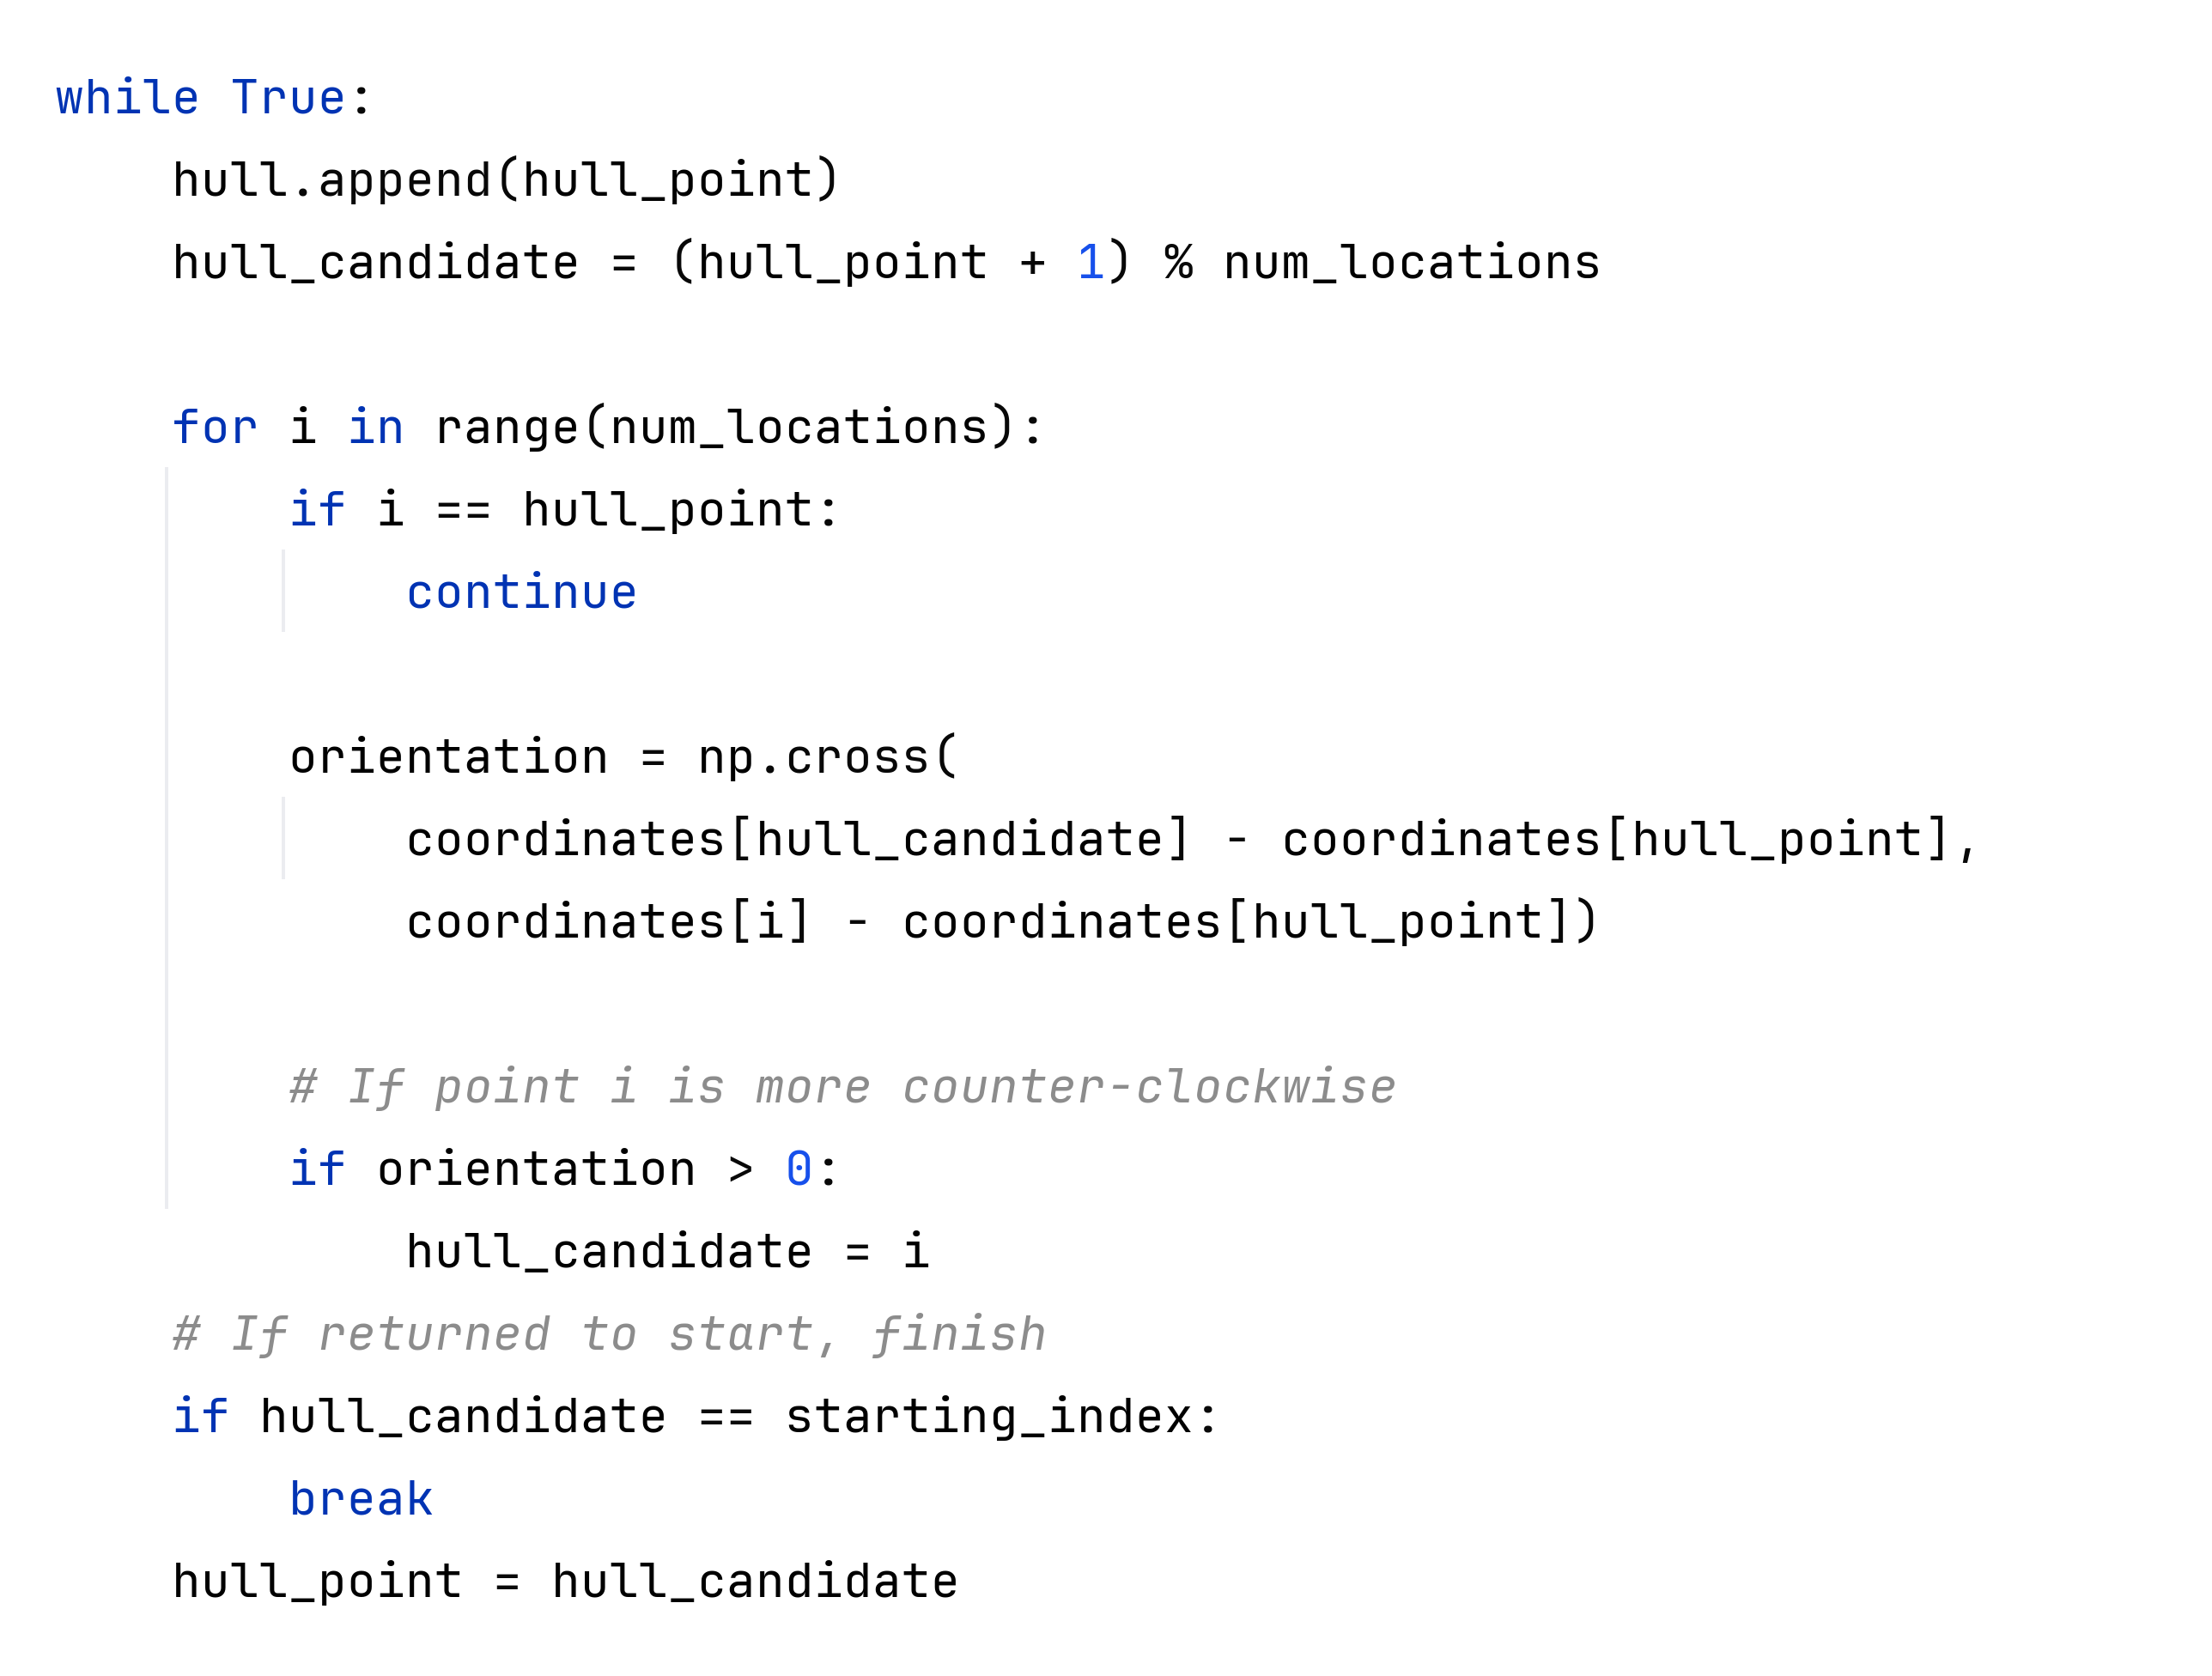
\includegraphics[width = \textwidth]{Routing.gift_wrapping}
    \caption{Code from Routing.gift\_wrapping in algorithms\textbackslash routing.py}
    \label{fig:Routing.gift_wrapping}
\end{figure}
\begin{figure}[H]
    \centering
    \includegraphics[width = \textwidth]{ConvexHull_Birmingham_Hull}
    \caption{Example of the convex hull found around 10 locations in Birmingham}
    \label{fig:ConvexHull_Birmingham_Hull}
\end{figure}

\noindent
Once the hull is found, it can be used as a starting point for Greedy Insertion.
This hull will be used as a starting point for a route, and all the interior points as locations for insertion.
Figure~\ref{fig:ConvexHull_Birmingham_Route} shows the route found by applying Greedy Insertion to the hull found
around the Birmingham example.
\begin{figure}[H]
    \centering
    \includegraphics[width = \textwidth]{ConvexHull_Birmingham_Route}
    \caption{Example of a route found using Greedy Insertion and the convex hull of 10 locations in Birmingham}
    \label{fig:ConvexHull_Birmingham_Route}
\end{figure}

\noindent
Convex Hull Routing was included in this project to investigate how well it would work as a starting point for greedy
insertion.
It will be interesting to see whether starting from a convex hull could improve the results and/or the speed of
Greedy Insertion, as opposed to running Greedy Insertion on the whole set of locations.

\subsubsection{Genetic Routing}\label{subsubsec:genetic-routing}
As well as clustering, genetic algorithms can also be used for routing.
We will evolve a population of potential routes similarly to before, this time with each genome representing a
potential route, and with new crossover and mutation techniques to account for this.
Without the need to use another routing algorithm in order to evaluate its population, genetic routing has a
slightly faster time complexity of $O(g p n)$, with $g$ being the number of generations, $p$ being the population
size and $n$ being number of locations in the route.\\

\noindent
By finding a route directly, selection is simpler, no longer requiring the use a routing algorithm with each genome
to find a route capable of evaluation.
This time, a genome will represent a permutation of the locations to be visited, with the order of the locations in the
genome representing the order in which they will be visited, similar to the Brute Force algorithm.
We will be selecting the best individuals in a population by evaluating the route formed in their genome.
Via crossover and mutation, the order in which locations are visited will be shuffled to try and find a better
route.
The crossover algorithm will be a simple single-point crossover, a random point in the genome will be chosen and all
locations up to that point will be taken from one parent.
Then, all the remaining locations will be added in the order they appear in the second parent's genome.
A simple example of single-point crossover is shown in figure~\ref{fig:Point_Crossover_Example}, using two
hypothetical genomes with 6 locations.
The python implementation of this crossover method is shown in figure~\ref{fig:GeneticRouting._crossover}.
\begin{figure}[H]
    \centering
    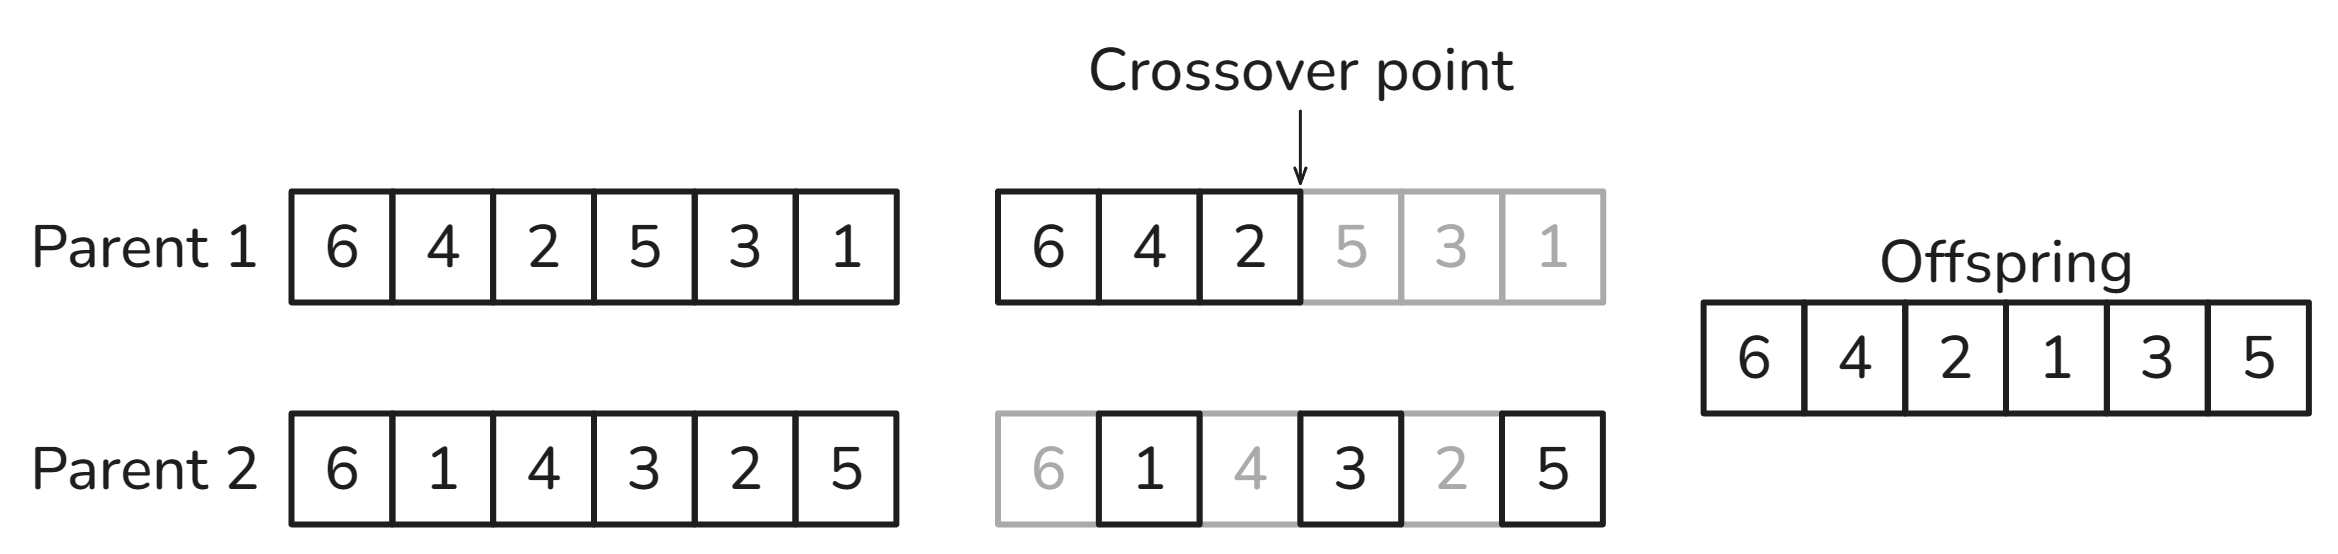
\includegraphics[width = \textwidth]{Point_Crossover_Example}
    \caption{Example of using single point crossover to create offspring from two parents.}
    \label{fig:Point_Crossover_Example}
\end{figure}
\begin{figure}[H]
    \centering
    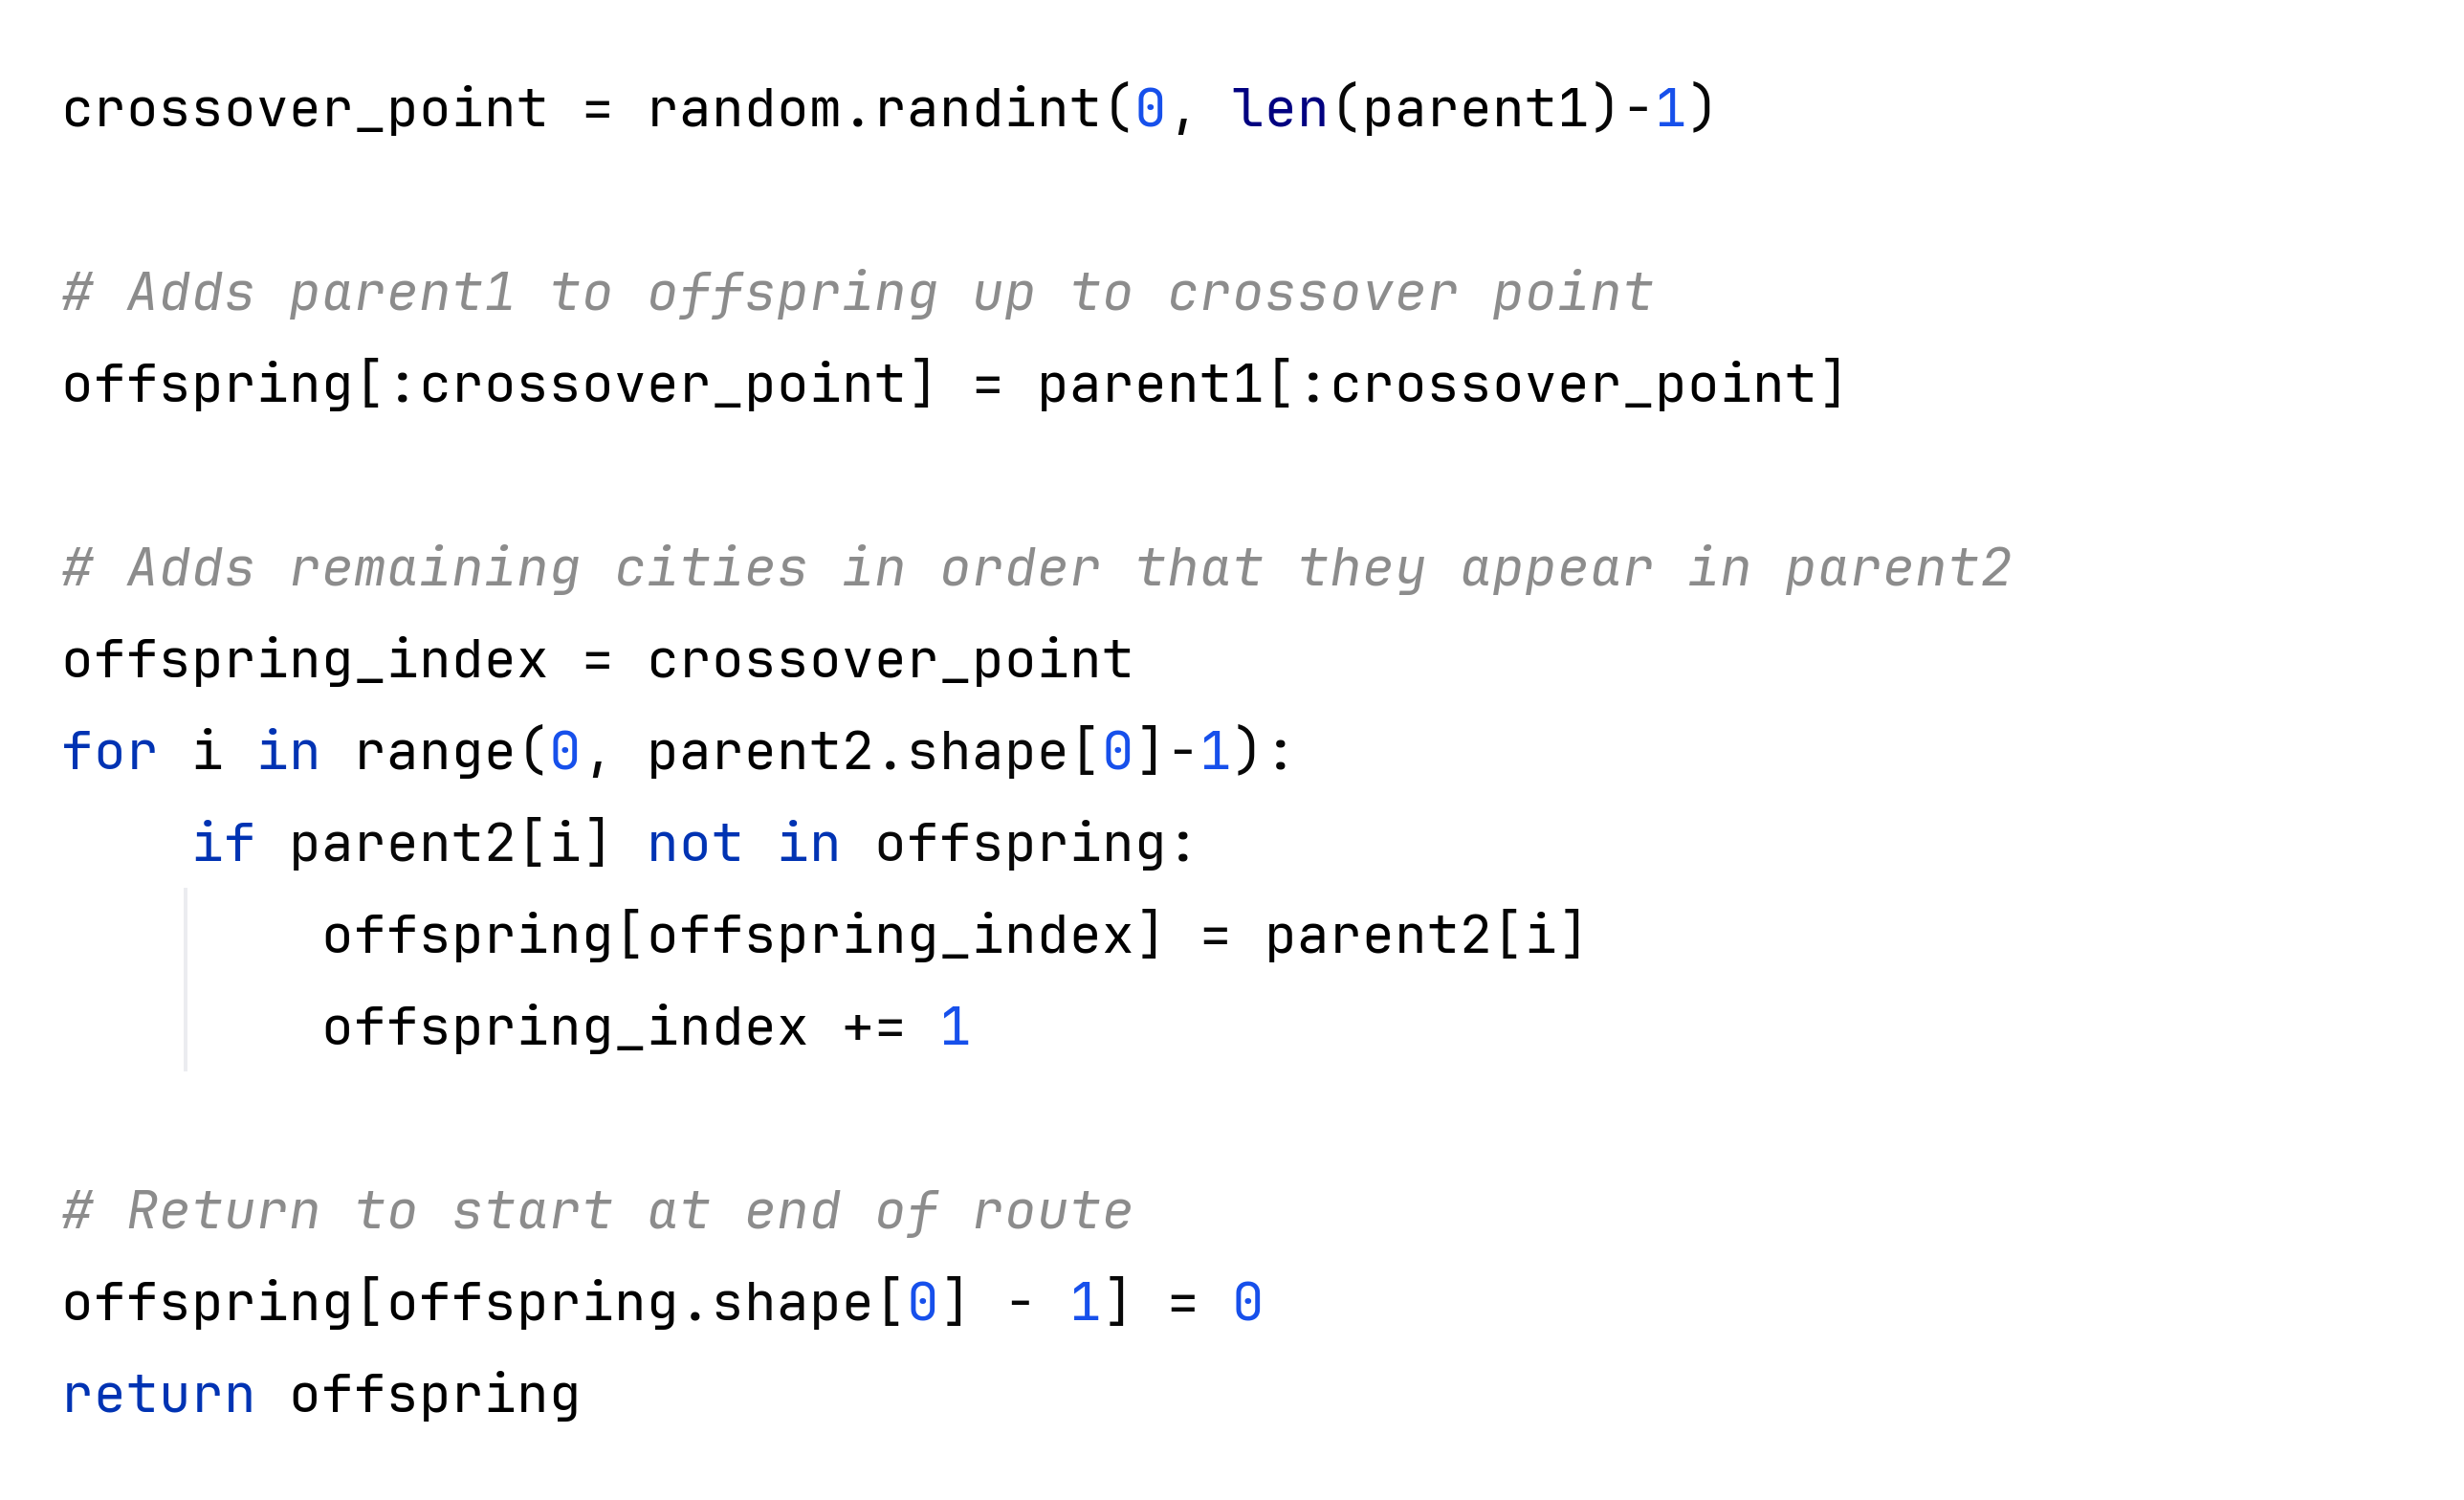
\includegraphics[width = \textwidth]{GeneticRouting._crossover}
    \caption{Code from GeneticRouting.\_crossover in algorithms\textbackslash routing.py}
    \label{fig:GeneticRouting._crossover}
\end{figure}

\noindent
For mutation, a number of individuals will be randomly chosen to mutate inline with the algorithms mutation
probability.
Chosen individuals will have two locations in their route randomly chosen and swapped.
This implementation is shown in figure~\ref{fig:GeneticRouting.mutation}, the final location isn't considered for
swapping, as all routes end at the starting point.
\begin{figure}[H]
    \centering
    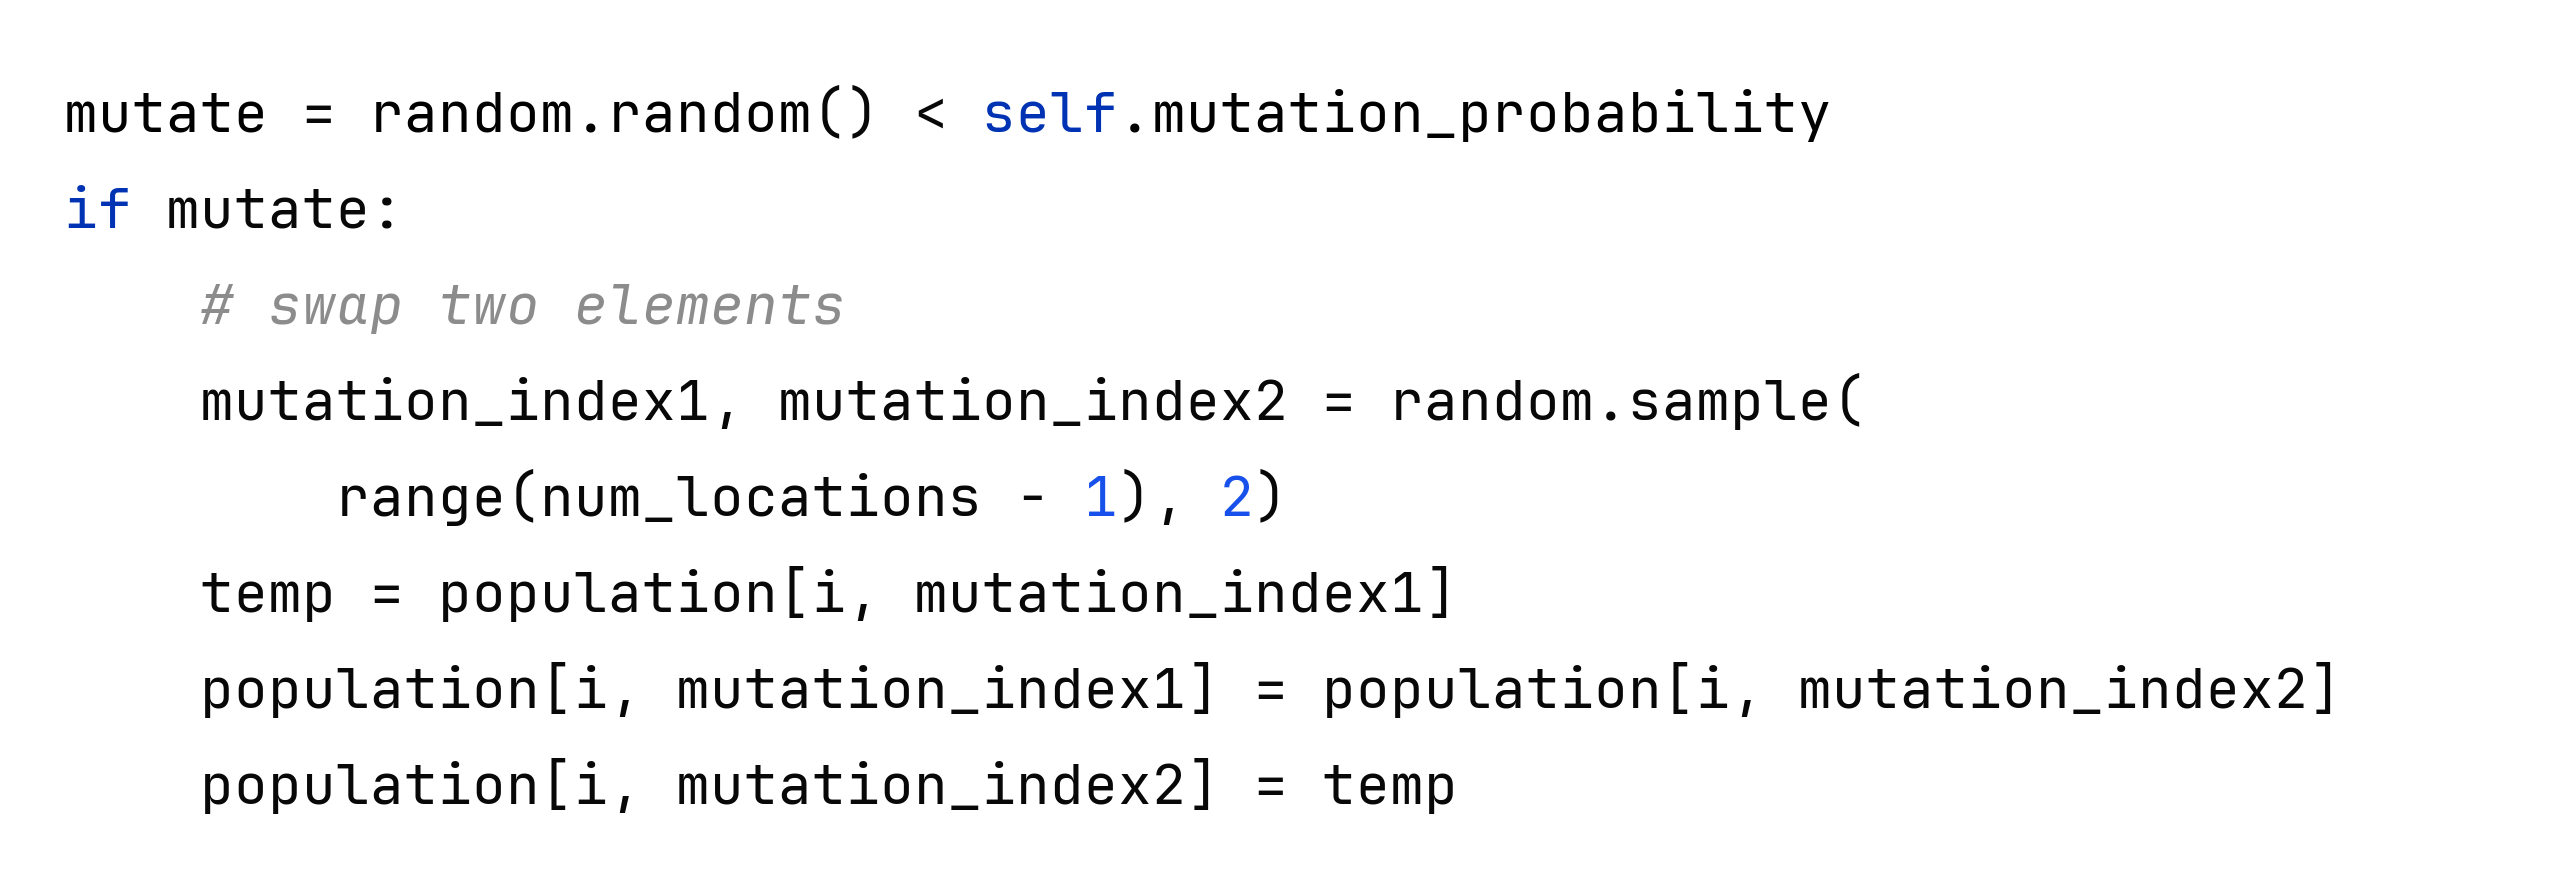
\includegraphics[width = \textwidth]{GeneticRouting.mutation}
    \caption{Code from GeneticRouting.find\_route in algorithms\textbackslash routing.py}
    \label{fig:GeneticRouting.mutation}
\end{figure}

\noindent
By repeatedly performing selection, crossover and mutation the population will hopefully converge on a better route.
Figure~\ref{fig:GeneticRouting_Birmingham_Generation1} shows an example of genetic routing performed on the 10
location Birmingham input.
For this example, 30 generations were evolved with a population size of 12, a crossover rate of 0.9 and a mutation
rate of 0.4.
A line graph of the best evaluation found for each generation is shown in figure~\ref{fig:GeneticRouting_Birmingham_Evaluations}.
\begin{figure}[H]
    \ContinuedFloat*
    \centering
    \includegraphics[width = \textwidth]{GeneticRouting_Birmingham_Generation1}
    \caption{Genetic Routing example, best route found in Generation 1.}
    \label{fig:GeneticRouting_Birmingham_Generation1}
\end{figure}
\begin{figure}[H]
    \ContinuedFloat
    \centering
    \includegraphics[width = \textwidth]{GeneticRouting_Birmingham_Generation5}
    \caption{Genetic Routing example, best route found in Generation 5.}
    \label{fig:GeneticRouting_Birmingham_Generation5}
\end{figure}
\begin{figure}[H]
    \ContinuedFloat
    \centering
    \includegraphics[width = \textwidth]{GeneticRouting_Birmingham_Generation10}
    \caption{Genetic routing example, best route found in Generation 10.}
    \label{fig:GeneticRouting_Birmingham_Generation10}
\end{figure}
\begin{figure}[H]
    \ContinuedFloat
    \centering
    \includegraphics[width = \textwidth]{GeneticRouting_Birmingham_Generation30}
    \caption{Genetic Routing example, best route found in Generation 30, evolution is now complete.}
    \label{fig:GeneticRouting_Birmingham_Generation30}
\end{figure}
\begin{figure}[H]
    \centering
    \includegraphics[width = \textwidth]{GeneticRouting_Birmingham_Evaluations}
    \caption{Line graph showing the best evaluation for each generation of routing evolution process.}
    \label{fig:GeneticRouting_Birmingham_Evaluations}
\end{figure}

\noindent
Having implemented a number of heuristic approaches to finding routes, as well as the exact Brute Force method,
genetic routing was included to see how a more meta-heuristic algorithm might perform.
Likely to take longer than the other approximate routing methods, we'll have to see if genetic routing can make up
for this time with the quality of its results.
Hopefully genetic routing can strike a balance between fast approximate methods and the slow, exact Brute Force method.

Additionally, the suitability of genetic algorithms for routing purposes can be evaluated and compared with the
implemented genetic clustering approaches.
It is possible that genetic algorithms are only practically applicable to a certain approaches, being unable to form
good solutions for others.

\subsection{Trip Generation}\label{subsec:trip-generation}
We have now discussed how routing can be combined with both clustering and insertion to form complete trips, but
there is still one more approach that will be considered in this project.
By modifying a few existing routing algorithms namely Brute Force, Greedy Insertion and genetic routing, they can be
used to generate full trips in one go.
If the locations input for these algorithms is expanded, to include the starting point of the trip $d$ times, the same
algorithms can be used to find a multi-day trip.
For Brute Force and genetic routing, this means the permutations being considered is expanded to include returning to
the starting point $d$ times.
For Greedy Insertion, this means that all locations on the trip will first be inserted into the route, before inserting
each return to the start.

Trip generation methods directly produce whole trips instead of needing some compound approach of clustering
and routing or routing and insertion.
These algorithms were extended to include trip generation to investigate how the approach compared, by
forming a route in one stage these algorithms may more effectively minimise cost than by combining two algorithms which
take different approaches to finding an optimal solution.

    \pagebreak

    \section{Implementation}\label{sec:implementation}

    \subsection{Constraints}\label{subsec:implementation-constraints}

    \pagebreak

    \section{Evaluation and Comparison}\label{sec:evaluation-and-comparison}
    \todo{Write paragraph about experiment process. Comparison based on computation time and route evaluation.
    Describe how route is evaluated. Describe data being tested on.}
    \todo{Present comparison of different combinations of algorithms on different inputs.}
    \todo{Reflect about the questionns you are trying to answer with your evaluation. You can have onne subsection for each question that you are trying to answer. It's also important to justify your choices when it comes to the methodology used for evaluation.}

    \pagebreak

    \section{Conclusion and Future Work}\label{sec:conclusion-and-future-work}
    \todo{Write conclusion, discuss results, comparison of algorithms, etc.}
    \subsection{Project Reflection}
    \todo{Reflect on the project, what went well, what didn't go well, what I would do differently. This should lead into future work.}
    \subsection{Future work}\label{subsec:future-work}
    \todo{Discuss further work, what I will be doing to improve the project}

    \pagebreak

    \section{Bibliography}\label{sec:bibliography}
    \printbibliography
\end{document}